\chapter{Evaluation}
\label{chapter:evaluation}
\epiquote{I counted everything. I counted the steps to the road, the steps up to church, the number of dishes and silverware I washed... anything that could be counted, I did.}{Katherine Johnson, 2005}

In this chapter we present the evaluation of \cottontail{} \cite{Gasser:2020Cottontail}, which implements the previously described concepts and has become an integral part of the \vitrivr{} \cite{Rossetto:2016Vitrivr,Gasser:2019Towards,Gasser:2019Multimodal} stack. This quantitative evaluation is structured around three experiments that highlight three different aspects:

\begin{description}
    \item[Multimedia Analytics Workloads] This experiment tries to simulate multimedia analytics workloads on million-scale datasets, for which \cottontail{} was primarily designed. We demonstrate \cottontail{}'s versatility and discuss and compare different execution strategies. We use the Vimeo Creative Commons Collection 1 \& 2 (V3C) \cite{Berns:2019V3C1,Rossetto:2021Insights}, which currently serves as the reference dataset for both \acrshort{vbs} \cite{Schoeffmann:2019Video} and TRECVID AVS \cite{Chen:2021What}. The dataset consists of  \SI{17235}{} videos, which amounts to \SI{2300}{\hour} of content. We use a series of features derived by \vitrivr{}'s feature extraction engine Cineast.
    \item[Large-Scale Similarity Search] In this benchmark, we test \cottontail{}'s ability to scale out to very large datasets as employed in challenges such as the (Big-) ANN-Benchmark \cite{Aumueller:2017ANN,Simhadri:2022Results}. While not the primary focus of \cottontail{}'s design, this is still an interesting task to obtain a baseline for future efforts. We use this opportunity to compare \cottontail{} to Milvus (see \Cref{section:milvus}) in a series of large-scale \acrshort{nns} queries. All queries are run against shards of the Yandex Deep1B dataset \cite{Babenko:2016Efficient}, which is a collection of descriptors derived from a GoogLeNet \cite{Szegedy:2015Going} neural network.
    \item[High-Dimensional Index Maintenance] In this experiment we examine how \cottontail{} copes with incremental changes to the dataset that take place concurrently to query activities. We demonstrate its ability to implement such changes in the presence of indexes. Finally, we test the proposed mechanisms for concurrent index rebuilding.
\end{description}

\section{Evaluation Setup}

The entire evaluation is centred around database queries that are sent to the system under testing. We generate measurements from these queries and the results they return. Typically, we average the obtained values over $10$ repetitions to compensate for anomalies and we execute a single warm-up query to give the systems the ability to initialise necessary caches (exceptions are mentioned explicitly). 

Rather than working with randomly generated data, we decided to use existing data corpora that reflect the structure of features as generated by different models. For that, we use the Vimeo Creative Commons Collection (V3C) \cite{Berns:2019V3C1,Rossetto:2021Insights} and the Yandex Deep1B dataset \cite{Babenko:2016Efficient}. For V3C, we rely on features generated by our own extraction engine Cineast \cite{Rossetto:2016Vitrivr} and from the Deep1B dataset we have prepared different shards that contain the first 5 million, 10 million, 100 million, and all 1 billion pre-generated feature vectors. All data is imported as a dedicated entity (\cottontail{}) or collection (Milvus) respectively, prior to executing the actual workloads. A list of all datasets and the resulting entities is provided in \Cref{table:datasets} and we will refer to the collections and entities by their name throughout this chapter.
Necessary index structures are prepared beforehand if not stated otherwise. Every entity exhibits the columns \texttt{id} and \texttt{feature}. The \texttt{id} column serves as a primary key and is either a \texttt{string} (all V3C-based datasets) or a \texttt{long} value (all Deep1B-based datasets). The Deep1B shards also exhibit an additional \texttt{category} column, which holds a randomly assigned \texttt{int} value that is used for Boolean filtering. The state of all collections is listed in \Cref{chapter:appendix_supplementals}.

\begin{table}
    \begin{tabular}{ | l | c | c | c | p{5cm} |}
        \hline
        \textbf{Entity} & \textbf{Source} & \textbf{d} & \textbf{N} & \textbf{Description} \\
        \hline
        \hline
        cineast\_segment & V3C1\&2  & - & 2512715 & Segment metadata for V3C2. Does not contain any vectors. \\ 
        \hline
        averagecolor & V3C1\&2  & 3 & 2512715 & Average colours derived from video segments. \\ 
        \hline
        visualtextcoembedding & V3C1\&2 & 25 & 2506273 & Video to text co-embedding derived from vide segments. See \cite{Spiess:2021Competitive}. \\
        \hline
        hogmf25k512  & V3C1\&2  & 512 & 2500943 & HOG \cite{Bay:2006surf} descriptors derived from video segments. \\
        \hline
        inceptionresnetv2 & V3C1\&2  & 1536 & 2508358 & Vector derived from the last fully connected layer of a pre-trained InceptionResNetV2 applied on video segments.\\
        \hline
        conceptmasksade20k & V3C1\&2 & 2048 & 2469844 & Image embedding for query by semantic sketch. See \cite{Rossetto:2019Query}. \\
        \hline
        yandex\_deep5M  & Deep1B  & 96 & $5000000$ & See \cite{Babenko:2016Efficient} for more details. \\
        \hline
        yandex\_deep10M  & Deep1B & 96 & $10000000$ & See \cite{Babenko:2016Efficient} for more details. \\
        \hline
        yandex\_deep100M  & Deep1B & 96 & $100000000$ & See \cite{Babenko:2016Efficient} for more details. \\
        \hline
        yandex\_deep1B  & Deep1B & 96 & $1000000000$ & See \cite{Babenko:2016Efficient} for more details. \\
        \hline
        \hline
    \end{tabular}
    \caption{The data collections used for this evaluation. }
    \label{table:datasets}
\end{table}

Both \cottontail{} and Milvus are deployed on the same physical server (but they do not run at the same time). This server exhibits two \acrshort{numa} nodes with an Intel Xeon CPU E5-2630 v4 (20 cores@\SI{2.2}{\giga\hertz}) and \SI{192}{\giga\byte} \acrshort{ram} each. Therefore, the machine provides 40 compute cores and a total of \SI{384}{\giga\byte} of \acrshort{ram}. The \acrshort{cpu} supports the AVX2 instruction set extension, which allows for vectorised execution. The data directories from which Milvus and \cottontail{} access their data resides on three \SI{500}{\giga\byte} \acrshort{ssd}s that have been combined into a single, logical disk using \acrshort{raid}0 (striping). The server runs Ubuntu 20.04 and the OpenJDK Java version 17.0.3. All benchmarks are orchestrated by and sent from a separate node on the same network to minimise the impact on query execution. The evaluation scripts we used are available online\footnote{See https://github.com/ppanopticon/cottontaildb-evaluation/; accessed July 2022.}.

The binary version of \cottontail{} is started with a minimum and maximum heap size of \SI{64}{\giga\byte} and \SI{256}{\giga\byte} respectively. We have setup \cottontail{}'s cost model so that it parallelises workloads aggressively, whereas, by default, it tries to balance resource use per query and expected speed-up gained. The set of configuration parameters including explanation can also be found in \Cref{chapter:appendix_supplementals}. For Milvus we use the standalone version and we followed the official tutorial for setting it up \footnote{See https://milvus.io/docs/v2.0.x/; accessed July 2022.}. All benchmarks were conducted with the latest version 2.0.2 without further adjustments to the default configuration. In this default state, Milvus is allowed to use all available resources.

\subsection{Metrics}

We assume that for every query, we receive a list of results $R$ from the respective database. That list contains $K$ items $r_i \in R, i \in \lbrack 1, K  \rbrack $ that match the query. The returned items $r_i$ are ranked either explicitly based on score or distance (for \acrshort{nns}, \acrshort{fns} or range search), or just arbitrarily, i.e., $r_1$ comes at position one, $r_2$ at position two and so forth. The ranking is solely dependent on the database and query. Every item $r_i$ is simply a tuple containing the primary key of the retrieved database entry, which we always use to test for equality.

For every query, we are interested in assessing the efficiency and effectiveness of its execution. Efficiency can be easily gauged in terms of query execution time or latency, which is the elapsed real time in seconds between issuing the query and having received all results. This metric is simple enough to obtain and reason about and does not require further elaboration. The effectiveness of the query, i.e., the quality of the results it produces, is a bit more complicated. At a high-level, the results obtained by a query are typically compared to a resultset known to be correct -- the \emph{ground truth}. In our case, we do not have an absolute ground truth and we therefore rely on the results produced by a sequential, non-parallelised scan of the data. \footnote{Having verified the correctness of \cottontail{}'s search algorithms on multiple occasions over the years, we believe this to be a reasonable choice.} Given a list of results $R$ produced by the database and the ground truth $G$, there are different ways to obtain a quality metric as, e.g., described in \cite{Webber:2010Similarity}. Those include but are not limited to precision and recall (sometimes at fixed levels), average precision, \acrfull{map}, Spearman's rank correlation, and \acrfull{dcg} \cite{Jarvelin:2002Cumulated}, to name a few. Some of those metrics are merely set-based (e.g., recall and precision) while others take the position of the individual items, i.e., the ranking, into account (e.g., \acrshort{dcg} or Spearman's rank correlation).

We limit ourselves to obtaining the recall as well as the normalised \acrshort{dcg} \cite{Jarvelin:2002Cumulated} of the result $R$ compared to the ground truth $G$ at a given level $k \leq K$ with $K = |G|$. \footnote{We use $k$ as a subscript to indicate, that a set has been limited to the first $k$ items.} Using these two metrics, we can assess both the completeness as well as the ranking quality of the results produced by different execution strategies.

Recall at a fixed level $k$, for which a definition is provided in \Cref{equation:recall}, is purely set-based and simply checks for the existence of an element from the ground truth $G_k$ in the result $R_k$, without taking the exact positioning of the items into account. It provides a good estimate as to whether an access method is able to produce all the relevant items.

\begin{equation}
    \label{equation:recall}
    \texttt{REC}_k (R_k, G_k) = \frac{|R_k \cap G_k |}{k}
\end{equation}

If $R_k$ contains items that are not contained in the ground truth (false positives) or $G_k$ contains documents that are missing in $R_k$ (false negative), this directly results in a drop in $\texttt{REC}_k$. Therefore, if all of the items $r_i \in R_k$ were to be contained in $G_k$, i.e., $R_k \cap G_k = G_k$, the recall would become $1.0$ and a result could be considered a perfect match. In contrast, if none of the items in $r_i \in R_k$ were contained in $G_k$, i.e., $R_k \cap G_k = \emptyset$ then recall drops to $0.0$. 

However, recall does not provide us with any information about the ranking of the individual items. In an extreme case, two lists containing the same items but in reverse order would produce the same recall value of $1.0$. Often, though, we find that items with a low rank are more important than items with a very high rank. This is true both when considering a human user browsing a list from top to bottom, typically paying attention only to the top entries, or a use-case in which we are only interested in the top item(s) (see, for example, \Cref{section:application_mrf}). Nevertheless, and despite these limitations, the recall metric and variants thereof are very popular in \acrshort{anns} evaluations \cite{Aumueller:2017ANN,Simhadri:2022Results}. 

To compensate for the absence of information about the ranking quality, we turn to a variant of the \acrshort{dcg} at a given level $k$, which in its original form was proposed by \cite{Jarvelin:2002Cumulated}. Our adapted version is specified in \Cref{equation:dcg}. It builds the sum over all items $r_i \in R_k$. The numerator of the expression specifies the assigned relevance of an item based on its position in the ground truth $G_k$, which is expressed by the function $\text{rel} (r_i)$ in \Cref{equation:dcg_rel}. If $r_i$ has rank $1$ in $G_k$, it is considered most relevant and thus receives the relevance $k$. If $r_i$ has rank $k$ in $G_k$, it is not considered very relevant and therefore receives the relevance $1$. If $r_i$ is not contained in $G_k$ at all (false positive), then $\text{rank} (g_i)$ returns the lowest possible relevance $0$. The denominator is the logarithm of the actual rank of $r_i \in R_k$ and therefore the farther down it appears, the smaller its impact on the overall score. Consequently, items that are highly relevant but appear far down in the list are penalised.

\begin{align}
\label{equation:dcg}
\mathtt{DCG}_k (R_k, G_k) &= \sum_{i = 1}^{k} \frac{\text{rel}(r_i) + 1}{\log_2(i + 1)} \\
\label{equation:dcg_rel}
\text{rel} (r_i) &= 
    \begin{cases}
        k - \text{rank}_{G_k}(r_i), &  \text{if } r_i \in G_k \\
        0,                          &  \text{if } r_i \notin G_k
    \end{cases}
\end{align}

The reasoning behind using this \acrshort{dcg} variant is that items with a low rank in $G_k$ are assumed to be more important than items with a very high rank. The numerator accounts for this by assigning high relevance to items that appear high up on the list, which quantifies the gain of inspecting such an item. That gain is discounted by an item's actual rank in $R_k$, i.e., the further down in the list an item appears the larger the discount. If an item in the result $R_k$ does not appear in the ground truth (false positive), then there is no gain at all. What is not directly captured by the \acrshort{dcg}, however, are entries that appear in $G_k$ but that are missing in $R_k$ (false negatives).

To make the \acrshort{dcg} values comparable across queries (potentially with different values of $k$), we normalise it by the ideal $\mathtt{iDCG}_k$ (\Cref{equation:idcg}) to obtain the normalised $\mathtt{nDCG}_k$ (\Cref{equation:ndcg}). The $\mathtt{iDCG}_k$ simply quantifies the maximum \acrshort{dcg} that could be obtained if the ranking of $R_k$ was perfect with respect to the ground truth $G_k$. Therefore, the normalised $\mathtt{nDCG}_k$ always assumes values between $0.0$ (poor) and $1.0$ (perfect). All the metrics described here are also illustrated in \Cref{example:result_and_metrics}.

\begin{align}
    \label{equation:idcg}
    \mathtt{iIDCG}_k(G_k) &= \sum_{i = 0}^{K} \frac{k + 1 - i}{\log_2(i + 1)} \\
    \label{equation:ndcg}
    \mathtt{nDCG}_k(R_, G_k) &= \frac{\mathtt{DCG}_k(R_k, G_k)}{\mathtt{iIDCG}_k(G_k)} 
\end{align}

\begin{example}[label=example:result_and_metrics]{Result $R$, ground truth $G$ and obtained metrics.}{}
    We consider the following results $R$ and the associated ground truth $GT$ ($k = 7$), which contain the same items but in exact reverse order.

    \begin{center}
        \begin{tabular}{ l || l | l || l | l | l | l |}
            \textbf{Rank} & \textbf{GT} & $ k + 1 - i$ & \textbf{R} & $R_k \cap G_k$ &  $\text{rel}(r_i)$ & $\log_2(i + 1)$ \\ 
            \hline
            \hline
            $1$ & 87  & 7 & 597  & \cmark & 2 & 1 \\
            \hline
            $2$ & 123  & 6 & 331 & \cmark &  3 & 1.58 \\
            \hline
            $3$ & 542 & 5 & 3213 & \cmark & 4 & 2 \\
            \hline
            $4$ & 3213 & 4 & 542 & \cmark &  5 & 2.32 \\
            \hline
            $5$ & 313 & 3 & 123 & \cmark &  6 & 2.58 \\
            \hline
            $6$ & 597 & 2 & 87 & \cmark &  7 & 2.81 \\
            \hline
            $7$ & 757 & 1 & 888 & \xmark & 0 & 3 \\
            \hline
        \end{tabular}
    \end{center}


    The values for $\mathtt{REC}_7$, $\mathtt{DCG}_7$, $\mathtt{IDCG}_7$, and $\mathtt{NDCG}_7$ according to Equations \ref{equation:recall}, \ref{equation:dcg}, and \ref{equation:ndcg} are given as follows:

    \begin{align*}
        \label{equation:dcg_example}
        \mathtt{REC}_7 &= \frac{6}{7} = 0.86 \\
        \mathtt{DCG}_7 &= \frac{2}{1} + \frac{3}{1.58} + \frac{4}{2} + \frac{5}{2.32} + \frac{6}{2.58} + \frac{7}{2.81} + \frac{0}{3} = 12.87 \\
        \mathtt{IDCG}_7 &= \frac{7}{1} + \frac{6}{1.58} + \frac{5}{2} + \frac{4}{2.32} + \frac{3}{2.58} + \frac{2}{2.81} + \frac{1}{3} = 17.23 \\
        \mathtt{NDCG}_7 &= \frac{12.87}{17.23} = 0.75
    \end{align*}

\end{example}

\section{Execution of Multimedia Analytics Workloads}
\label{section:evaluation_analytics}

This series of experiments is about demonstrating \cottontail{}'s ability to execute different types of multimedia retrieval and analytics workloads. For that purpose, we have prepared a test protocol consisting of queries that we execute and that leverage the proposed relational algebra extensions and the generalised proximity-based operations described in \Cref{section:generalised_proximity_based_ops}. In addition to the basic performance measurements, we also try to highlight different aspects of query execution and how they influence the results.

The test protocol starts by obtaining a random vector from the test collection, which will then act as a query vector $q$. It then goes on to obtain the mean distance $m$ of all vectors in the collection from that vector $q$ to then perform a range search to find all entries that are between $m$ and $\frac{m}{2}$ away from $q$, which results in result $r_1{}$. Subsequently, it performs a simple \acrshort{nns} query using $q$ as a query vector, which results in $r_2$. Finally, it obtains the segment entries that are associated with the returned entries in $r_1$ and $r_2$. In summary, we execute two ordinary Boolean queries and three different types of proximity-based queries. The queries are expressed as Pseudo-SQL in \Cref{listing:analytics_queries}.

\begin{lstlisting}[language=SQL, caption={Pseudo-SQL of the queries executed for the analytics workload.}, label=listing:analytics_queries, numbers=none]
    /* Q1a: Select a random vector from collection --> q. */
    select feature from <collection> skip <random> limit 1
    
    /* Q1b: Select mean distance from the query vector --> m*/
    select mean(euclidean(feature, <q>)) from <collection> 

    /* Q1c: Perform a range search query --> r1. */
    select id, euclidean(feature, <q>) as dst from <collection> where dst BETWEEN (m/2.0, m) order by dst asc limit 1000

    /* Q1d: Perform a nearest neighbour search query --> r2. */
    select id, euclidean(feature, <q>) as dst from <collection> order by dst asc limit 1000

    /* Q1e: Obtain segment entries associated with the IDs. */
    select * from cineast_segment where segmentid in <r1 + r2>
\end{lstlisting}

We run all the queries against the V3C-based collections listed in \Cref{table:datasets}, which are instances of the dataset that have been prepared for \vitrivr{}'s \cite{Rossetto:2016Vitrivr,Gasser:2019Multimodal} participation to \acrshort{vbs} 2022 \cite{Heller:2022Multi}. vitrivr's data model has been explained in \Cref{section:media_data_model}. 

For the benchmark, we prepared the following indexes on the respective entities in \cottontail{}: The \acrshort{pq} index variant for exhaustive search ($8$ subspaces, $2048$ centroids) and a \acrshort{vaf} index ($35$ marks per vector component). In addition to the obtained metrics, we also let \cottontail{} report the execution plan it selected for a given query using its \texttt{EXPLAIN} query endpoint. These execution plans are sometimes illustrated for the purpose of discussion.

\subsection{Experiment 1: Influence of Parallelism \& Use of Indexes}
For the first experiment, we nudge \cottontail{} into using specific, high-dimensional index structures in order to be able to compare them directly. Furthermore, we fix the level parallelism to a given value between $2$ and $16$. Both can be done by providing \emph{hints} with the query, which are respected by the query planner as far as possible given the solution space. The results of these measurements are presented in \Cref{figure:analytics_cottontail_runtime}. Unsurprisingly, the total execution time for the entire workload goes up as the dimensionality increases. There is one anomaly for \emph{inceptionresnetv2} ($d = 1536$) and \emph{conceptmasksade20k} ($d = 2048$), where a sequential scan is faster for the latter for all three types of proximity-based queries (i.e., Q1b, Q1c and Q1d). While somewhat counterintuitive, this can be explained by the structure of the data itself: The vectors contained in \emph{conceptmasksade20k} are very spare and can therefore be compressed very efficiently by \cottontail{}'s rather naive compression scheme. In a quick follow-up experiment, we observed a compression to \SI{550}{\byte} on average, which is a reduction of roughly 95\%. In contrast, \emph{inceptionresnetv2} contains very dense vectors and compression is not possible at all. Therefore, the full \SI{6144}{\byte} plus an additional \SI{5}{\byte} overhead introduced by the compression must be read from disk. While this is a glitch in the implementation, its impact on query performance demonstrates the importance of \acrshort{io} and efficient on-disk representations.

We can also see from \Cref{figure:analytics_cottontail_runtime}, that all the workloads, with the exception of the Fetch (Q1a) and the Select (Q1e) query, clearly benefit from an increased level of parallelism both for full entity scans as well as index scans, which confirms the need for an efficient parallelisation and distribution model \cite{Giangreco:2018Database}. The two only exceptions are rather simple queries that cannot be parallelised effectively because they are either inherently sequential (Q1a) or because the partitioning model of \cottontail{} does not allow for parallelisation (Q1e).\footnote{Q1e leverages a $B^+$-tree index, for which a scan cannot be parallelised in its current version.} The overall execution time of the workload is clearly determined by the proximity-based queries.

\begin{figure}[p]
    \centering
    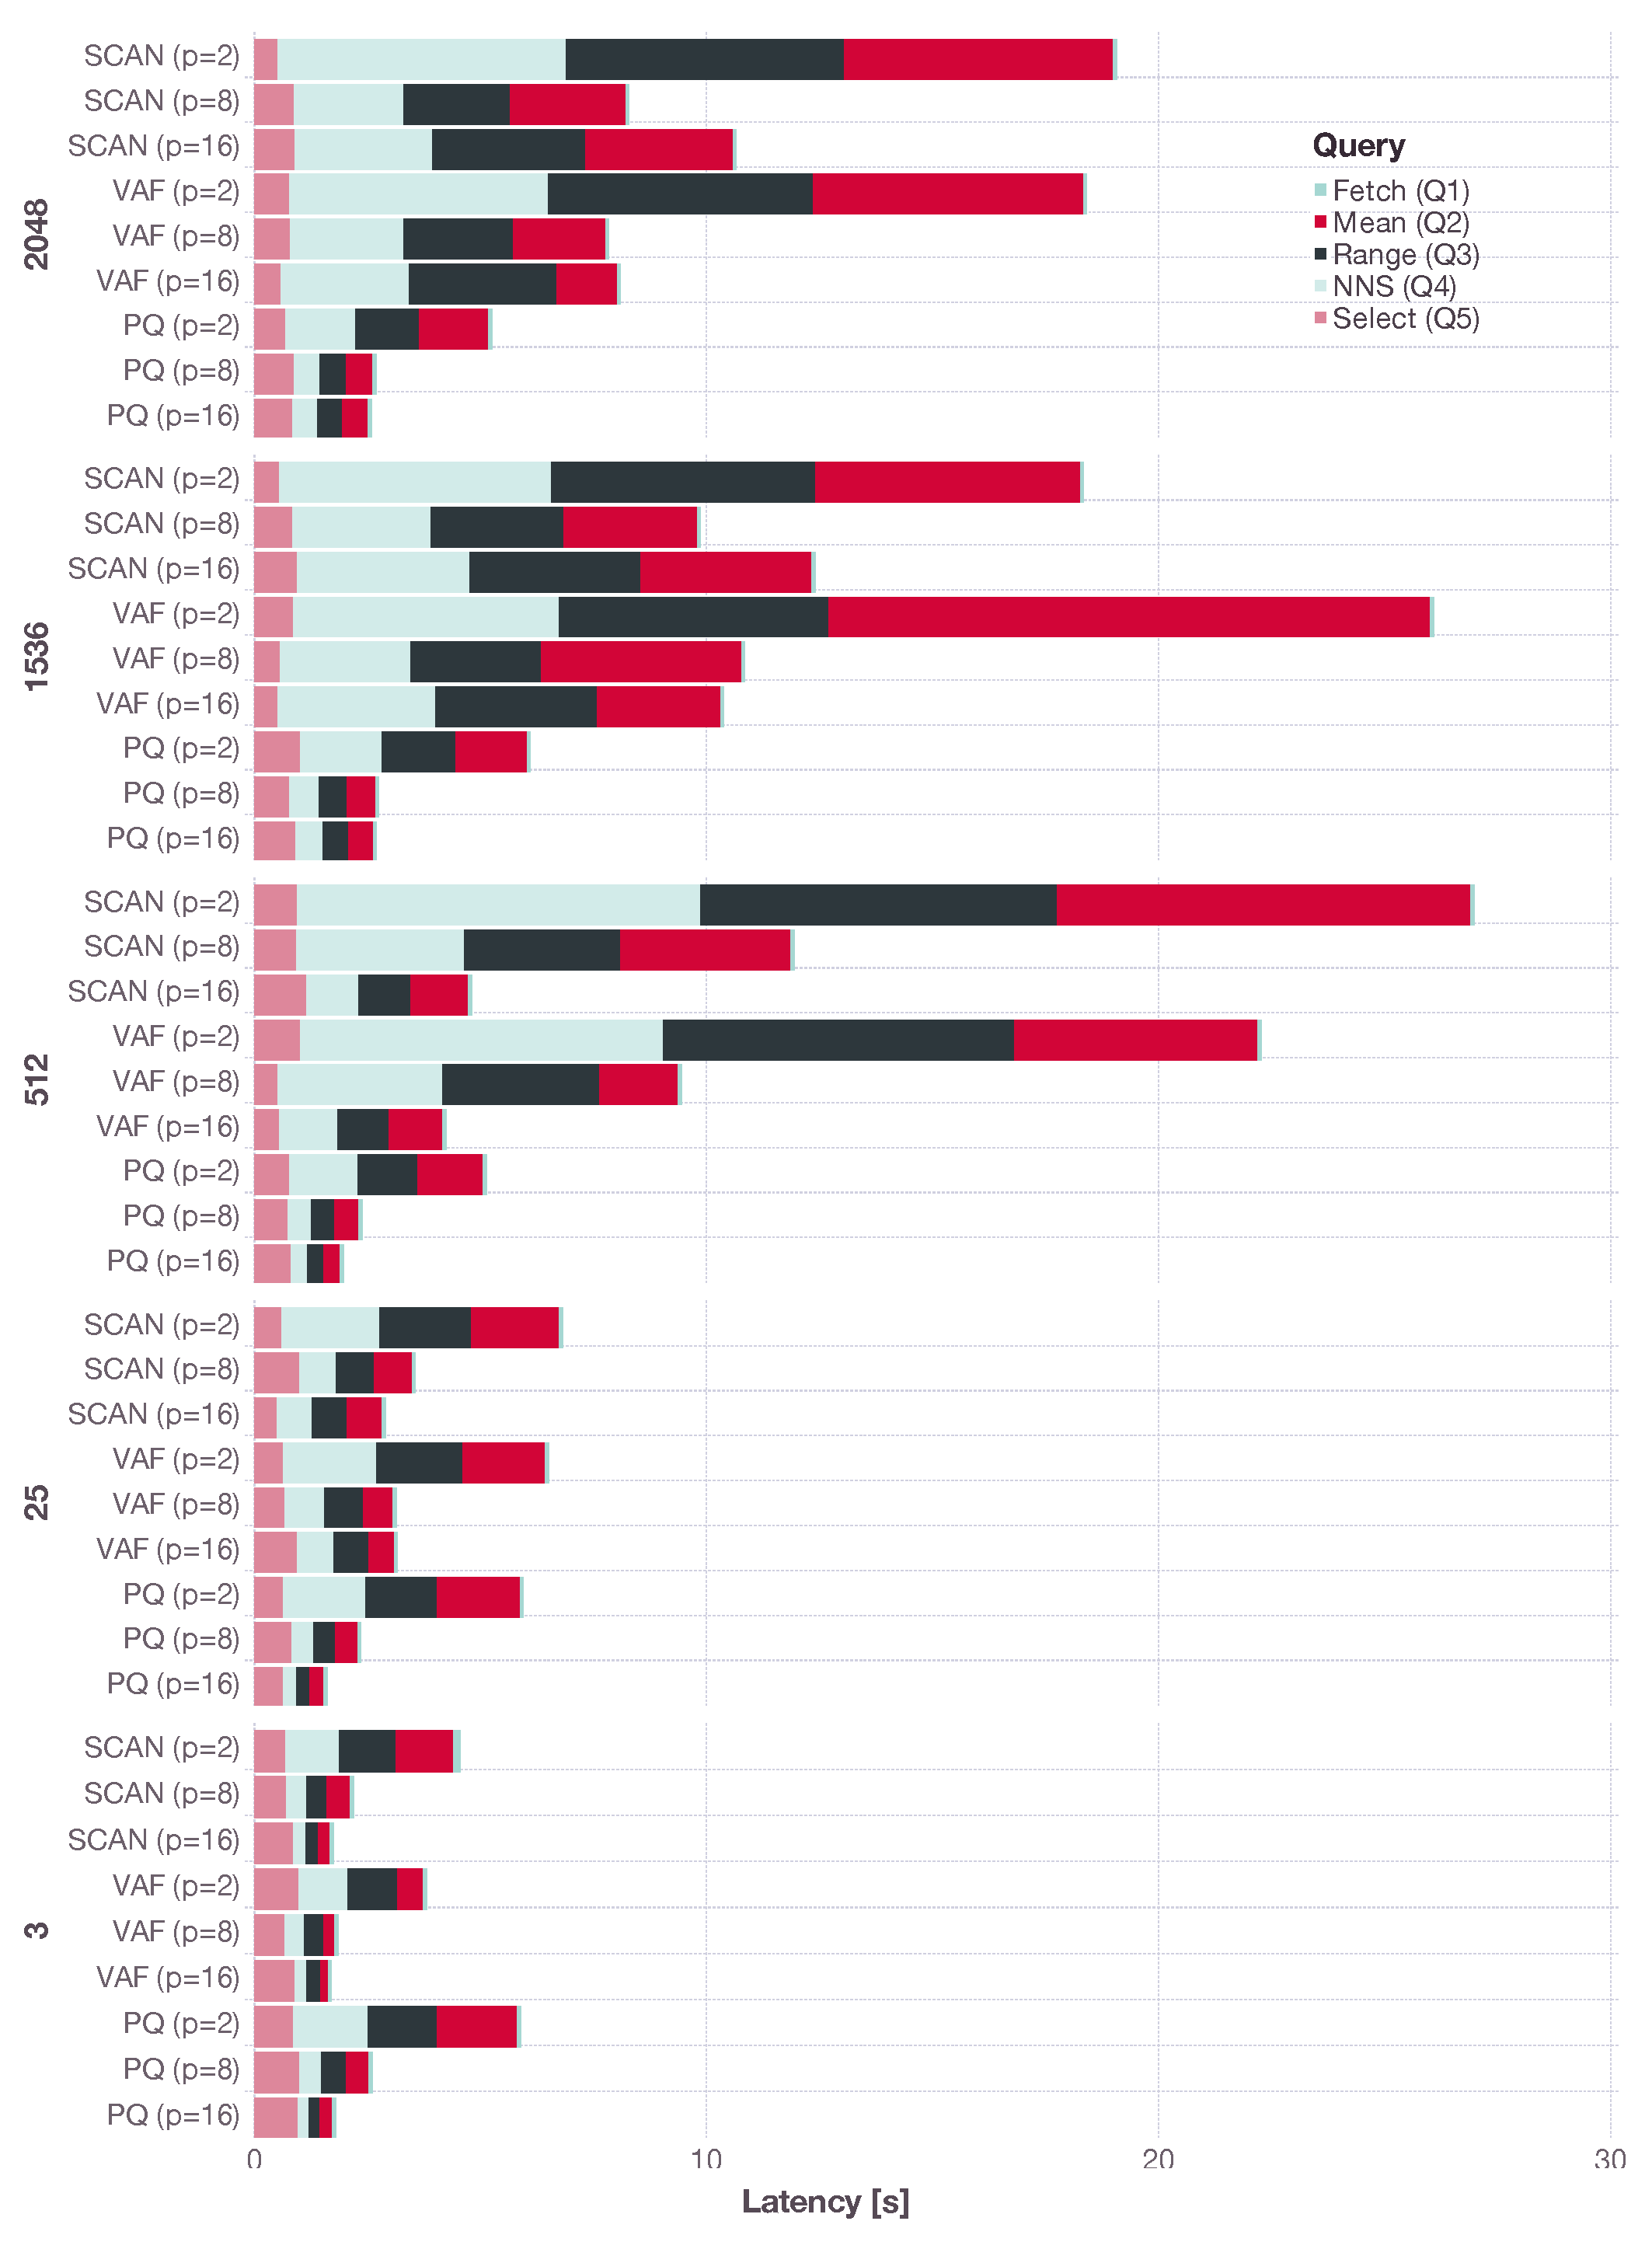
\includegraphics[width=\textwidth]{figures/analytics/analytics-cottontail-runtime}
    \caption {Latency in seconds (x-axis) on different entities using different access methods and levels of parallelisation (y-axis) for the analytics workloads during the first experiment. The individual queries Q1a-Q1e are highlighted in different colours. The use of the \acrshort{vaf} and \acrshort{pq} index was enforced using query hints.}
    \label{figure:analytics_cottontail_runtime}
\end{figure}

\begin{figure}[p]
    \centering
    \begin{subfigure}[b]{\textwidth}
        \centering
        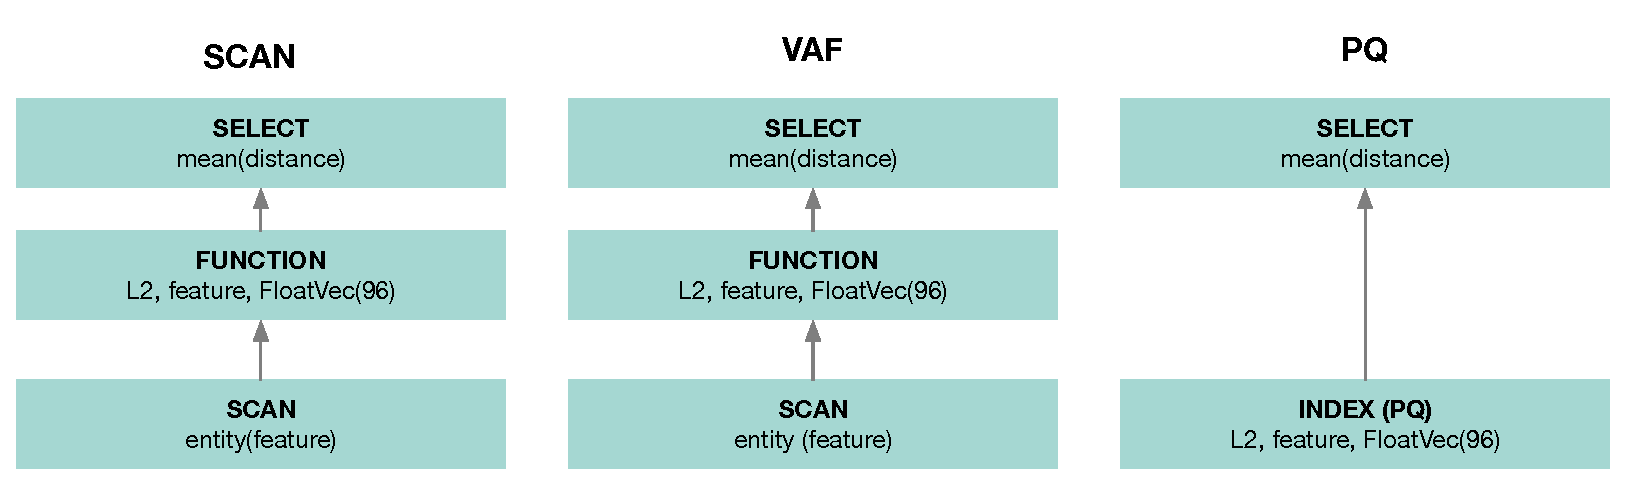
\includegraphics[width=\textwidth]{figures/analytics/query-plan-mean}
        \caption{Execution plans for mean query (Q1b)}
        \label{figure:cottontail_analytics_mean}
    \end{subfigure}
    \hfill
    \centering
    \begin{subfigure}[b]{\textwidth}
        \centering
        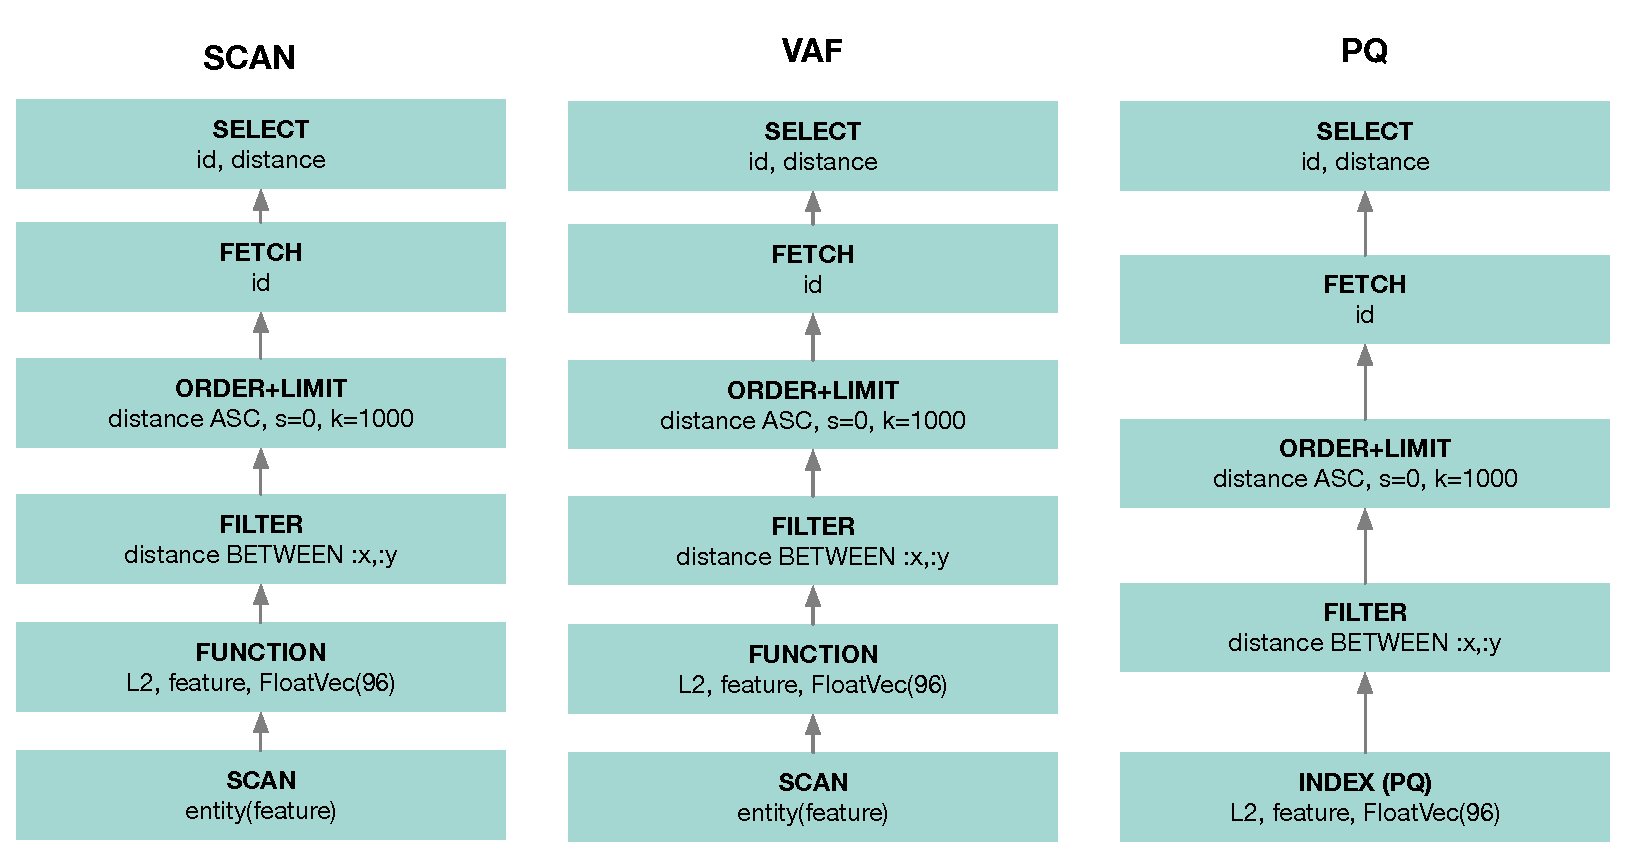
\includegraphics[width=\textwidth]{figures/analytics/query-plan-range}
        \caption{Execution plans for range query (Q1c)}
        \label{figure:cottontail_analytics_range}
    \end{subfigure}
    \hfill
    \centering
    \begin{subfigure}[b]{\textwidth}
        \centering
        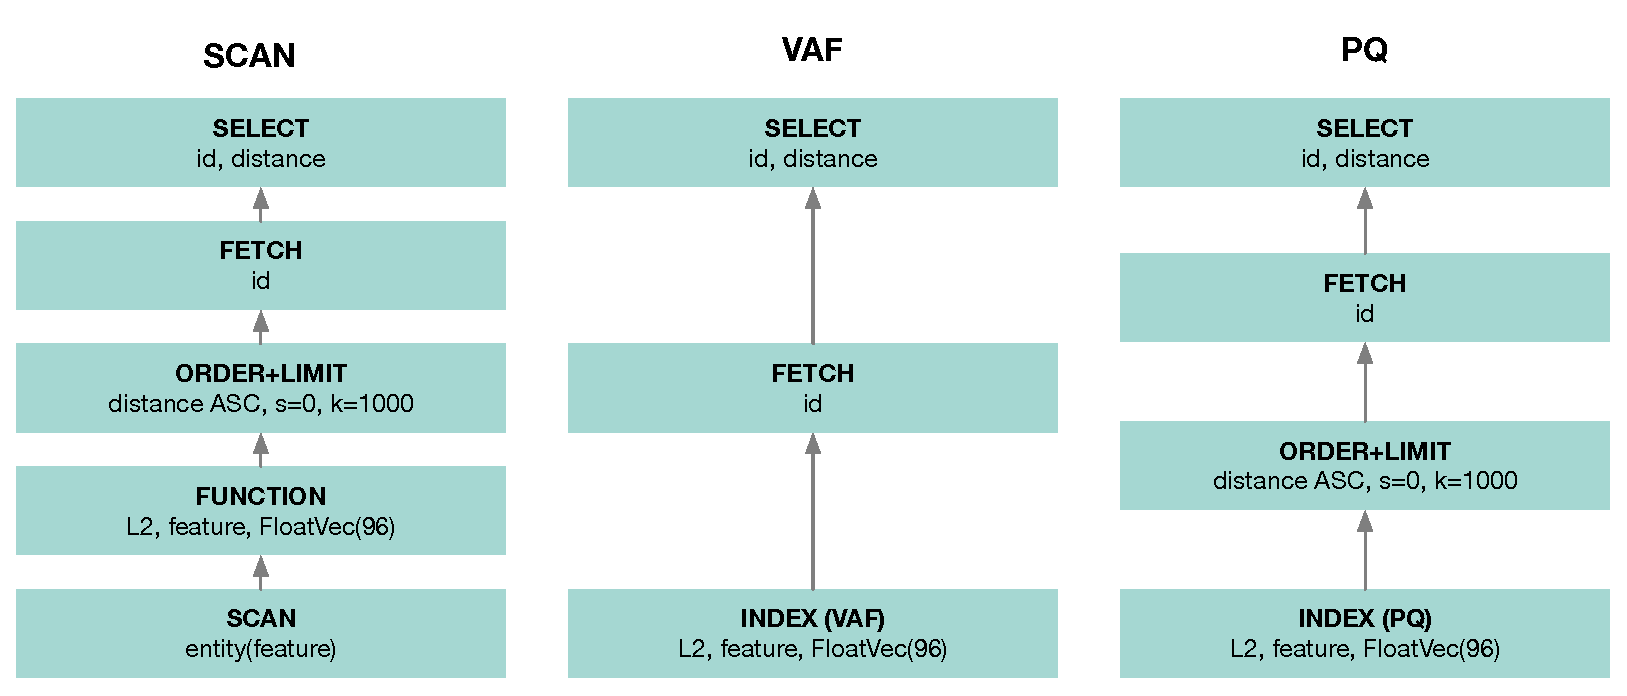
\includegraphics[width=\textwidth]{figures/analytics/query-plan-nns}
        \caption{Execution plans for \acrshort{nns} query (Q1d)}
        \label{figure:cottontail_analytics_nns}
    \end{subfigure}
    \caption{Execution plans produced by \cottontail{} for the mean (Q1b), range (Q1c), and \acrshort{nns} (Q1d) query workloads during the first experiment. The use of the \acrshort{vaf} and \acrshort{pq} index was enforced using query hints.}
    \label{figure:cottontail_analytics_plans}
\end{figure}

An aspect that we would like to draw attention to is the influence of indexes: The Mean (Q1b), Range (Q1c), and \acrshort{nns} (Q1d) queries all seem to benefit from the PQ index, which, according to \Cref{figure:analytics_cottontail_runtime}, provides the lowest latency across all entities and for every degree of parallelisation. This is confirmed when cross-examining the query plans produced by \cottontail{}, which are listed in \Cref{figure:cottontail_analytics_plans}. The plans for the Q1b (\ref{figure:cottontail_analytics_mean}), Q1c (\ref{figure:cottontail_analytics_range}) and Q1d (\ref{figure:cottontail_analytics_nns}) indeed use the \acrshort{pq}, if the respective hint is present. This is possible because \acrshort{pq} can be used to perform a class 1 index replacement (see \Cref{definition:dfc_index_class_1}). 

However, the observed speed-up is traded for a non-negligible, negative impact on quality in terms of recall and \acrshort{ndcg}, as can be seen in \Cref{figure:cottontail_analytics_quality}. Slightly higher values for \acrshort{ndcg} provide us with an indication that mismatches occur further down in the ranking and may therefore be less relevant in practice. What is striking, though, is the very large spread for both recall and \acrshort{ndcg} across all collections, which indicates that the performance of an index is highly dependent on the concrete query vector and thus hard or even impossible to reliably predict. Furthermore, we can observe that the negative impact on quality seems to be larger for range (Q1c, \ref{figure:cottontail_analytics_quality_range}) than for \acrshort{nns} (Q1d, \ref{figure:cottontail_analytics_quality_nns}) queries for both recall and \acrshort{ndcg}. This can be explained by the distortion of the approximate distance as a side-effect of \acrshort{pq}, which has been reported by \cite{Jegou:2010Product} and which is obviously very relevant for range queries. We see this as a confirmation of our proposition, that quality metrics and statistics for the purpose of query planning should be obtained for a type of execution plan rather than globally per index (see \Cref{section:quality_cost_estimation}). Additionally, we can observe that the same index configuration for \acrshort{pq} yields very different results for the different collections. Unfortunately, there does not seem to be an apparent correlation between the dimensionality and the quality of \acrshort{pq} index results, which implies that the quality depends on more than just the size of the vectors.

In contrast, the \acrshort{vaf} index can only provide speed-up for \acrshort{nns} queries (Q1d), since its use is limited to class 3 replacements (see \Cref{definition:dfc_index_class_3}) and the current implementation does not support range queries \footnote{The latter is a limitation of our implementation and could be added, according to \cite{Weber:1998Va}.}. Again, this is confirmed by the query plans shown in \Cref{figure:cottontail_analytics_plans}, where \cottontail{} resorts to a sequential scan in cases where the \acrshort{vaf} cannot be employed. The speed-up gained by using \acrshort{vaf} seems rather small, and it is directly related to the efficiency of the filtering. Over the different runs, we observed \acrshort{vaf} filter efficiency values of between $80\%$ and $99\%$. Again, there seems to be no apparent connection between dimensionality and the effectiveness of the filtering step.

\begin{figure}[tb]
    \centering
    \begin{subfigure}[b]{\textwidth}
        \centering
        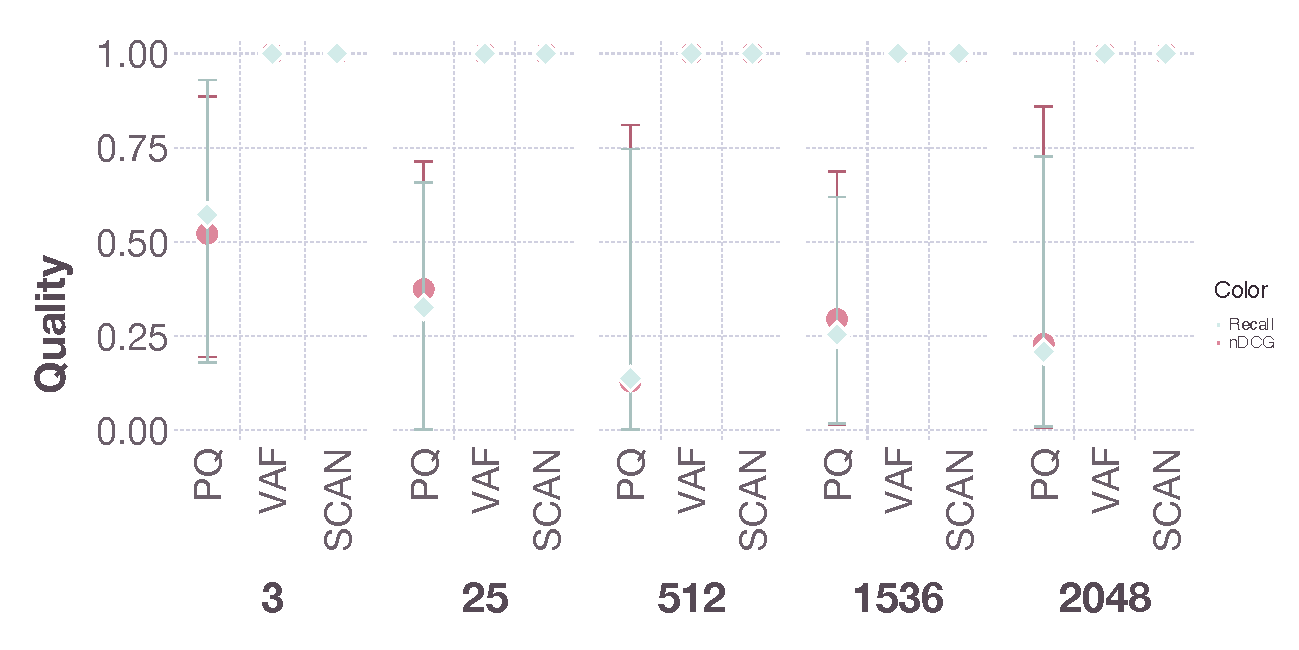
\includegraphics[width=\textwidth]{figures/analytics/analytics-cottontail-quality-range}
        \caption{Quality for range query (Q1c)}
        \label{figure:cottontail_analytics_quality_range}
    \end{subfigure}
    \hfill
    \centering
    \begin{subfigure}[b]{\textwidth}
        \centering
        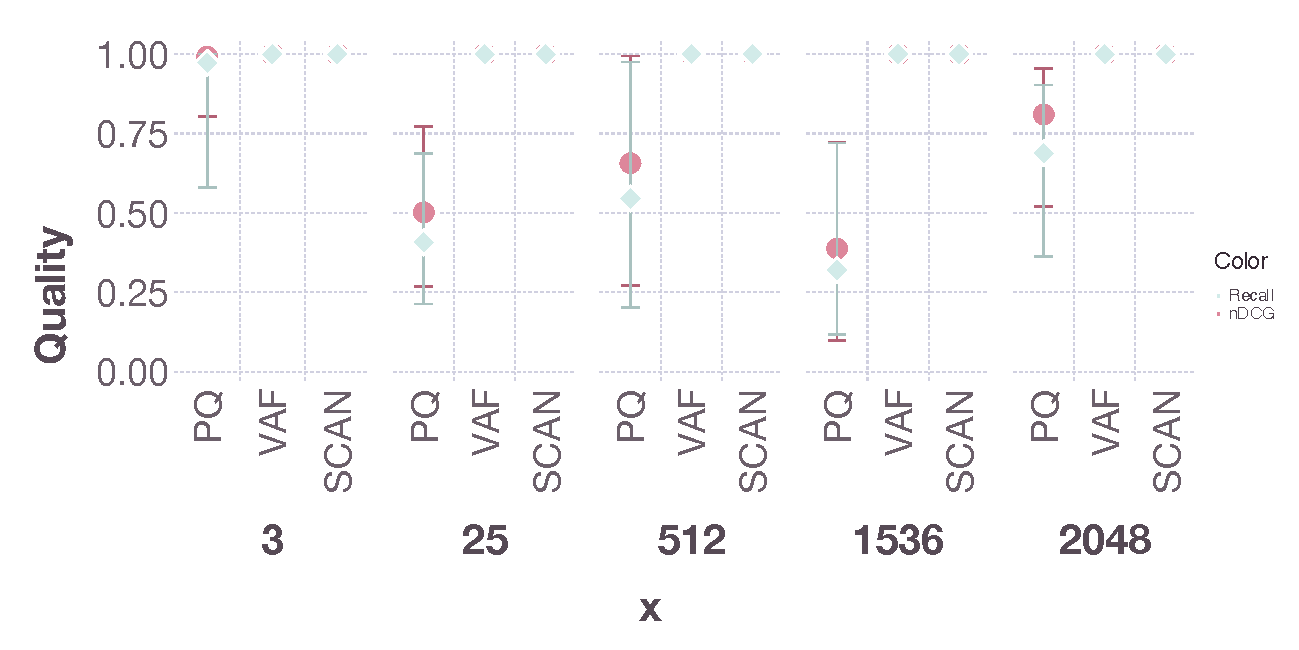
\includegraphics[width=\textwidth]{figures/analytics/analytics-cottontail-quality-nns}
        \caption{Quality for \acrshort{nns} query (Q1d)}
        \label{figure:cottontail_analytics_quality_nns}
    \end{subfigure}
    \caption{Quality of results (x-axis) in terms of recall (mint) and \acrshort{dcg} (red) on different entities using different access methods (y-axis) for the range (Q1c) and \acrshort{nns} (Q1d) query workloads during the first experiment. The use of the \acrshort{vaf} and \acrshort{pq} index was enforced using query hints.}
    \label{figure:cottontail_analytics_quality}
\end{figure}

We must assume, that the quality of all the tested index structures can be fine-tuned by choosing appropriate values for the hyperparameters. Since these values seem to depend on a multitude of factors (e.g., collection size, distribution of the data, dimensionality), this may not be a straightforward undertaking. However, learning an optimal set of hyperparameters for a given collection and index  could be an interesting research direction for the future, very similar to learned index structures proposed by \cite{Kraska:2018Case}.

\subsection{Experiment 2: Influence of Cost Policy}
\label{section:cost_model_evaluation}

So far, we have forced \cottontail{} into using one index over another by providing query hints that make an explicit choice. For this second experiment, we delegate the decision to \cottontail{} and observe how changing parameters in the cost policy influence plan selection. The idea behind the cost policies was explained in \Cref{section:cost_model}. Basically, they assign weight to the parameters of the cost model -- the cost of IO, CPU, memory use, and reduction in quality -- and can be used to steer the planner's behaviour depending on the use-case. For the experiment, we fixed the values of $w_{\mathtt{CPU}} = 0.3$, $w_{\mathtt{IO}} = 0.6$, and $ w_{\mathtt{MEM}} = 0.1$ (\cottontail{}'s default values) via the respective query hint. We then used the \texttt{EXPLAIN} endpoint to generate and print the execution plans as we increased the weight of the quality parameter $w_{\mathtt{Q}}$ from $0.1$ to $0.9$ in steps of $0.1$. The results are depicted separately for the mean (Q1b, \ref{figure:cottontail_analytics_cost_mean}), range (Q1c, \ref{figure:cottontail_analytics_cost_range}), and \acrshort{nns} (Q1d, \ref{figure:cottontail_analytics_cost_nns}) queries, for which we plot the scores and the ranking assigned to the individual plans by \cottontail{}'s query planner. Furthermore, we visualise all query execution plans that appear in the top three ranks.

\begin{figure}[tb]
    \centering
    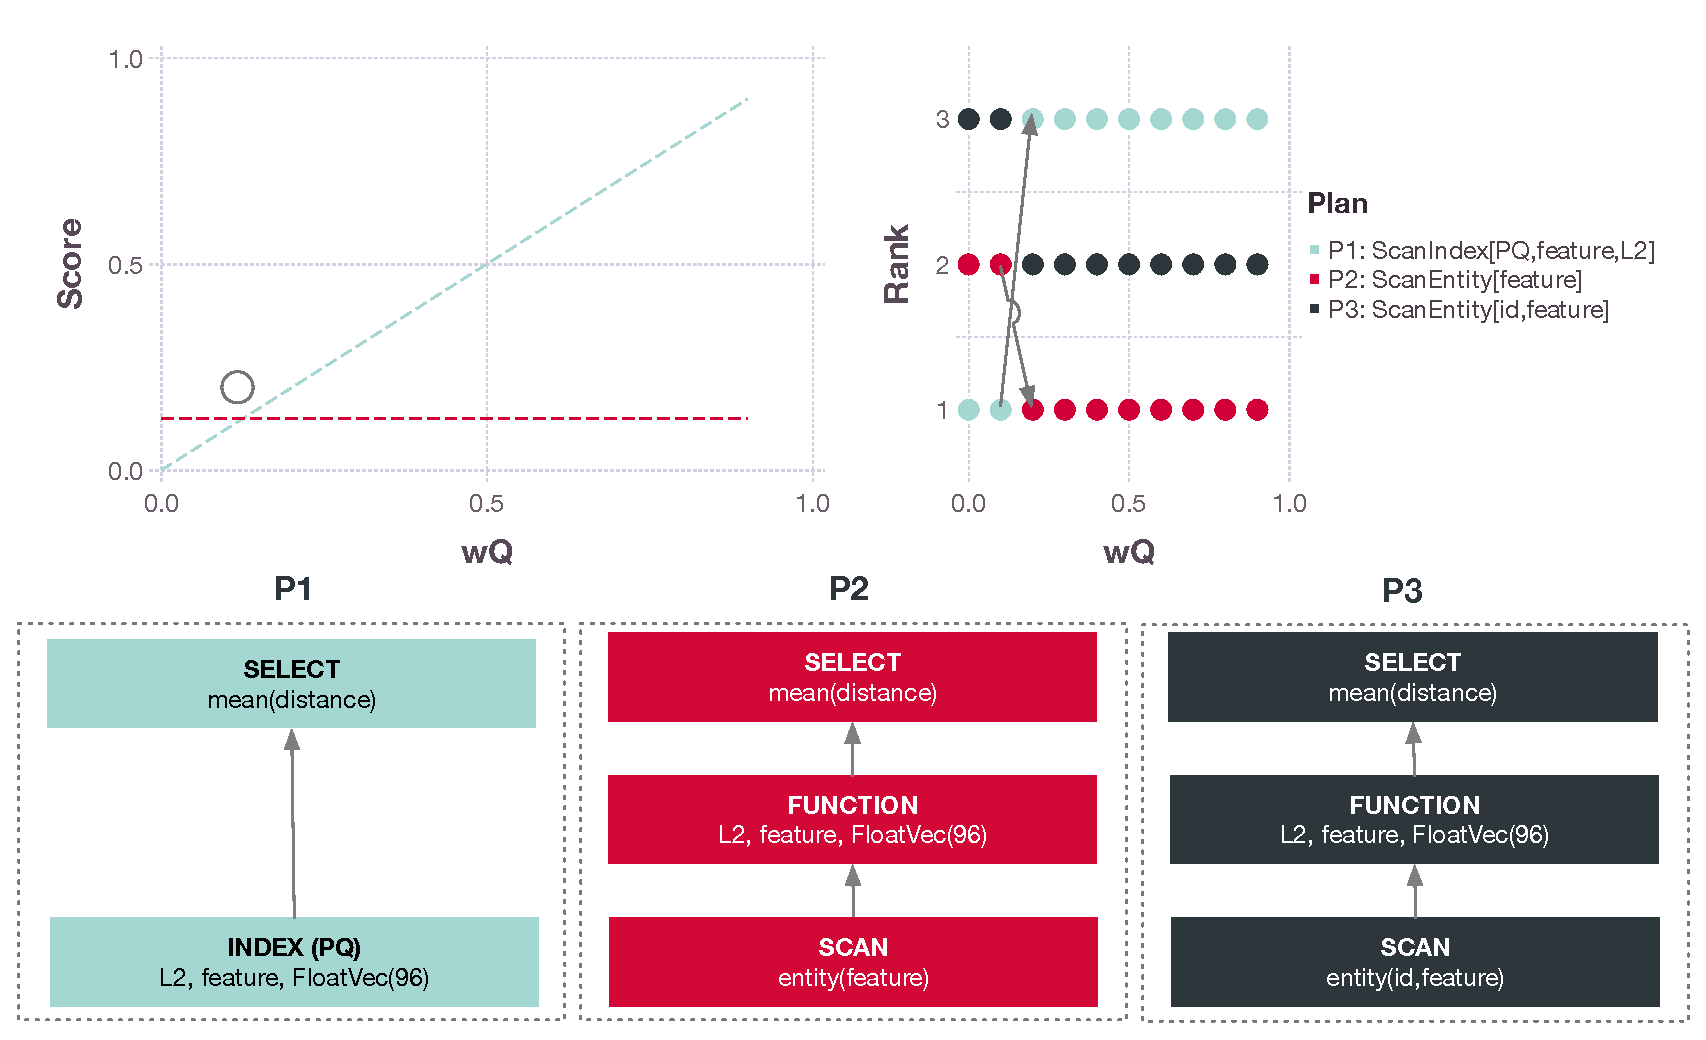
\includegraphics[width=\textwidth]{figures/analytics/analytics-cottontail-cost-mean-annotated}
    \caption{Score and rank of different query plan options for the mean query (Q1b). The preferred option for $w_{\texttt{Q}} = 0.0$ involves the scan of a \acrshort{pq} index. As $w_{\texttt{Q}}$ goes up, the cost of impaired quality increases and a full entity scan ($P_2$) takes over, since none of the available indexes can satisfy the query. The scores for $P_2$ and $P_3$ do not depend on the quality parameter and incur almost the same cost, with $P_2$ being the less expensive variant.}
    \label{figure:cottontail_analytics_cost_mean}
\end{figure}

For Q1b (\Cref{figure:cottontail_analytics_cost_mean}) we see that at least three different options exists and that by default, i.e., for $w_{\mathtt{Q}} = 0.0$, the option involving the \acrshort{pq} index ($P_1$) is favoured. This is consistent with the findings from our first benchmark, where we demonstrated that \acrshort{pq} is the fastest of the available options. As long as the quality weight parameter is low ($w_{\mathtt{Q}} \in [0.1, 0.2]$), $P_1$ remains the plan with the lowest score and thus the selected candidate. As $w_Q$ increases, the score of $P_1$ increases as well and it moves up in the ranking, and plan $P_2$, which involves a full table scan, takes over the lead. The two alternatives $P_2$ and $P_3$ are almost equivalent with the only difference that $P_3$ includes the \texttt{id} column in the initial scan, which is not required to calculate the mean and can therefore be optimised out (the application of the deferral rules described in \Cref{section:cottontail_query_planner}). Consequently, $P_3$ is slightly more expensive and $P_2$ is selected instead. 

\begin{figure}[p]
    \centering
    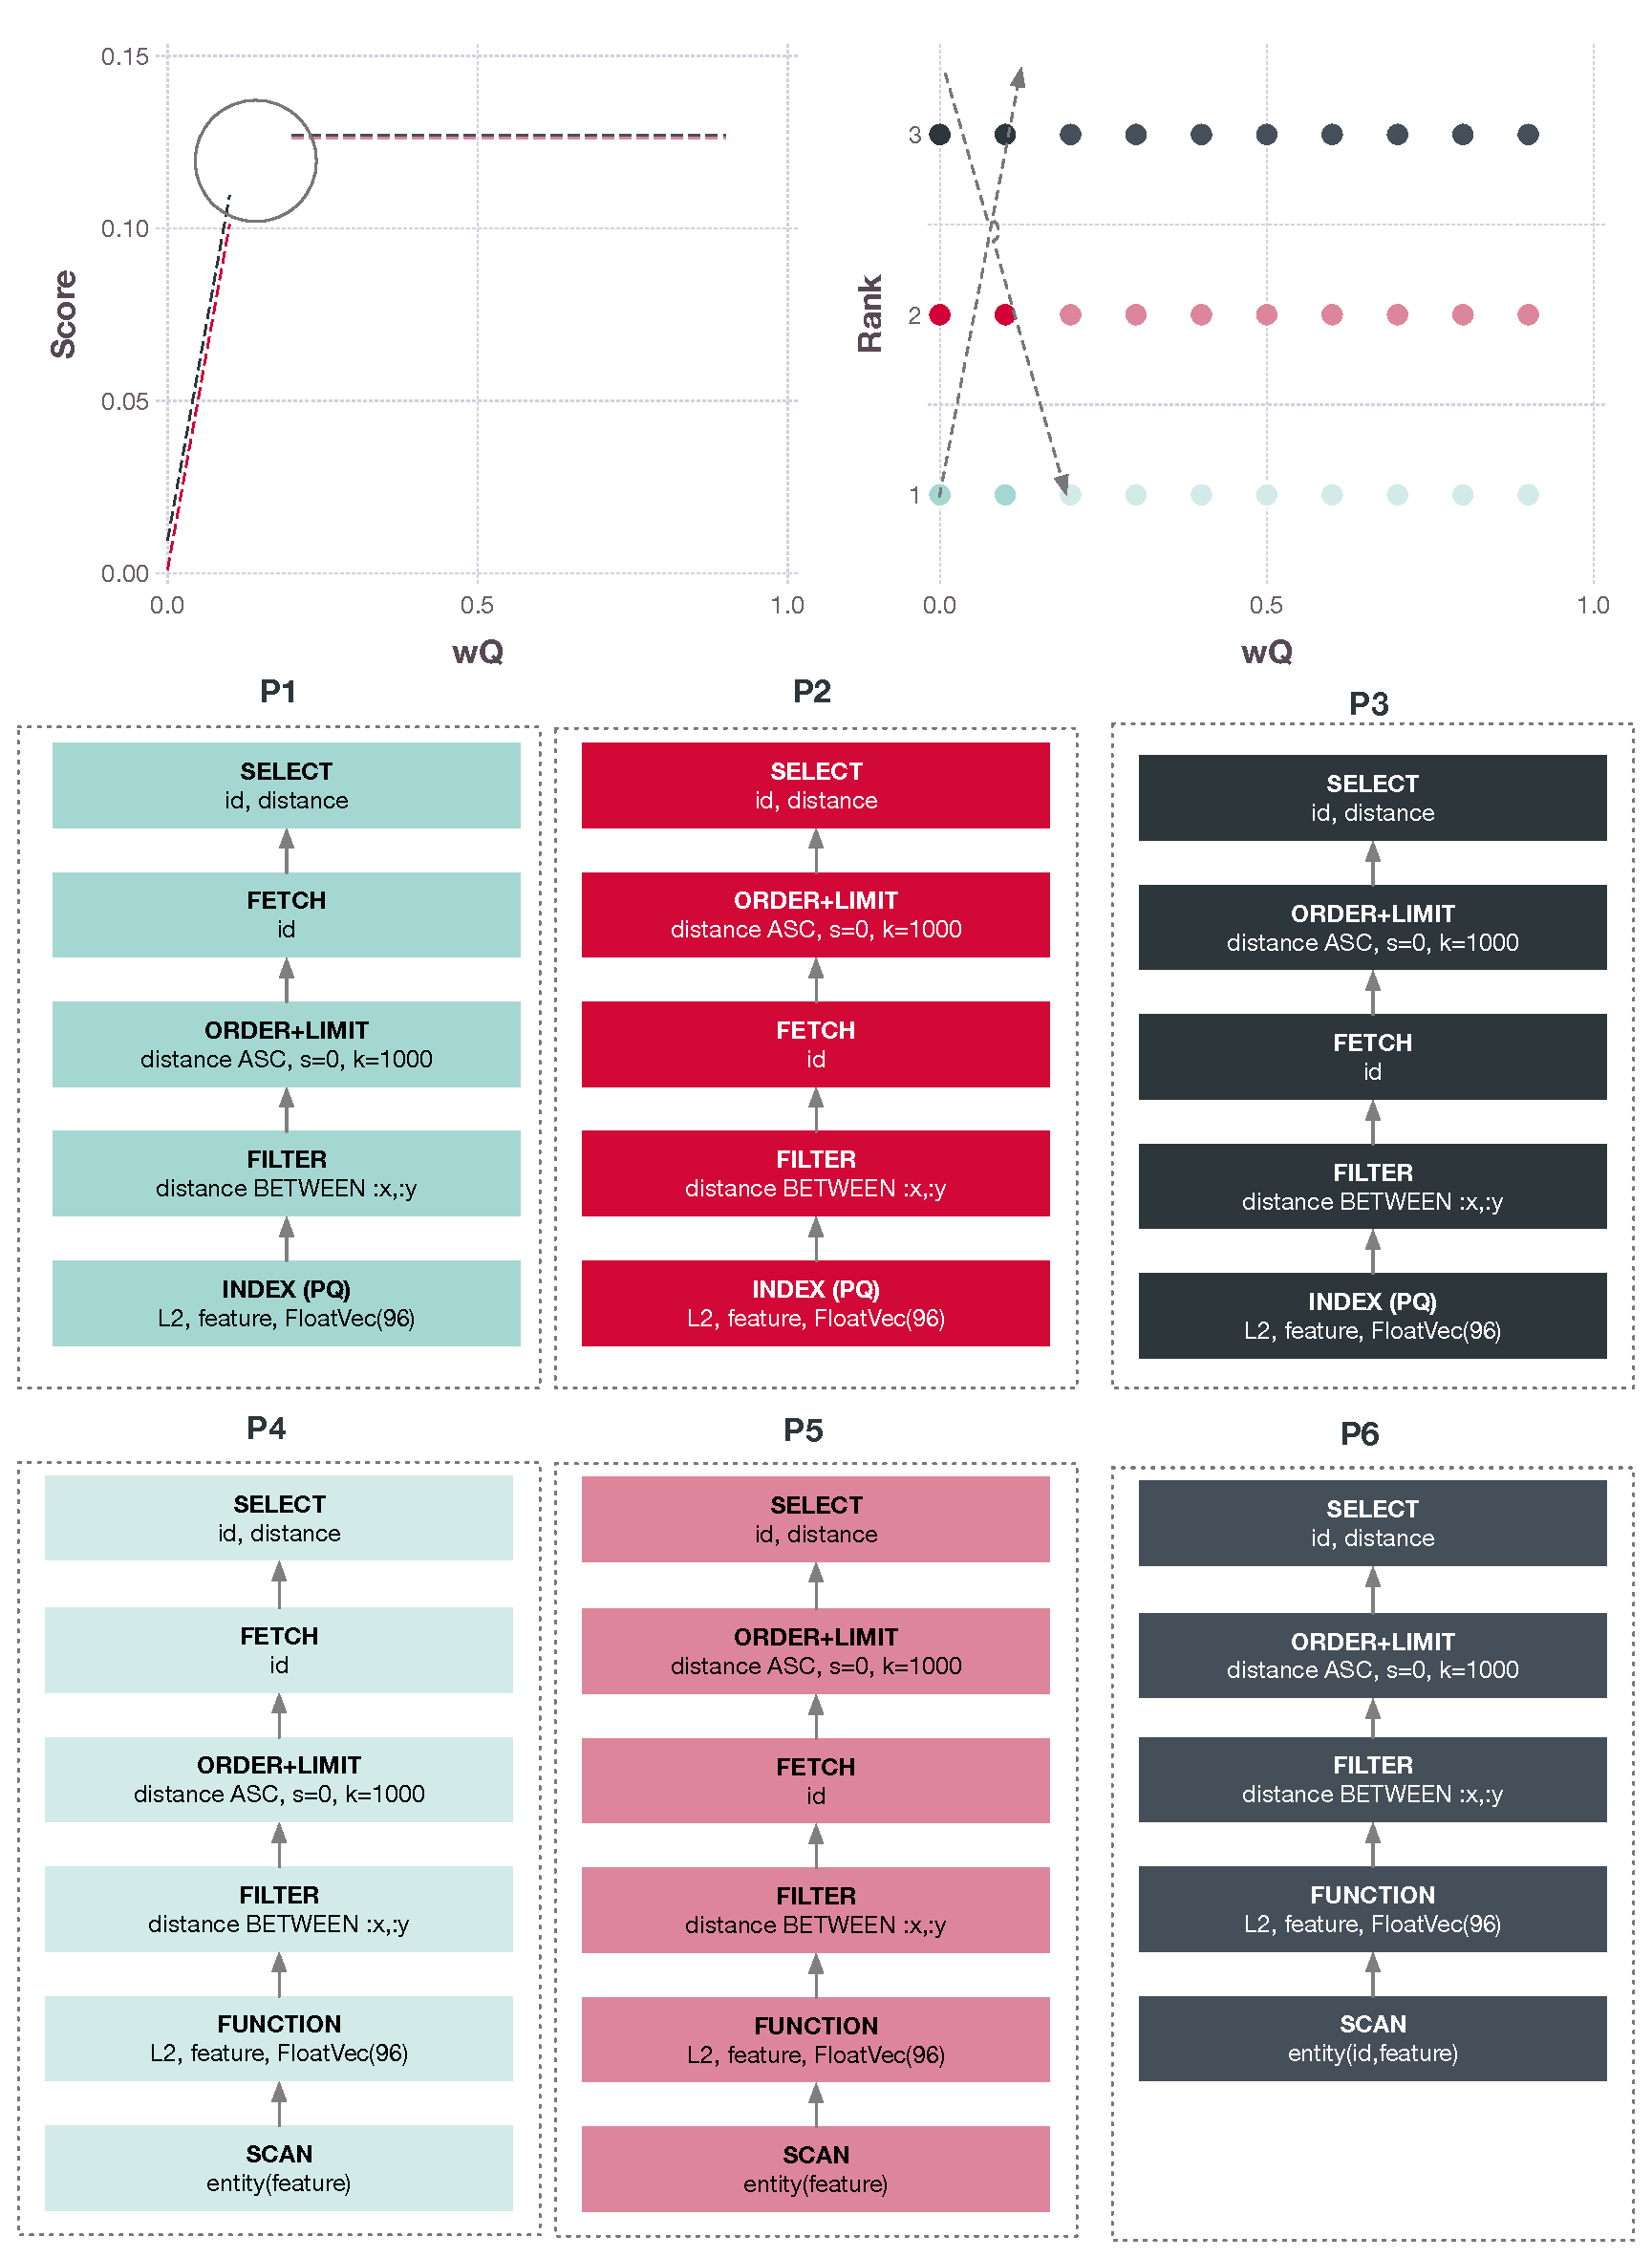
\includegraphics[width=\textwidth]{figures/analytics/analytics-cottontail-cost-range-annotated}
    \caption{Score and rank of different query plan options for the range query (Q1c). The preferred option for $w_{\texttt{Q}} = 0.0$ involves the scan of a \acrshort{pq} index. As $w_{\texttt{Q}}$ goes up, the cost of impaired quality increases and a full entity scan takes over, since none of the available indexes can satisfy the query. The scores for $P_4$ through $P_6$ do not depend on the quality parameter and incur almost the same cost, with $P_4$ being the least expensive.}
    \label{figure:cottontail_analytics_cost_range}
\end{figure}

\begin{figure}[p]
    \centering
    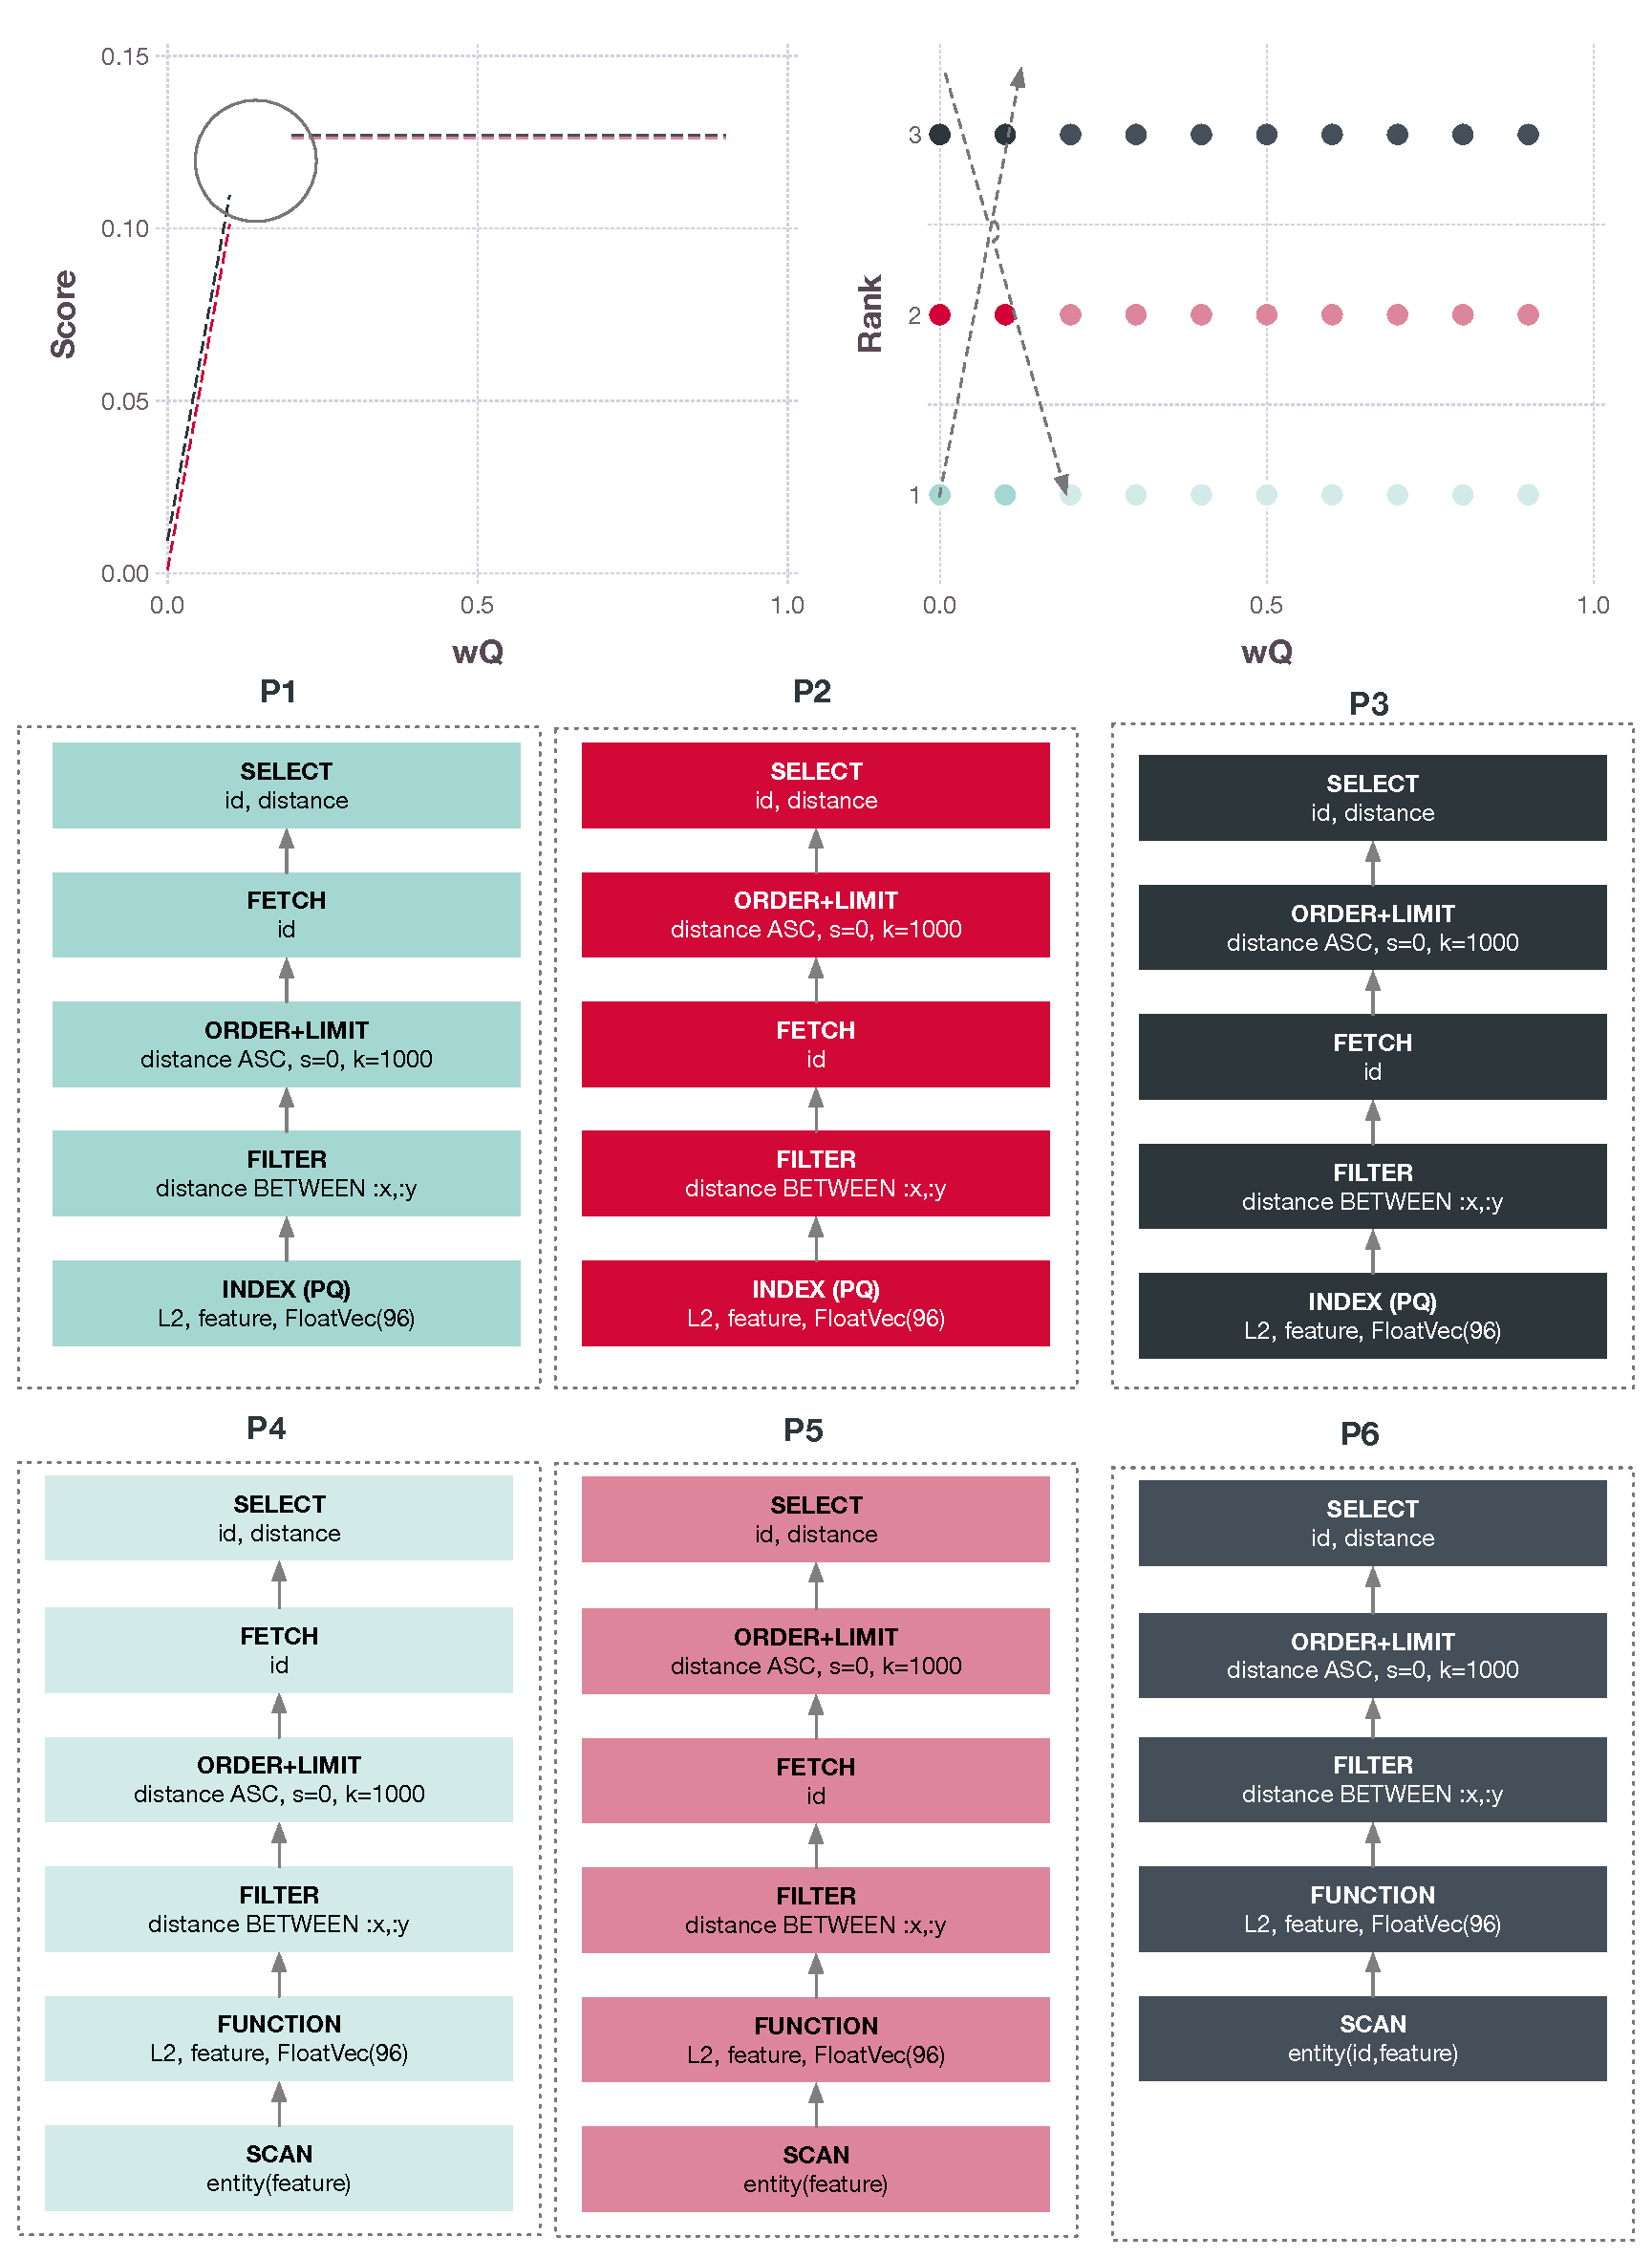
\includegraphics[width=\textwidth]{figures/analytics/analytics-cottontail-cost-nns-annotated}
    \caption{Score and rank of different query plan options for the \acrshort{nns} query (Q1d). The preferred option for $w_{\texttt{Q}} = 0.0$ involves the scan of a \acrshort{pq} index. As $w_{\texttt{Q}}$ goes up, the cost of impaired quality increases and a \acrshort{vaf} index scan ($P_3$) takes over, which can also satisfy \acrshort{nns} queries. Since \acrshort{vaf} does not incur quality costs, it remains the favoured option.}
    \label{figure:cottontail_analytics_cost_nns}
\end{figure}

A very similar behaviour can be observed for Q1c (\Cref{figure:cottontail_analytics_cost_range}). Over the course of the measurements, six options appear in the top three ranks. Again, we start with  $w_{\mathtt{Q}} = 0.0$, where $P_1$ is the fastest option and again, it involves a scan of the \acrshort{pq} index. $P_2$ and $P_3$ are different variants involving the same index scan but use different intermediate operations and therefore differ in the fetching of required columns and sort algorithms (application of the deferral and implementations rules described in \Cref{section:cottontail_query_planner}). As $w_Q$ increases, $P_1$, $P_2$, and $P_3$ disappear from the top three ranks, since all three plans use the same index and therefore result in impaired quality. $P4$ -- which is the query plan involving the evaluation of a full entity scan -- takes over and keeps the lowest rank. Again, $P5$ and $P6$ are less optimal variants of $P4$ and are therefore not considered.

For both Q1b and Q1c using \acrshort{pq} or a full entity scan were the only available options due to the constraints discussed in \Cref{section:dfc_and_indexes}. For Q1d (\Cref{figure:cottontail_analytics_cost_nns}) we see a third option appear, which is the use of a \acrshort{vaf} index ($P3$). As $w_{\mathtt{Q}}$ exceeds $0.1$, the scan of the \acrshort{vaf} index becomes the preferred choice and $P_1$ and $P_2$ become the second and third options. As $w_{\mathtt{Q}}$ moves beyond $0.2$, $P_1$ and $P_2$ disappear from the top 3 and the entity scan becomes the preferred alternative to the \acrshort{vaf} index scan. However, since the \acrshort{vaf} index does not incur quality cost, it remains the favoured option.

\newpage

\subsection{Benchmark 3: Influence of Optimisation}
We have demonstrated in the first experiment, that high-dimensional index selection has a considerable impact on query execution performance. However, as described in \Cref{chapter:cottontaildb}, in addition to selecting indexes, the query planner also performs other optimisations of the plan before executing it. For this experiment, we completely bypassed plan optimisation and observed the execution time for an unoptimised plan -- which is a naive implementation of the canonical operator tree. All experiments were performed with parallelisation switched off, i.e., single-threadedly. The results are depicted in \Cref{figure:cottontail_analytics_optimisation}.

\begin{figure}[p]
    \centering
    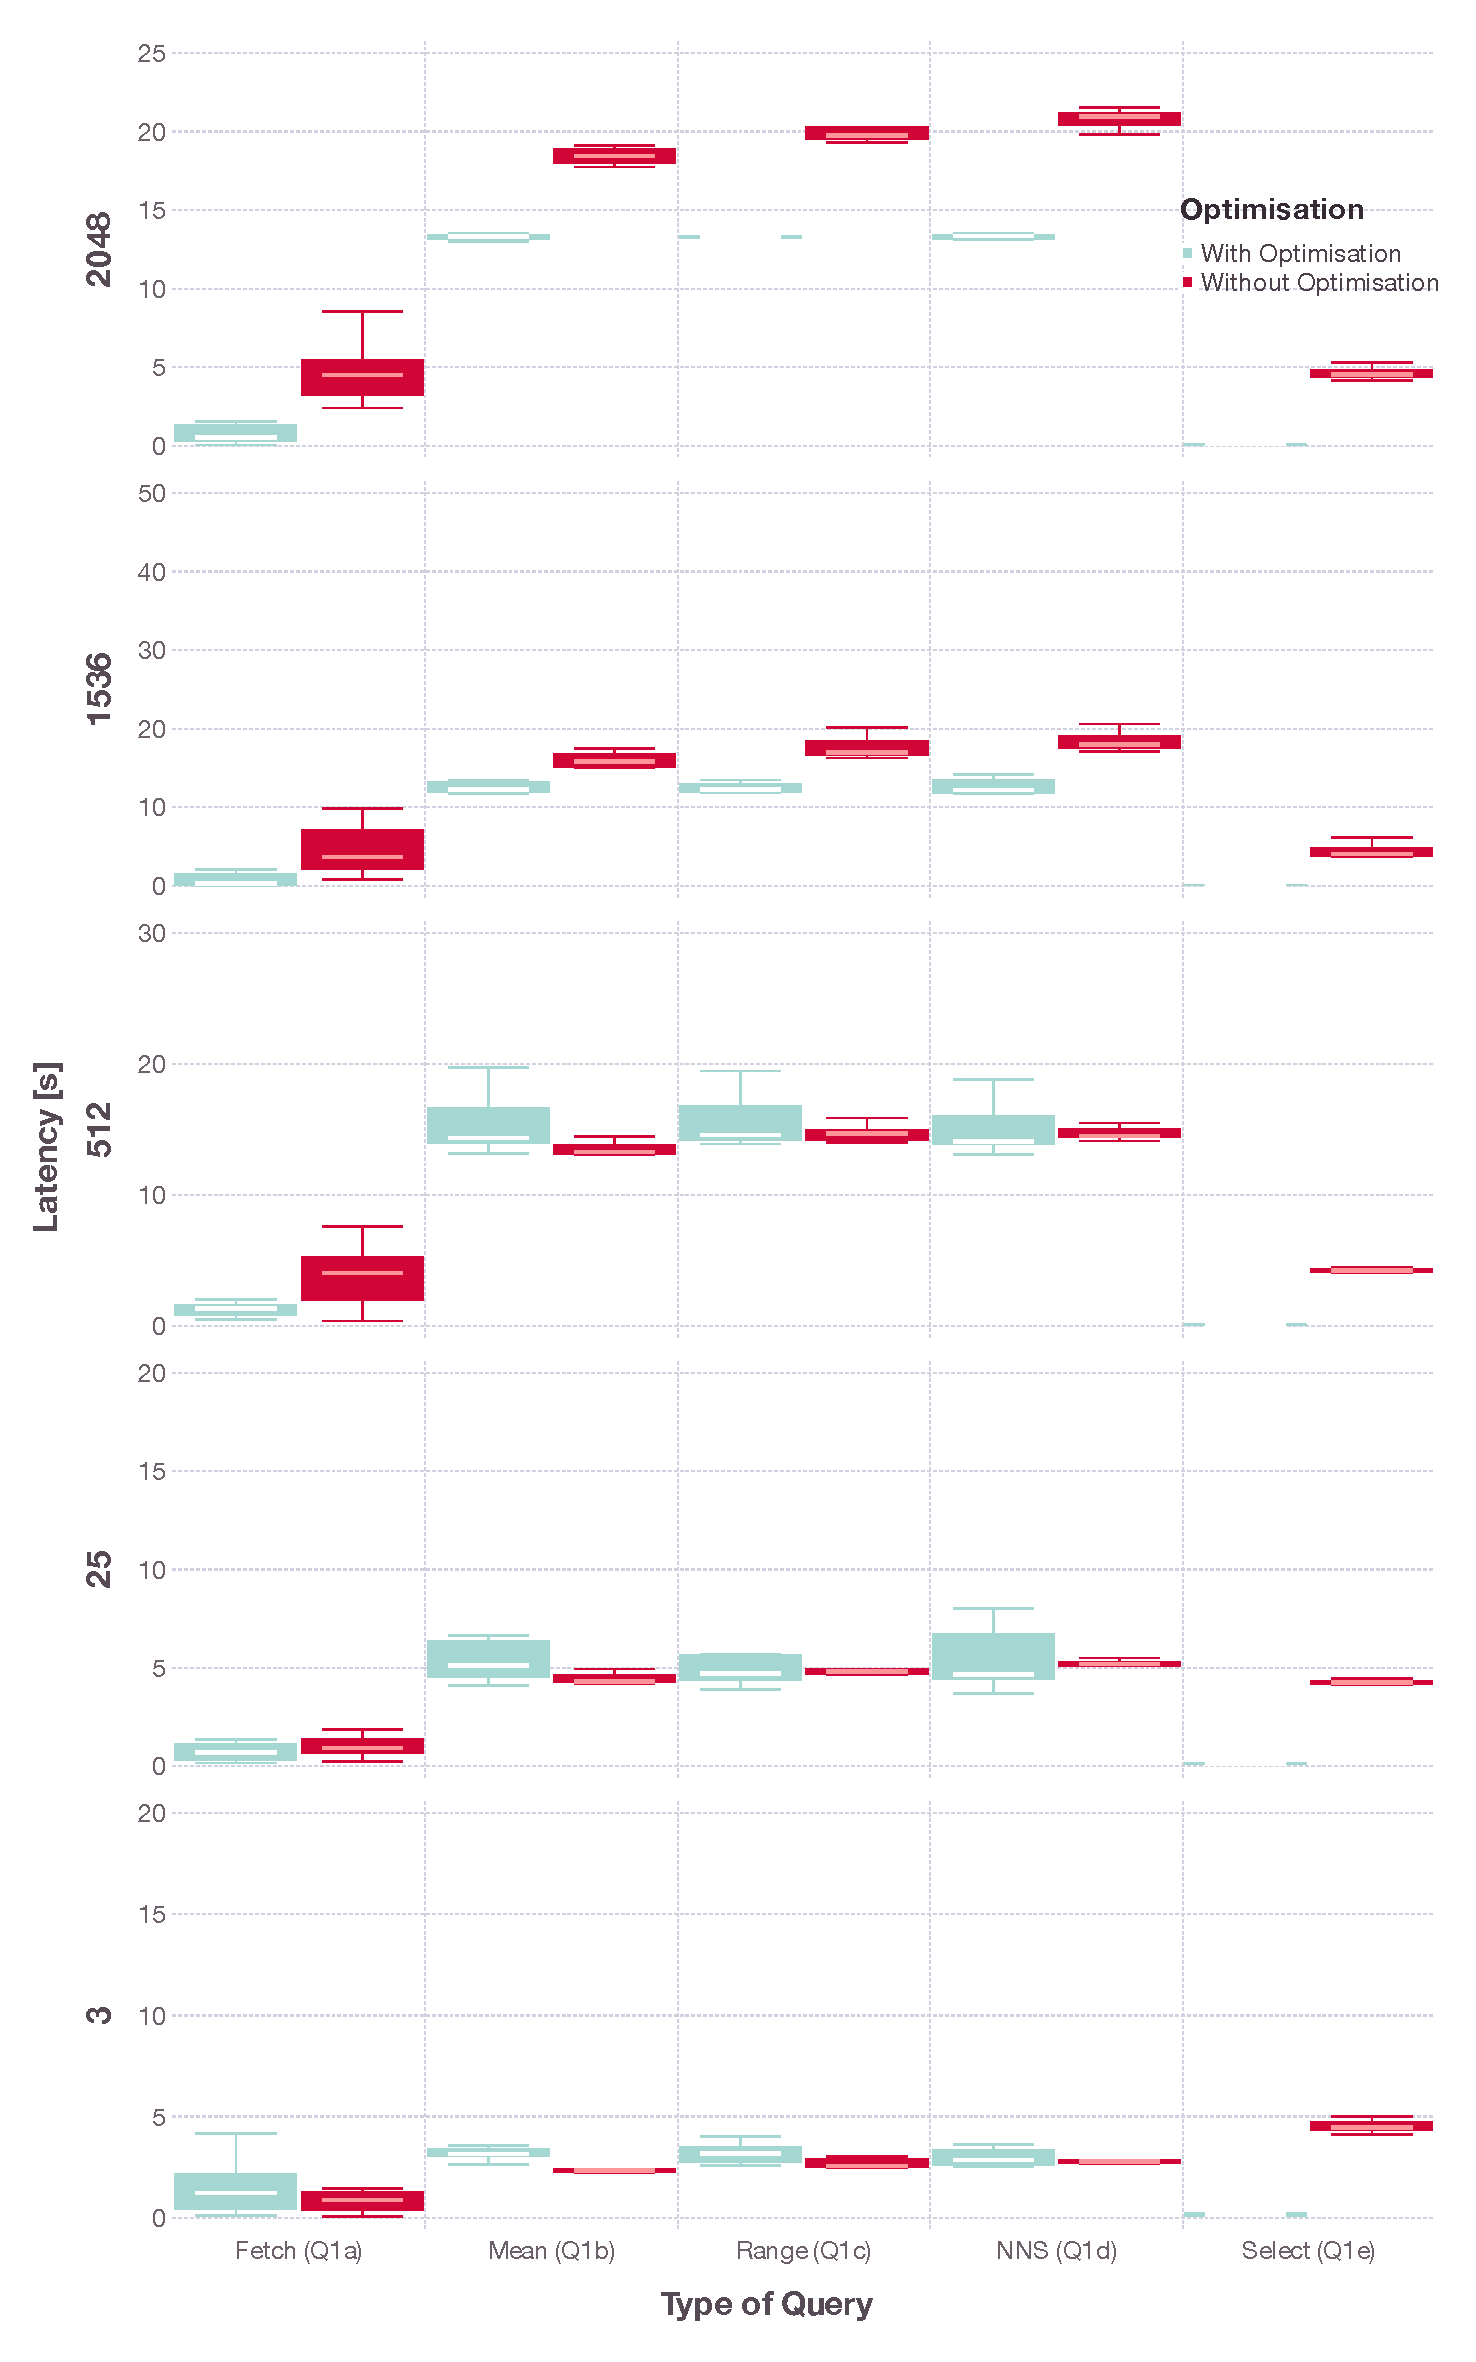
\includegraphics[width=\textwidth]{figures/analytics/analytics-cottontail-optimisation-runtime}
    \caption{Latency in seconds on different collections (y-axis) for the query workloads Q1a through Q1e (x-axis) with (mint) and without (red) query optimisation.}
    \label{figure:cottontail_analytics_optimisation}
\end{figure}

We can see from this graph, that optimisation seems to have a larger effect on latency for proximity-based queries (Q1b to Q1d) involving high-dimensional vectors than it does for low dimensional ones. However, optimisation also seems to introduce a larger variance in latency, making it less predictable. Both effects can be attributed to the column-access deferral optimisation rule, which pushes access to columns that are not required for query execution up in the tree until after a ($s,k$-)selection has been executed. The idea is to reduce or even avoid access to data that is not needed and therefore the number of \acrshort{io} operations. This optimisation seems to be highly relevant for large vectors, but it diminishes as dimensionality decreases. We suspect that the page cache, which -- given the huge amount of memory available -- can keep many of the requested pages in memory, is responsible for this behaviour. When larger entities are being scanned, the cache becomes more saturated, and the likelihood of a cache miss becomes higher resulting in a higher overall latency. This effect is of course amplified if more than one column is being scanned, as in the unoptimised case.

As a second observation, we see that optimisation consistently benefits the Select (Q1e) query, where we load segment entries that match the preceding query results. The explanation of this is as simple as it is unexciting: The select query (Q1e) benefits from a $B^{+}$-tree index scan in the optimised case, while the unoptimised case uses a full entity scan. Last but not least, we see that the impact of optimisation is slightly larger for range (Q1c) and \acrshort{nns} (Q1d) queries than it is for the mean query. This can be attributed to a second optimisation, which combines the sorting and limiting used for Q1c and Q1d into a single step that uses a specialised heap data structure. This sort algorithm can be executed more efficiently and uses less memory than naive sorting. We expect the impact to be even larger for setups that do not have the same amount of memory and must therefore resort to on-disk sorting.

\newpage

\section{Large-Scale Similarity Search}
This experiment is a direct comparison of Milvus and \cottontail{} and is about mere performance. We execute all queries on prepared shards of the Deep1B \cite{Babenko:2016Efficient} dataset ($d=96$), with $k=1000$ using different execution strategies and compare the obtained metrics. The shards contain 5 million, 10 million, 100 million and 1 billion $96$-dimensional \texttt{float} vectors and are stored in dedicated collections (Milvus) or entities (\cottontail). The three types of queries are:
\begin{enumerate*}[label=(\roman*),itemjoin={{, }}, itemjoin*={{, and, }}, after={{.}}]
    \item A simple \acrshort{nns} query that only returns the primary key and the distance (Q2a)
    \item a \acrshort{nns} query that additionally returns the query vector (Q2b)
    \item a \acrshort{nns} query with a Boolean filter (Q2c, hybrid query in Milvus terminology)
\end{enumerate*} 
The Pseudo-SQL is provided in \Cref{listing:big_nns_query}. We use the query vectors provided with the Deep1B dataset and establish a ground truth by executing a brute-force search.

\begin{lstlisting}[language=SQL, caption={Pseudo-SQL of the queries executed for this measurement.}, label=listing:big_nns_query, numbers=none]
    /* Q2a: Simple NNS without feature vectors. */
    select id, euclidean(feature, <query>) as dst from <collection> order by dst limit 1000
    
    /* Q2b: NSS that returns feature vectors. */
    select id, feature, euclidean(feature, <query>) as dst from <collection> order by dst limit 1000

    /* Q2c: Hybrid query without feature vector. */
    select id, euclidean(feature, <query>) as dst from <collection> where category = <category> order by dst limit 1000
\end{lstlisting}

\subsection{\cottontail}
\label{section:evaluation_bignns_cottontail}
For this benchmark, we prepared a selection of indexes on the respective entities in \cottontail{}: Two variants of a \acrshort{pq} index, one organised as a list for exhaustive search ($8$ subspaces, $256$ centroids) and one organised as an inverted list for approximate search ($8$ subspaces, $256$ centroids and $256$ coarse centroids) and a \acrshort{vaf} index. Furthermore, we created a $B^{+}$-Tree index on the column \texttt{categories}, which we expect to be beneficial for Boolean search. We again use query hints to nudge \cottontail{} into using certain high-dimensional index structures to be able to compare the different query execution strategies. Across all workloads, we compare the performance of four different types: Sequential scan and the scan of the \acrshort{vaf} and the (IVF-)\acrshort{pq} indexes.

\begin{landscape}
    \begin{figure}[p]
        \centering
        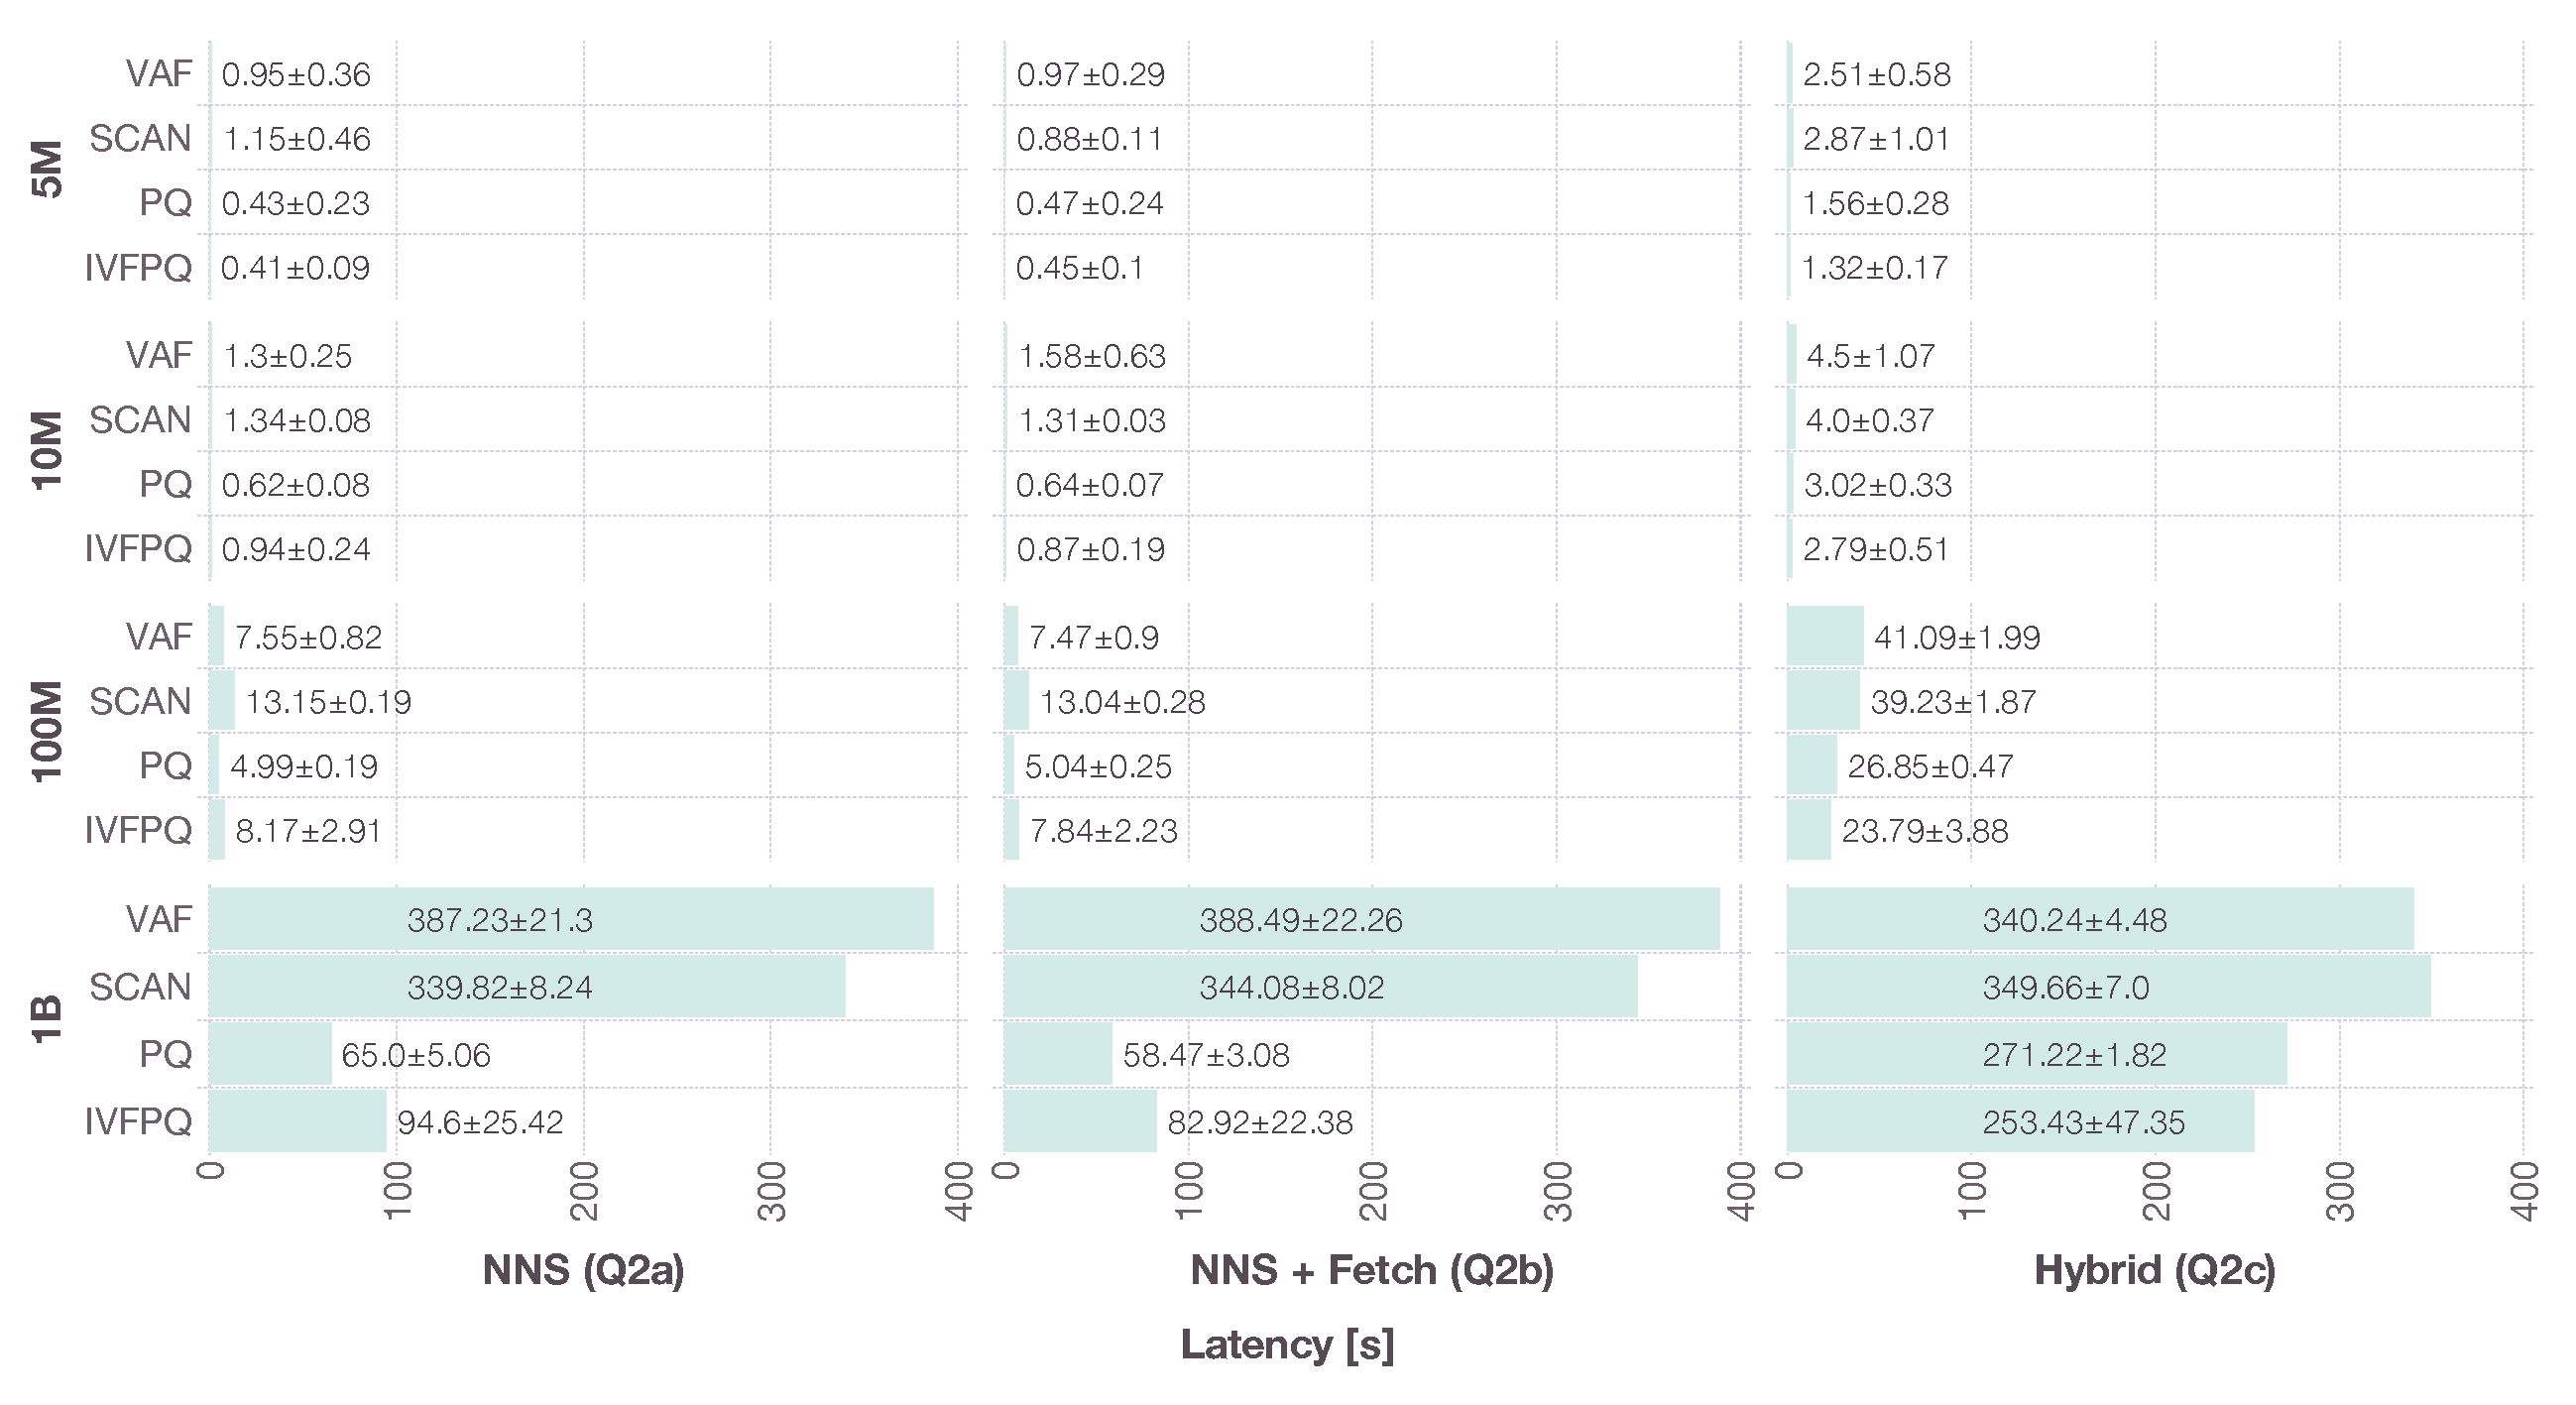
\includegraphics[width=1.55\textwidth]{figures/bignns/cottontail/bignns-cottontail-runtime}
        \caption {\cottontail{}'s latency in seconds for different workloads (x-axis) on different shards of the Deep 1B dataset using different execution strategies (y-axis).}
        \label{figure:cottontail_runtime}
    \end{figure}
\end{landscape}

In our first experiment, we executed the simple \acrshort{nns} workload (Q2a). The results are depicted in \Cref{figure:cottontail_runtime}. Brute-force search took between $0.95 \pm 0.36 \, \si{\second}$ (5 million) and $339.82 \pm 8.24 \, \si{\second}$ (1 billion). We can observe, that the \acrshort{vaf} index brings only minor advantages for the smaller datasets but reduces execution time by almost \SI{4}{\second} for the 100 million entries dataset. This is an artifact of the query execution engine, which uses less than the assigned 32 workers for the smaller collections because of the derived \acrshort{cpu} costs. Unfortunately, \acrshort{vaf} seems to perform poorly for the 1 billion entries dataset, where it is outperformed by an entity scan by more than \SI{40}{\second}. We believe this to be due to the many random accesses necessary for entries that could not be filtered out. If one considers a filter efficiency of approximately 90\% as advertised by \cite{Weber:1998Va}, one must still fetch $100$ million entries through random access, which seems more expensive than simply scanning the entire collection.

We can also clearly see, that using the \acrshort{pq} and IVF\acrshort{pq} index reduces execution time significantly, but at the cost of impaired quality, which is below $0.5$ on average for both recall and \acrshort{ndcg}, as can be seen in \Cref{figure:appendix_bignns_cottontail_nns_quality} (see \Cref{chapter:appendix_results}). Similarly to the analytics workload, we observe quite a large variance between individual queries. We expect, however, that the overall performance can be optimised by tuning the hyperparameters used upon index construction, specifically, the number of coarse and fine centroids. It is also worth noting, that the IVF\acrshort{pq} index does currently not support intra-query parallelism due to \cottontail{}'s partitioning model, i.e., the execution times we see for the IVFPQ index ($94.6 \pm 25.42 \, \si{\second}$ for $1$ billion entries) are always single-threaded. The execution plans are depicted in \Cref{figure:cottontail_nns_plan} and are fairly unsurprising: The use of \acrshort{vaf} and \acrshort{pq} constitutes a class 3 resp. class 1 index replacement according to Definitions \ref{definition:dfc_index_class_3} and \ref{definition:dfc_index_class_1}. The fetching of the \texttt{id} columns is pushed down to after the sort and limit operations, since this significantly reduces the amount of \acrshort{io} (only $1000$ fetches instead of scanning millions of entries).

\begin{figure}[p]
    \centering
    \begin{subfigure}[b]{\textwidth}
        \centering
        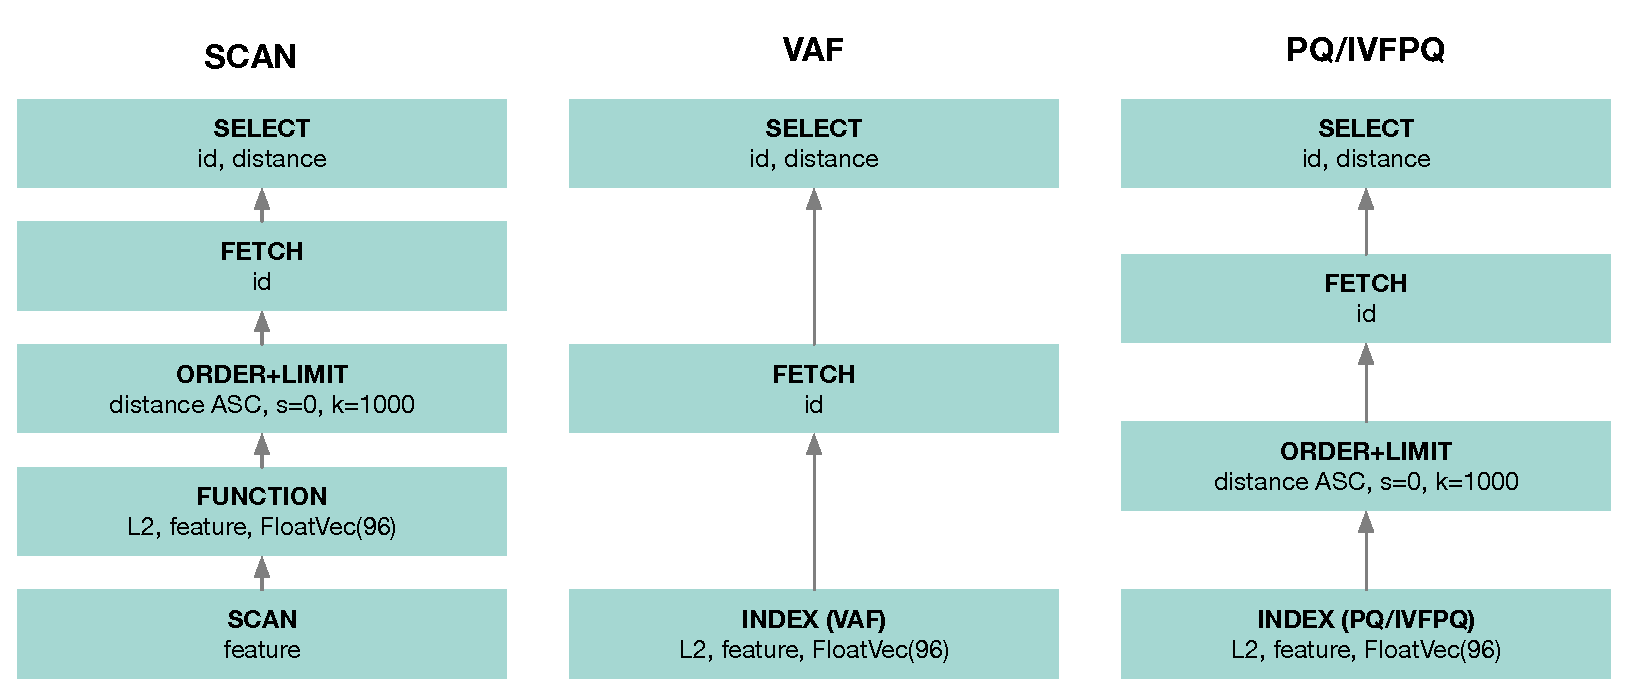
\includegraphics[width=\textwidth]{figures/bignns/cottontail/query-plan-nns}
        \caption{Simple \acrshort{nns}.}
        \label{figure:cottontail_nns_plan}
    \end{subfigure}
    \hfill
    \centering
    \begin{subfigure}[b]{\textwidth}
        \centering
        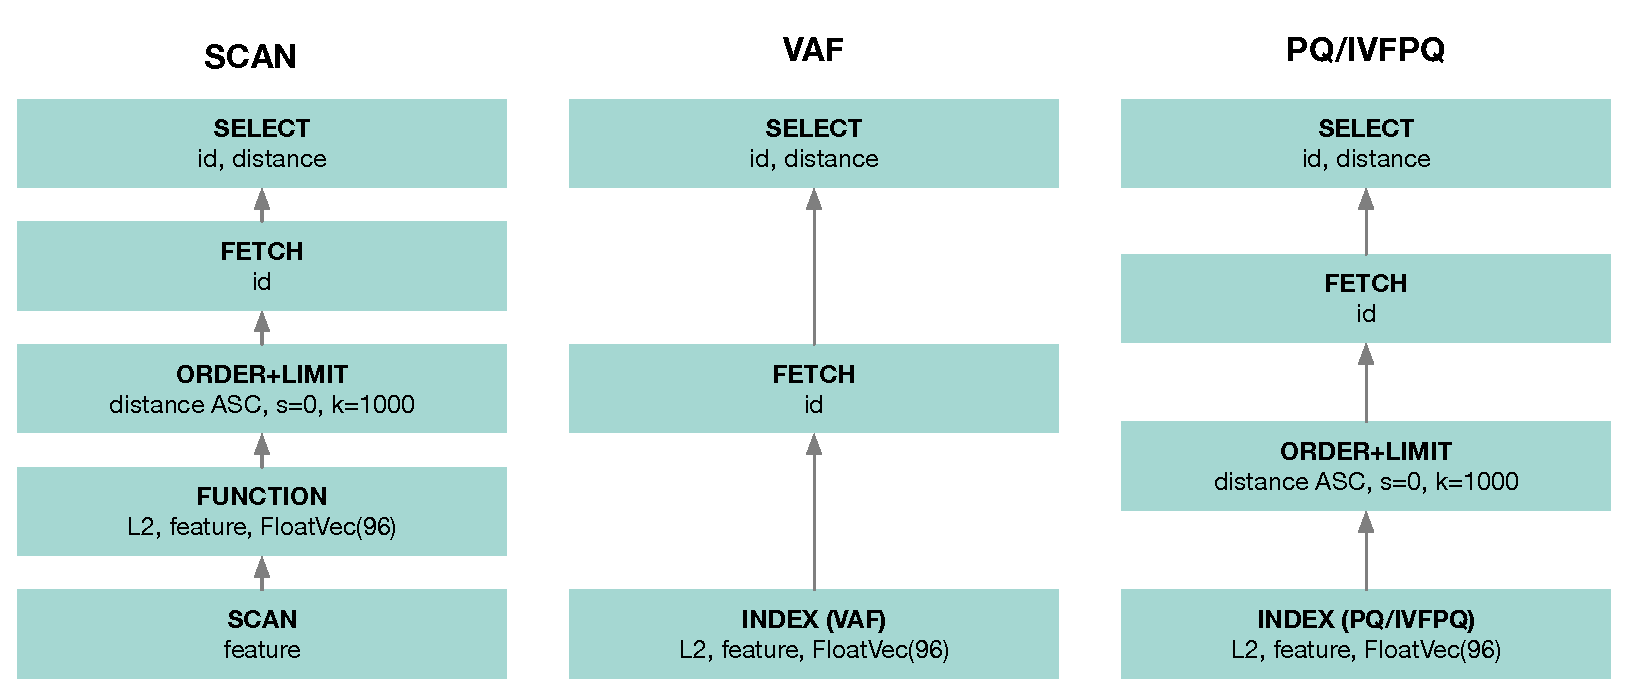
\includegraphics[width=\textwidth]{figures/bignns/cottontail/query-plan-nns}
        \caption{\acrshort{nns} and fetching of vectors.}
        \label{figure:cottontail_nns_fetch_plan}
    \end{subfigure}
    \hfill
    \centering
    \begin{subfigure}[b]{\textwidth}
        \centering
        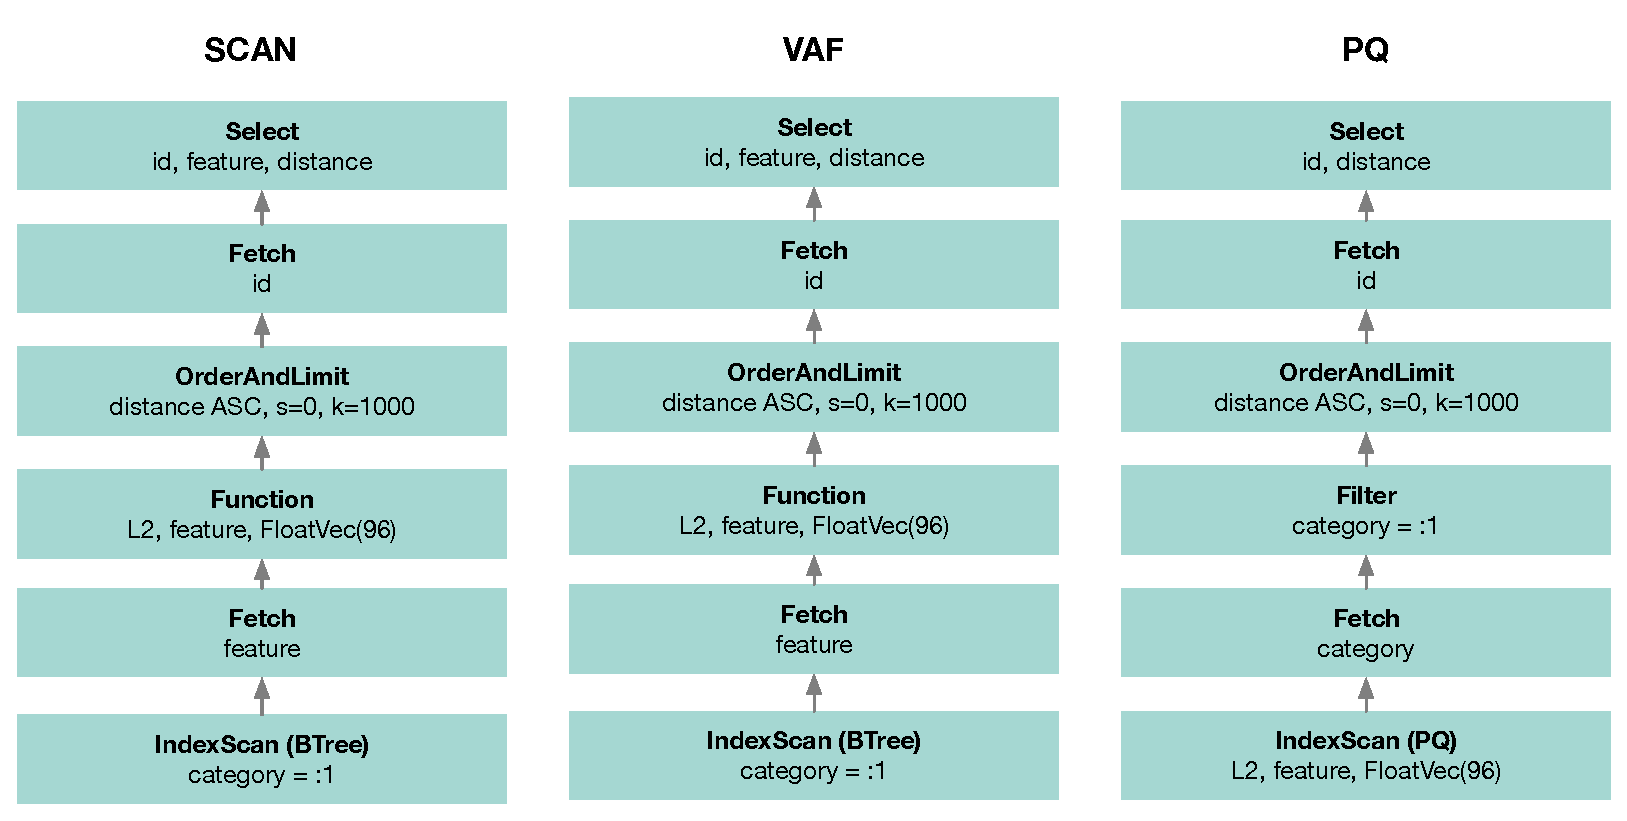
\includegraphics[width=\textwidth]{figures/bignns/cottontail/query-plan-hybrid}
        \caption{Hybrid query with Boolean filter.}
        \label{figure:cottontail_hybrid_plan}
    \end{subfigure}
    \caption{Execution plans produced by \cottontail{} for different query workloads prior to intra-query parallelisation. The use of the \acrshort{vaf} and \acrshort{pq} index was enforced using query hints.}
    \label{figure:cottontail_plans}
\end{figure}

Our second experiment involved the combined \acrshort{nns} and fetching of the resulting vectors. One can see in \Cref{figure:cottontail_nns_fetch_plan} that in terms of execution plan, accessing this additional column does not make a difference. Since both the plan involving the entity scan as well as the \acrshort{vaf} index scan produce the \texttt{feature} column early on, there is no need to fetch it later. Only for the \acrshort{pq} index -- which uses a distance approximation that is obtained without accessing the \texttt{feature} column -- an additional fetch is required. Consequently, the execution times are very similar to the simple \acrshort{nns} as one can see in \Cref{figure:cottontail_runtime} (NNS + Fetch). The numbers for a sequential scan range between $0.68 \pm 0.06 \, \si{\second}$ (5 million) and $344.08 \pm 8.02 \, \si{\second}$ (1 billion). The impact of the additional fetching of $1000$ feature columns is negligible for the \acrshort{pq} index, which can be attributed to the fact that the fetch is pushed until after the $s,k$-selection by the optimiser. We expect the impact of this fetching step to become more important for larger values of $k$ but it should remain negligible since typically, $k << N$. The quality metrics shown in the appendix (\Cref{figure:appendix_bignns_cottontail_nns_fetch_quality}), are comparable to those of the first experiment, exhibiting the same low numbers and high variance.

For the final experiment, we executed hybrid queries, i.e., \acrshort{nns} was restricted to a subset of the data that matches a Boolean predicate. The predicate involves a simple equality check that should effectively limit the exhaustive \acrshort{nns} to roughly $\frac{1}{10}$ of the collection. The values for a sequential scan range between $1.47 \pm 0.15 \, \si{\second}$ (5 million) and $349.66 \pm 7.0 \, \si{\second}$ (1 billion) with very similar numbers for the \acrshort{vaf} and \acrshort{pq} indexes. To make sense of these values, we again turn to the query plans illustrated in \Cref{figure:cottontail_runtime} (Hybrid). The sequential scan was executed with the help of a $B^{+}$-tree index, which speeds up the Boolean filtering. Unfortunately, the current implementation of the \acrshort{vaf} index cannot natively accommodate Boolean predicates, since it constitutes a class 3 index replacement according to \Cref{definition:dfc_index_class_3} and therefore, a special implementation of the index would be required\footnote{It is, however, unclear if such an implementation would be beneficial in practice.}. Consequently, a $B^{+}$-tree scan was executed instead. In contrast, the \acrshort{pq} index can be combined with Boolean predicates, since it constitutes a class 1 index replacement according to \Cref{definition:dfc_index_class_1}. However, one can see in \Cref{figure:cottontail_runtime} (NNS + Fetch) that the advantage of using the \acrshort{pq} index is negligible.
This can be attributed to the fact that a fetch operation for the \texttt{category} column must be executed for every entry before executing the filtering. The \acrshort{io} overhead is much larger than the speed-up gained through the \acrshort{pq} index. This is confirmed by the numbers we see for the IVF\acrshort{pq} index, which restricts the scan to a small subset of the collection. Similarly to the IVF\acrshort{pq} index, the $B^{+}$-tree index does currently not allow for parallel evaluation due to \cottontail{}'s partitioning model. This is severely limiting for the hybrid queries and something that should be addressed in the future. The \acrshort{ndcg} and recall values are again shown in \Cref{chapter:appendix_results} (\Cref{figure:appendix_bignns_cottontail_hybrid_quality}).

In summary, all modes of operation fail to deliver interactive latency for very large collections, which currently is the price that must be paid for being bound to disk. It is to be noted, however, that \cottontail{} does not employ any caching other than a page cache. We presume that such advanced caching of, e.g., signatures could result in a considerable speed-up.

\subsection{Milvus}
For executing queries in Milvus, the mode of operation is slightly different than it is for \cottontail, since Milvus requires a data collection to be available in main memory, to be able to query it. Therefore, every query consists of two steps: Loading the collection and then executing the query once the collection is ready. We have obtained the elapsed time for loading and query execution separately, so that we can consider the individual components. The way queries can be specified is outlined in \Cref{listing:milvus_query}. We show the Python instead of the Java syntax, because it is less verbose and more readable, assuming, that the functionality of the two client libraries is identical.  

\begin{lstlisting}[language=Python, caption={Example of a similarity search query in a collection ``images'' using a two-dimensional query vector and the Euclidean distance. Before executing the query, the data collection must be loaded.}, label=listing:milvus_query, numbers=none]
    from pymilvus import Collection
    
    # Load an existing collection.
    collection = Collection("images")      
    collection.load()

    # Perform search.
    query = [[0.0, 0.0]]
    params = {"metric_type": "L2", "params": {"nprobe": 10}}
    results = collection.search(
        data=query, anns_field="feature", param=params, limit=10
    )
\end{lstlisting}

Across all workloads, we compared the performance of two different types of indexes: The \texttt{FLAT} index is the equivalent of a sequential scan and it is the only index in Milvus that guarantees a recall of $1.0$. The \texttt{IVF\_SQ8} index uses an inverted file of clusters and limits the search to a subset of these clusters based on the parameters provided by the user and an initial distance calculation between the query and the cluster centres. This approach is comparable to cluster pruning \cite{Chierichetti:2007Finding} or the two-stage quantisation process described in \cite{Jegou:2010Product}, where each vector is mapped to an inverted list using a coarse quantiser. In addition to limiting the search space, the \texttt{IVF\_SQ8} index also compresses the \SI{4}{\byte} (\texttt{float}) into a \SI{1}{\byte} (\texttt{int8}) presentation, which significantly reduces memory and \acrshort{cpu} usage by up to 70\%. We built the \texttt{IVF\_SQ8} index beforehand using $4096$ clusters and instructed Milvus to consider $1024$ and $2048$ (query parameter \texttt{nprobe}) clusters respectively, when searching the collection.

\begin{landscape}
    \begin{figure}[p]
        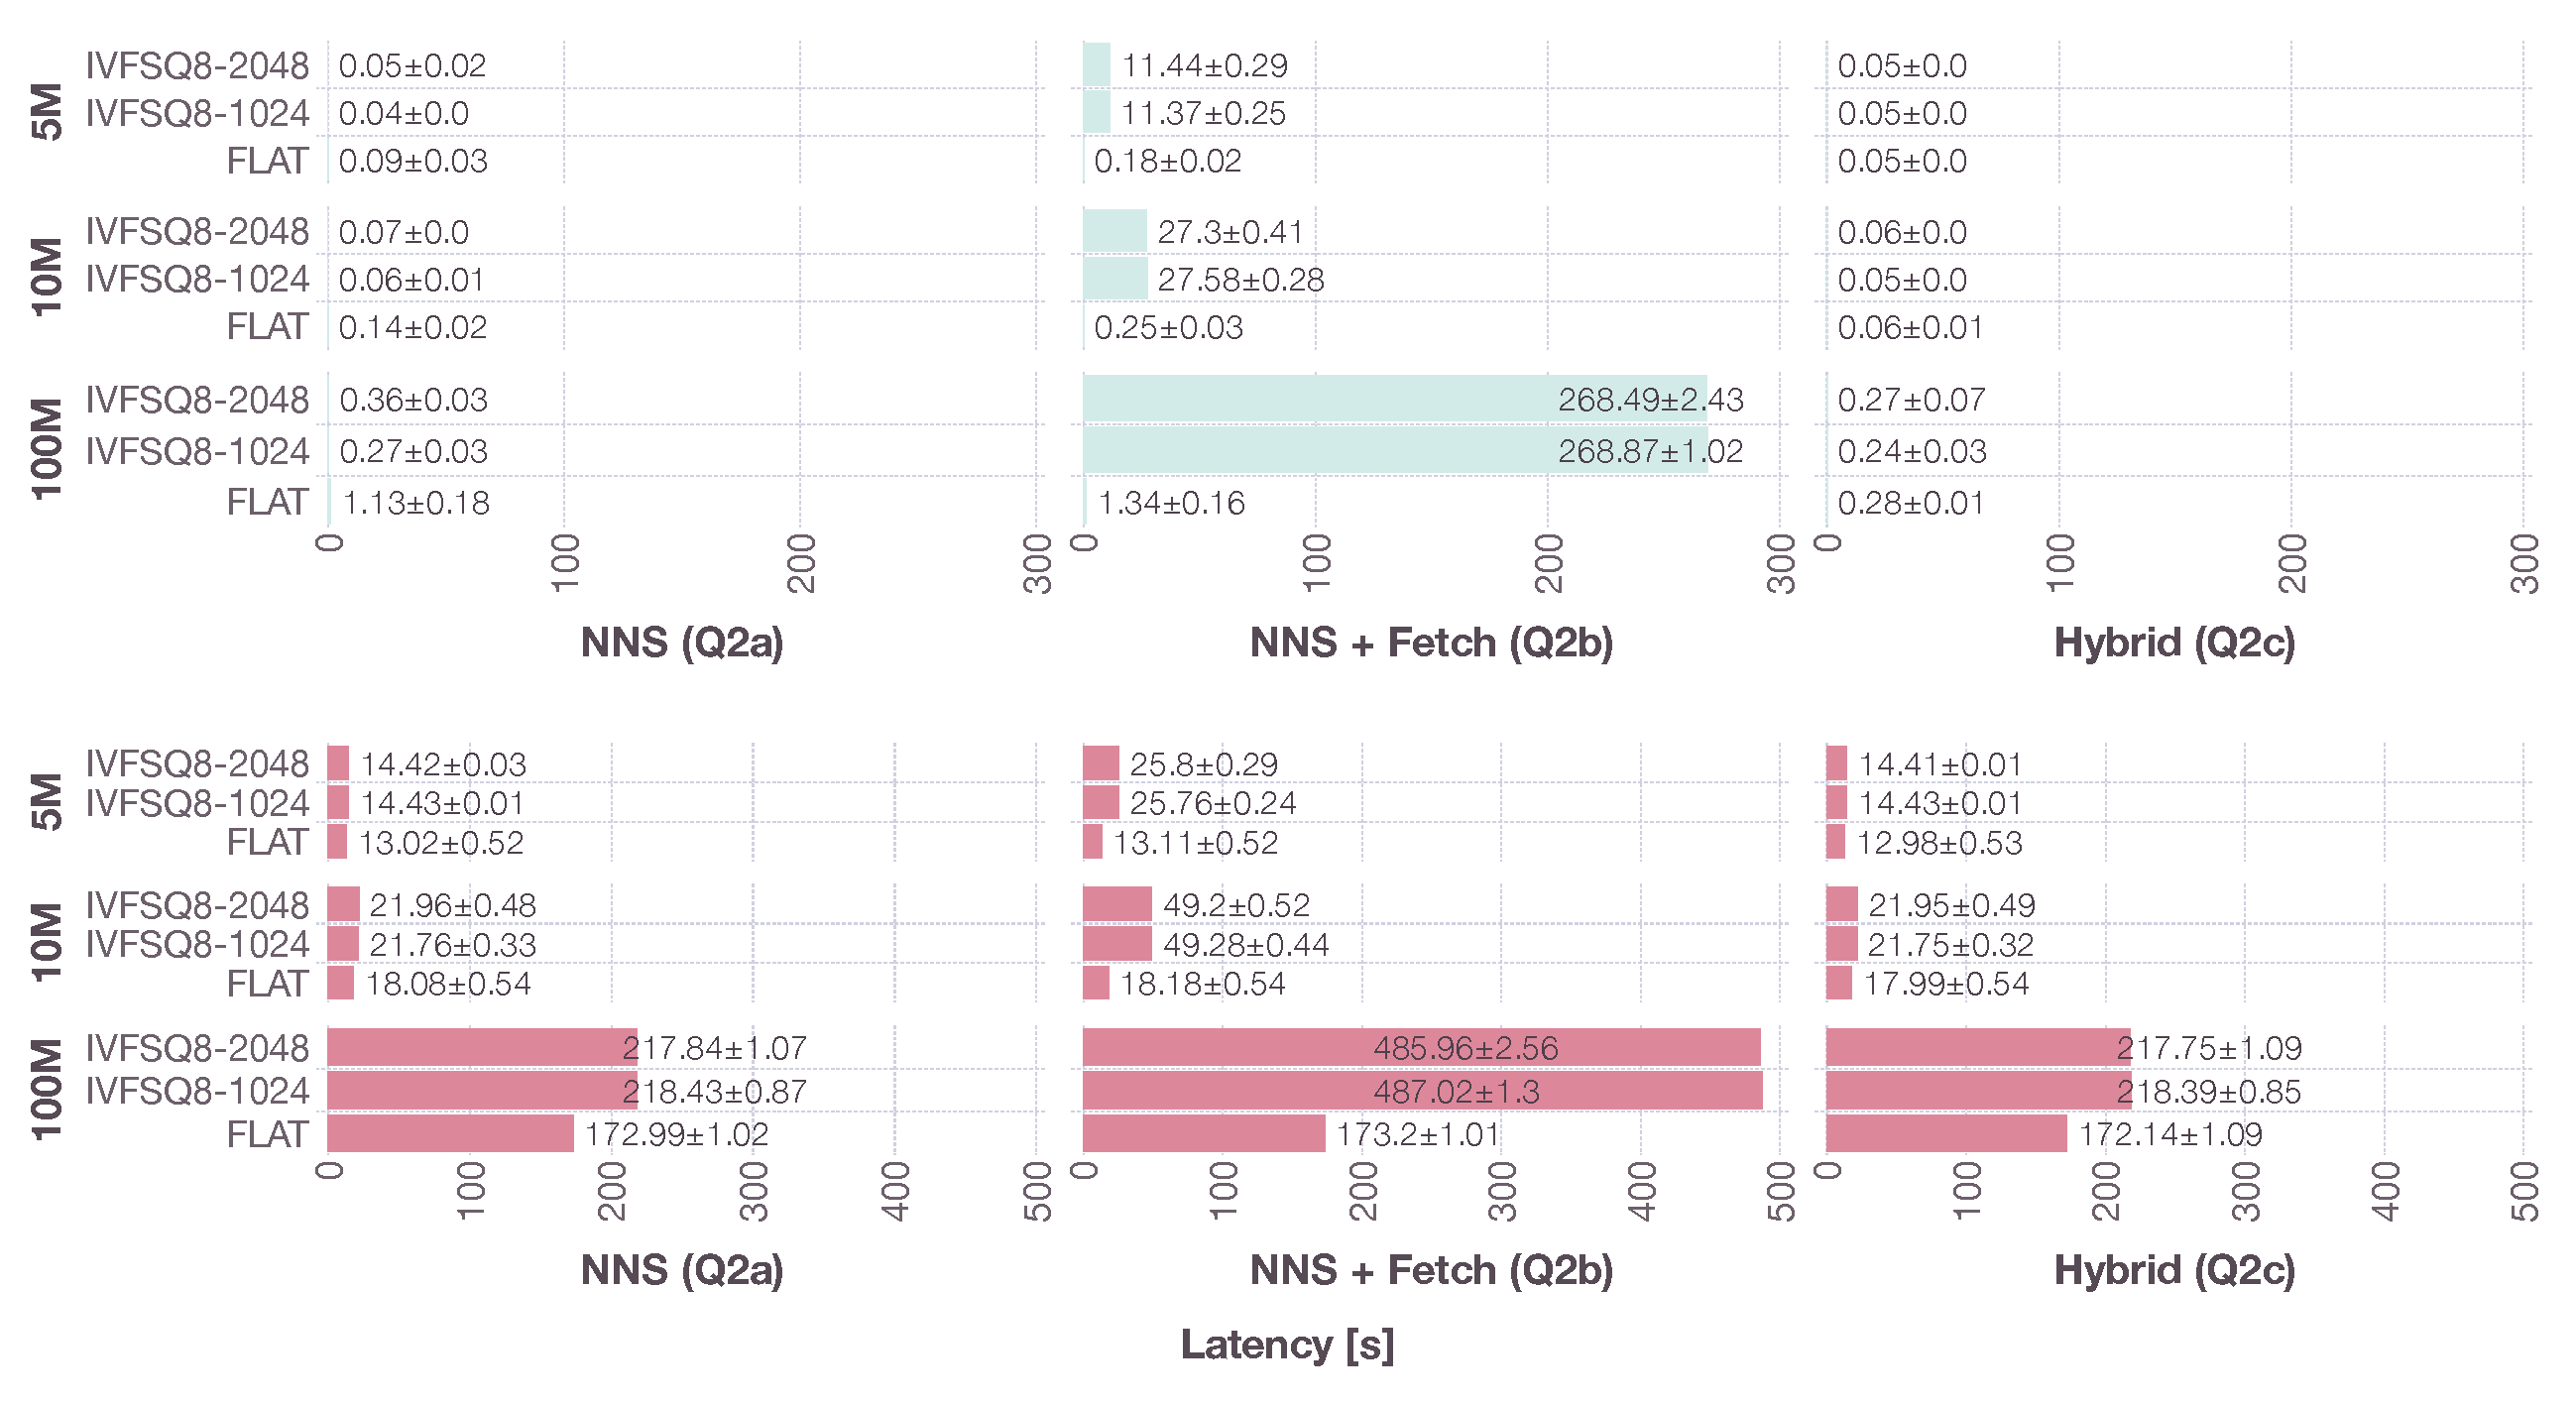
\includegraphics[width=1.6\textwidth]{figures/bignns/milvus/bignns-milvus}
        \caption{Milvus's latency in seconds for different workloads (x-axis) on different shards of the Deep 1B dataset using different access methods (y-axis), with (red) and without (mint) time used for loading the data from disk.}
        \label{figure:milvus_runtime}
    \end{figure}
\end{landscape}

In our first experiment we executed the simple \acrshort{nns} workload (Q2a). The results are depicted in \Cref{figure:milvus_runtime}. We can summarise that even for brute-force search (\texttt{FLAT}), query execution speed is very impressive once a collection has been loaded into main memory. For our test collection, it took between $0.09 \pm 0.03 \, \si{\second}$ (5 million) and $1.3 \pm 0.18 \, \si{\second}$ (100 million) to execute a query, all the while retaining a perfect recall and \acrshort{dcg} of $1.0$. However, if one considers time required to load a collection from disk to be part of the query time, these numbers rise to between $13.02 \pm 0.52 \, \si{\second}$ and $172.99 \pm 1.02 \, \si{\second}$. If one loads a collection once to then execute many queries thereafter, the performance provided by Milvus is very desirable as the cost of loading the collection can be amortised over time. However, if a large number of collections must be queried without the ability to predict which one, and not all collections can be pre-loaded, query execution time is expected to deteriorate. Furthermore, the requirement to load the collection prior to querying it turned out to be an insurmountable roadblock for the shard that contained 1 billion entries. Milvus was unable to load the collection as it ran out of available memory. We can confirm that Milvus indeed used up the entire \SI{376}{\giga\byte} of free \acrshort{ram} on the node.

In an attempt to alleviate the memory pressure, we also considered the \texttt{IVF\_SQ8} index, which seems a logical choice due to its data compression characteristics. Unfortunately, using this index instead did not resolve the problem of collection loading, since, Milvus always loads the indexes and the original data. Nevertheless, there are two interesting insights from the measurements:
\begin{enumerate*}[label=(\roman*)]
    \item \texttt{IVF\_SQ8} brings considerable speed-up for raw query execution time, especially for larger collections (roughly \SI{1}{\second} faster on 100 million shard),
    \item however, it exacerbates the performance impact of collection loading, since the indexes must be loaded in addition to the raw data.
\end{enumerate*}

The second experiment involved the combined \acrshort{nns} and fetching of the resulting vectors. Unfortunately, Milvus currently does not support the returning of vectors in an \acrshort{nns}, which is why this is a two-step process. First, the \acrshort{nns} is executed to subsequently look up the vectors for the resulting primary keys in a second query. We measure the time for both steps. The results are depicted in \Cref{figure:milvus_runtime} (Q2b). The additional fetching step, while cumbersome, does not seem to have a negative impact in cases where the \texttt{FLAT} index is used. However, use of the \texttt{IVF\_SQ8} index seems to lead to a significant deterioration of the query performance for the fetching step, adding between \SI{10}{\second} (5 million) and more than \SI{250}{\second} (100 million) to the total query execution time. We do not have an explanation for this and consider it to be abnormal behaviour.

Last but not least, we did execute hybrid queries, wherein \acrshort{nns} was restricted to a subset of the data that was filtered by a simple predicate. In Milvus, this is a query primitive that is part of the similarity search \acrshort{api}. The results are visualised in \Cref{figure:milvus_runtime} (Q2c) and do not hold any surprises. In-memory query execution speed is again outstanding whereas the time required to load a collection is significant. Interestingly, the \texttt{IVF\_SQ8} did not seem to have a negative impact on query execution speed, which confirms our suspicion that the deterioration observed in the second experiment must be considered a bug. 

We refrain from visualising \acrshort{ndcg} and recall values but can report that both always remained at $1.0$ for \texttt{FLAT} and around $0.99$ for all queries that used the \texttt{IVF\_SQ8} index.

\subsubsection{Qualitative Assessment}
While very convincing in terms of sheer execution speed, the current version of Milvus also has limitations that we list here for future reference:

\begin{itemize}
    \item Milvus currently only supports the Euclidean and Inner Product distance for single-precision floating point embeddings. There is no way to use other metrics or data types.
    \item Milvus does not support proximity-based search strategies other than \acrshort{nns}. However, according to the official GitHub issue tracker, \footnote{See https://github.com/milvus-io/milvus/issues/17599/; accessed August 2022.} range search is due for the 2.2.0 release. 
    \item Milvus cannot retrieve the feature vectors as part of an \acrshort{nns} query, i.e., they must be fetched in an additional lookup step based on the primary key. This issue is also due to be addressed in the 2.2.0 release. \footnote{See https://github.com/milvus-io/milvus/issues/16538/; accessed August 2022.}
    \item Milvus can only maintain a single index per feature column. This effectively limits the set of available distance functions to one, since most indexes must be trained for a specific distance.
\end{itemize}

In addition, we have observed that as Milvus uses up all the memory during collection loading, it behaves erraticlly making it difficult to unload the collection again. In some of our runs, Milvus started to reload the same collection after being restarted after a crash, effectively rendering the entire instance unusable for several hours.

\section{High-Dimensional Index Maintenance}
\label{section:hd_index_maintenance_evaluation}

With this evaluation, we demonstrate \cottontail{}'s ability to process incremental changes to data collections that hold a high-dimensional index structure. It is a test of the index maintenance mechanism described in \Cref{section:hd_index_maintenance} and of the transaction support \cottontail{} provides. The setup of this experiment is slightly different than that of all previous ones, in that it involves different workloads that run concurrently. The evaluation starts by creating an entity and loading it with $1$ million entries. We again use the Yandex Deep 1B ($d = 96$) dataset as a basis here and we start with the first one million vectors, i.e., the state of the collection at the beginning is identical for all runs. After data loading has completed, we generate and build an index -- either a \acrshort{vaf} ($35$ marks per vector component) or a \acrshort{pq} index ($8$ subspaces, $1024$ centroids) -- and start the actual measurement once it is ready. We run three threads simultaneously: 

The first thread runs a loop that performs a batch insert operation per cycle. For a single insert, we randomly draw between $100$ and $5000$ entries from the Yandex Deep 1B dataset. The range can be calibrated by a user-defined factor $c_{\texttt{ins}} \in [0.0, 1.0]$. The second thread runs a loop that randomly deletes between $100$ and $5000$ entries per cycle based on their ID. We use the sequential nature of the ID and a blacklist to make sure that every ID is only selected once to prevent deletes that have no effect. Again, the range can be calibrated by a user-defined factor $c_{\texttt{del}} \in [0.0, 1.0]$. Both the insert and the delete takes place in a dedicated transaction. Between cycles there is a pause of \SI{50}{\milli\second} to \SI{500}{\milli\second} to simulate operations that arrive randomly.

The third thread continuously executes \acrshort{nns} queries using the query vectors from the Yandex Deep 1B ground truth dataset. One \acrshort{nns} query explicitly uses the previously created index whereas the other query employs a brute-force scan to obtain the ground truth. As in previous experiments, we use query hints to nudge \cottontail{} in either direction. Furthermore, we prohibit intra-query parallelism to reduce noise. To make sure that the two queries operate on the same state of the database, they are executed in a single transaction \footnote{If we were to execute the queries without an explicit transaction, we would expect differences between the two results due to interleaving changes.}. We also obtain the query plan to verify that the index is used. 

In our first experiment, we run the workload for \SI{30}{\minute} using different factors, $c_{\texttt{ins}}$ and $c_{\texttt{del}}$, to steer the ratio of inserts and deletes. While it runs, we gauge how the collection, the speed-up, i.e., the difference in latency between brute-force and indexed search for \acrshort{nns}, and the quality of the results develop.

\begin{figure}[p]
    \centering
    \begin{subfigure}[b]{\textwidth}
        \centering
        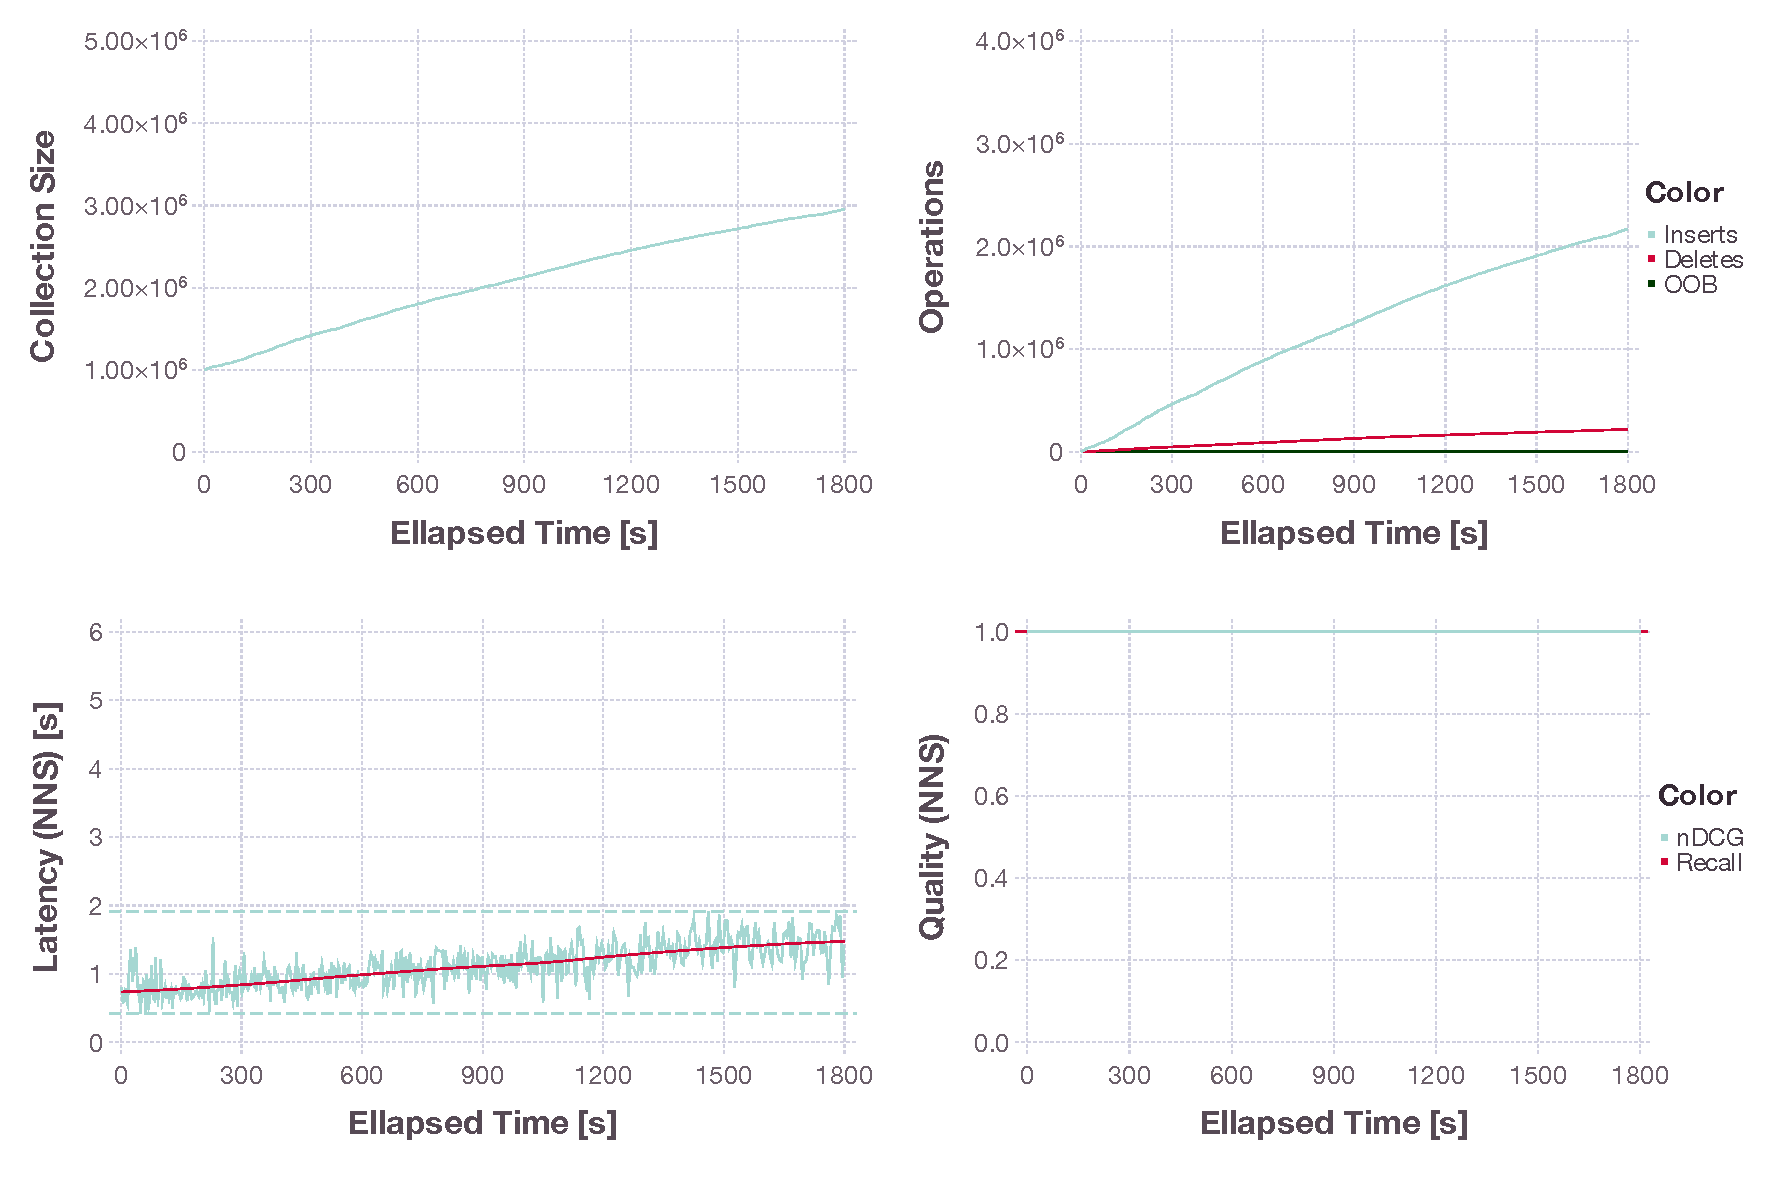
\includegraphics[width=\textwidth]{figures/index/index-vaf-adaptiveness-90-10-no-rebuild}
        \caption{Index adaptiveness measurements for \acrshort{vaf} index; for $c_{\texttt{ins}} = 0.9$ , $c_{\texttt{del}} = 0.1$.}
        \label{figure:index_adaptiveness_vaf_90_10}
    \end{subfigure}
    \hfill
    \centering
    \begin{subfigure}[b]{\textwidth}
        \centering
        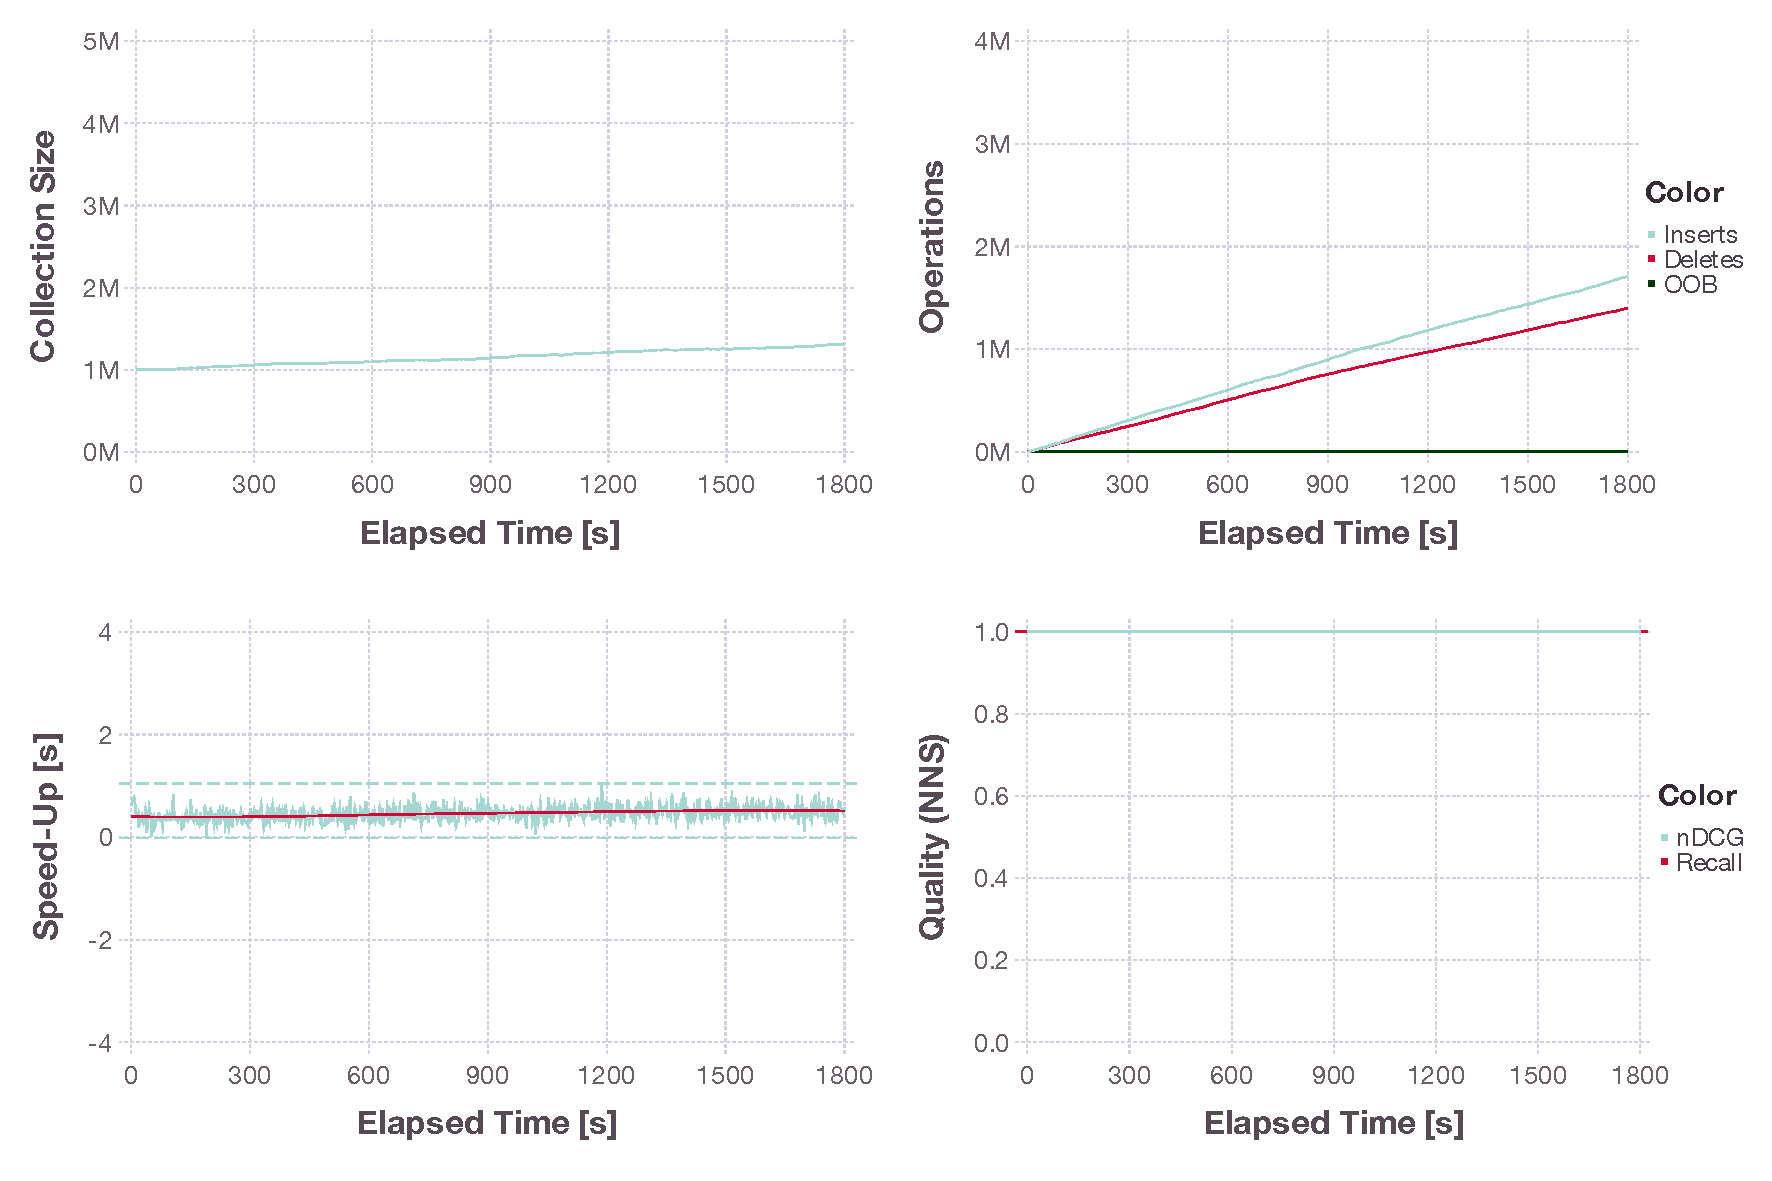
\includegraphics[width=\textwidth]{figures/index/index-vaf-adaptiveness-50-50-no-rebuild}
        \caption{Index adaptiveness measurements for \acrshort{vaf} index; for $c_{\texttt{ins}} = 0.5$ , $c_{\texttt{del}} = 0.5$.}
        \label{figure:index_adaptiveness_vaf_50_50}
    \end{subfigure}
    \caption{Index adaptiveness measurements for \acrshort{vaf} index for two different values of $c_{\texttt{ins}}$ and $c_{\texttt{del}}$, showing the size of the collection (top left), the number of accumulated insert and delete operations (top right), speed-up for \acrshort{nns} using the index (bottom left), and quality of the \acrshort{nns} query with respect to ground truth (bottom right) over time (x-axis).}
    \label{figure:index_adaptiveness_vaf}
\end{figure}

\begin{figure}[p]
    \centering
    \begin{subfigure}[b]{\textwidth}
        \centering
        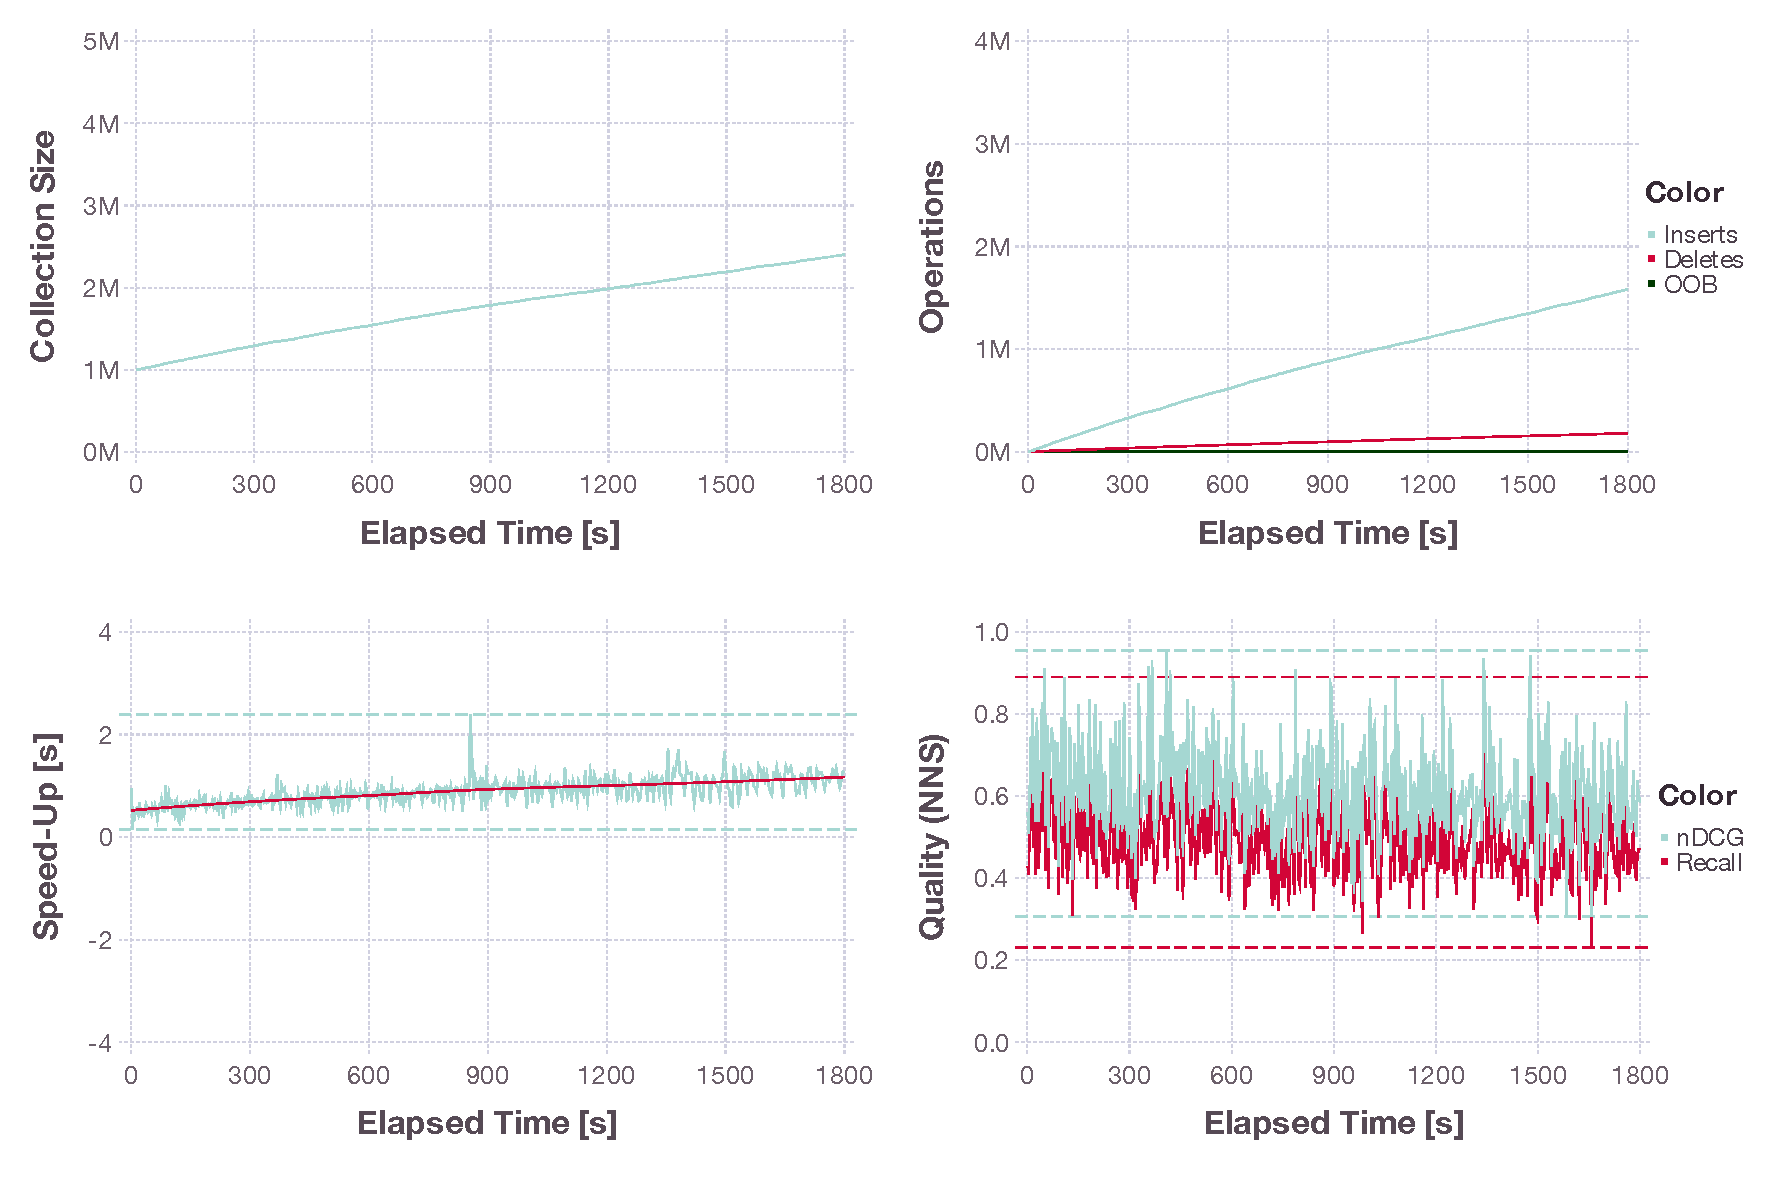
\includegraphics[width=\textwidth]{figures/index/index-pq-adaptiveness-90-10-no-rebuild}
        \caption{Index adaptiveness measurements for \acrshort{pq} index; for $c_{\texttt{ins}} = 0.9$, $c_{\texttt{del}} = 0.1$.}
        \label{figure:index_adaptiveness_pq_90_10}
    \end{subfigure}
    \hfill
    \centering
    \begin{subfigure}[b]{\textwidth}
        \centering
        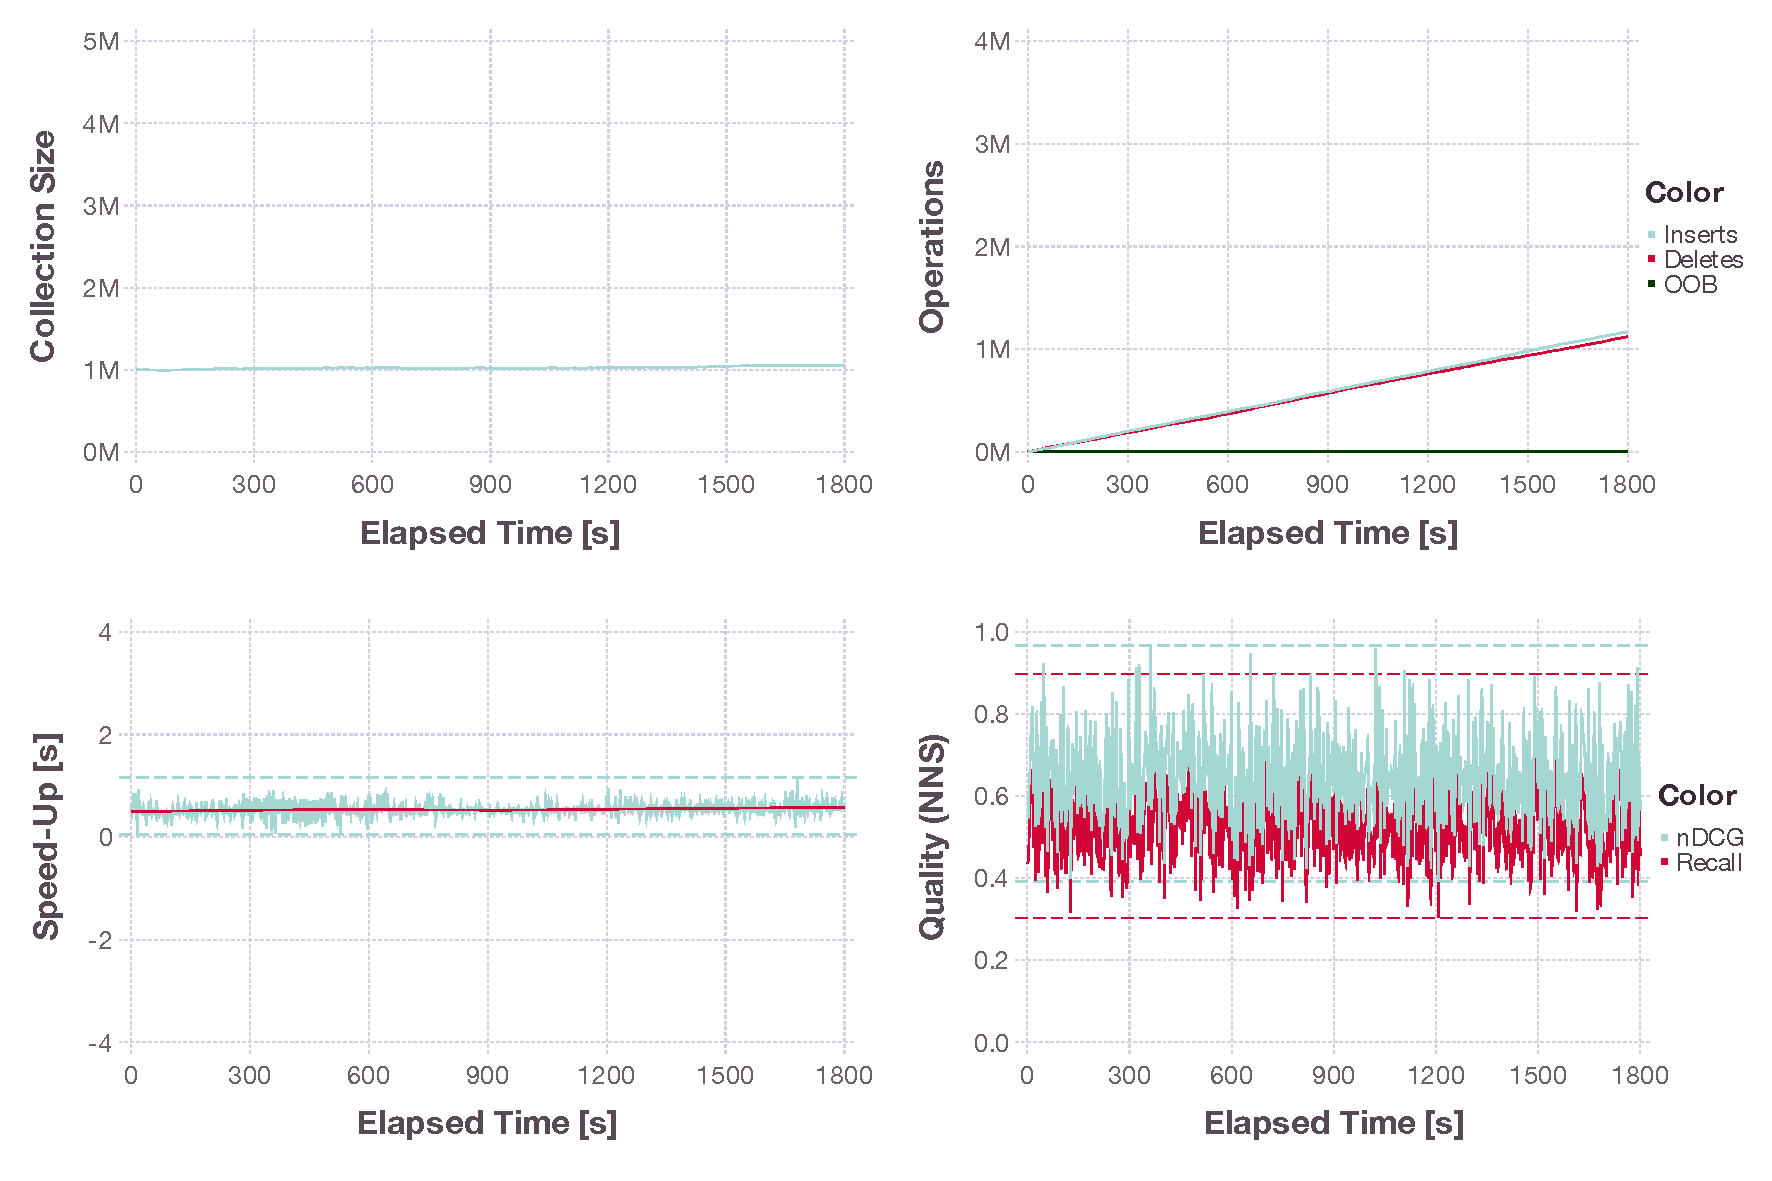
\includegraphics[width=\textwidth]{figures/index/index-pq-adaptiveness-50-50-no-rebuild}
        \caption{Index adaptiveness measurements for \acrshort{pq} index; for $c_{\texttt{ins}} = 0.5$, $c_{\texttt{del}} = 0.5$.}
        \label{figure:index_adaptiveness_pq_50_50}
    \end{subfigure}
    \caption{Index adaptiveness measurements for \acrshort{pq} index for two different values of $c_{\texttt{ins}}$ and $c_{\texttt{del}}$, showing the size of the collection (top left), number of accumulated insert and delete operations (top right), speed-up for \acrshort{nns} using the index (bottom left), and quality of \acrshort{nns} with respect to the ground truth (bottom right) over time (x-axis).}
    \label{figure:index_adaptiveness_pq}
\end{figure}

The plots for the first experiment are depicted in \Cref{figure:index_adaptiveness_vaf} (VAF) and \Cref{figure:index_adaptiveness_pq} (PQ) and we can make several observations: For the workload with $c_{\texttt{ins}} = 0.5$ and $c_{\texttt{del}} = 0.5$ we see that the collection size remains more or less constant and with it both speed-up and quality delivered by the \acrshort{vaf} (\Cref{figure:index_adaptiveness_vaf_50_50}) as well as the \acrshort{pq} (\Cref{figure:index_adaptiveness_pq_50_50}) index.

In contrast, speed-up for executing \acrshort{nns} shows a slight upward trend for both the \acrshort{vaf} (\Cref{figure:index_adaptiveness_vaf_90_10}) and \acrshort{pq} (\Cref{figure:index_adaptiveness_pq_90_10}) for $c_{\texttt{ins}} = 0.9$ and $c_{\texttt{del}} = 0.1$. This is to be expected, since the indexes are designed to scale better with the linear increase of collection size. We cannot observe any visible deterioration in terms of speed-up building up over time. Similarly, both recall and \acrshort{ndcg} remain steady for both indexes over the course of the measurement despite the concurrent write operations, which is the desired and thus expected behaviour. On an unrelated note, we can also see how unpredictable and noisy the quality of the results produced by the \acrshort{pq} index is, which assumes values of between $0.9$ and $0.2$. It is also to be noted that growth of the collection is slower for \acrshort{pq} despite being governed by the same benchmark logic. We suspect this to be a consequence of the higher overhead incurred by generating the \acrshort{pq} signature upon insert. This also explains why there is a slight net-growth for \acrshort{vaf} $c_{\texttt{ins}} = 0.5$ and $c_{\texttt{del}} = 0.5$ workload, as we generally expect deletes to be slower than inserts, which indeed seems to be the case for \acrshort{vaf} (but not for \acrshort{pq}).

We have argued in \Cref{section:hd_index_maintenance}, that we expect the performance of an index to depend on how well the data fits the (unknown) distribution of the corpus the index was built upon. To get an indication of this, we have also recorded the component-wise minimum and maximum at the start of the run (i.e., of the first $1$ million entries). Every time a new vector is inserted, we check if a component exceeds that minimum and maximum and record such entries as out-of-bounds (OOB). For this first experiment, wherein we use the collection in its unaltered state, we can spot no discernible growth in these entries and indeed the data suggest that only a few $100$ appear among the first $2$ million inserts. This is an indication albeit not a proof of the validity of our assumption.

To test our method with data that does not exhibit this kind of well-behavedness, we run a second experiment in which we introduce noise. This \emph{jitter} is simply a random number of configurable magnitude $M$ that is added to each vector component prior to insert. We run this experiment for \SI{90}{\minute} and randomly apply the same transformation to 50\% of the query vectors, i.e., some queries exhibit the same noise while others do not. After \SI{30}{\minute} we trigger an asynchronous rebuild of the index structure to observe its effect.

\begin{figure}[p]
    \begin{subfigure}[b]{\textwidth}
        \centering
        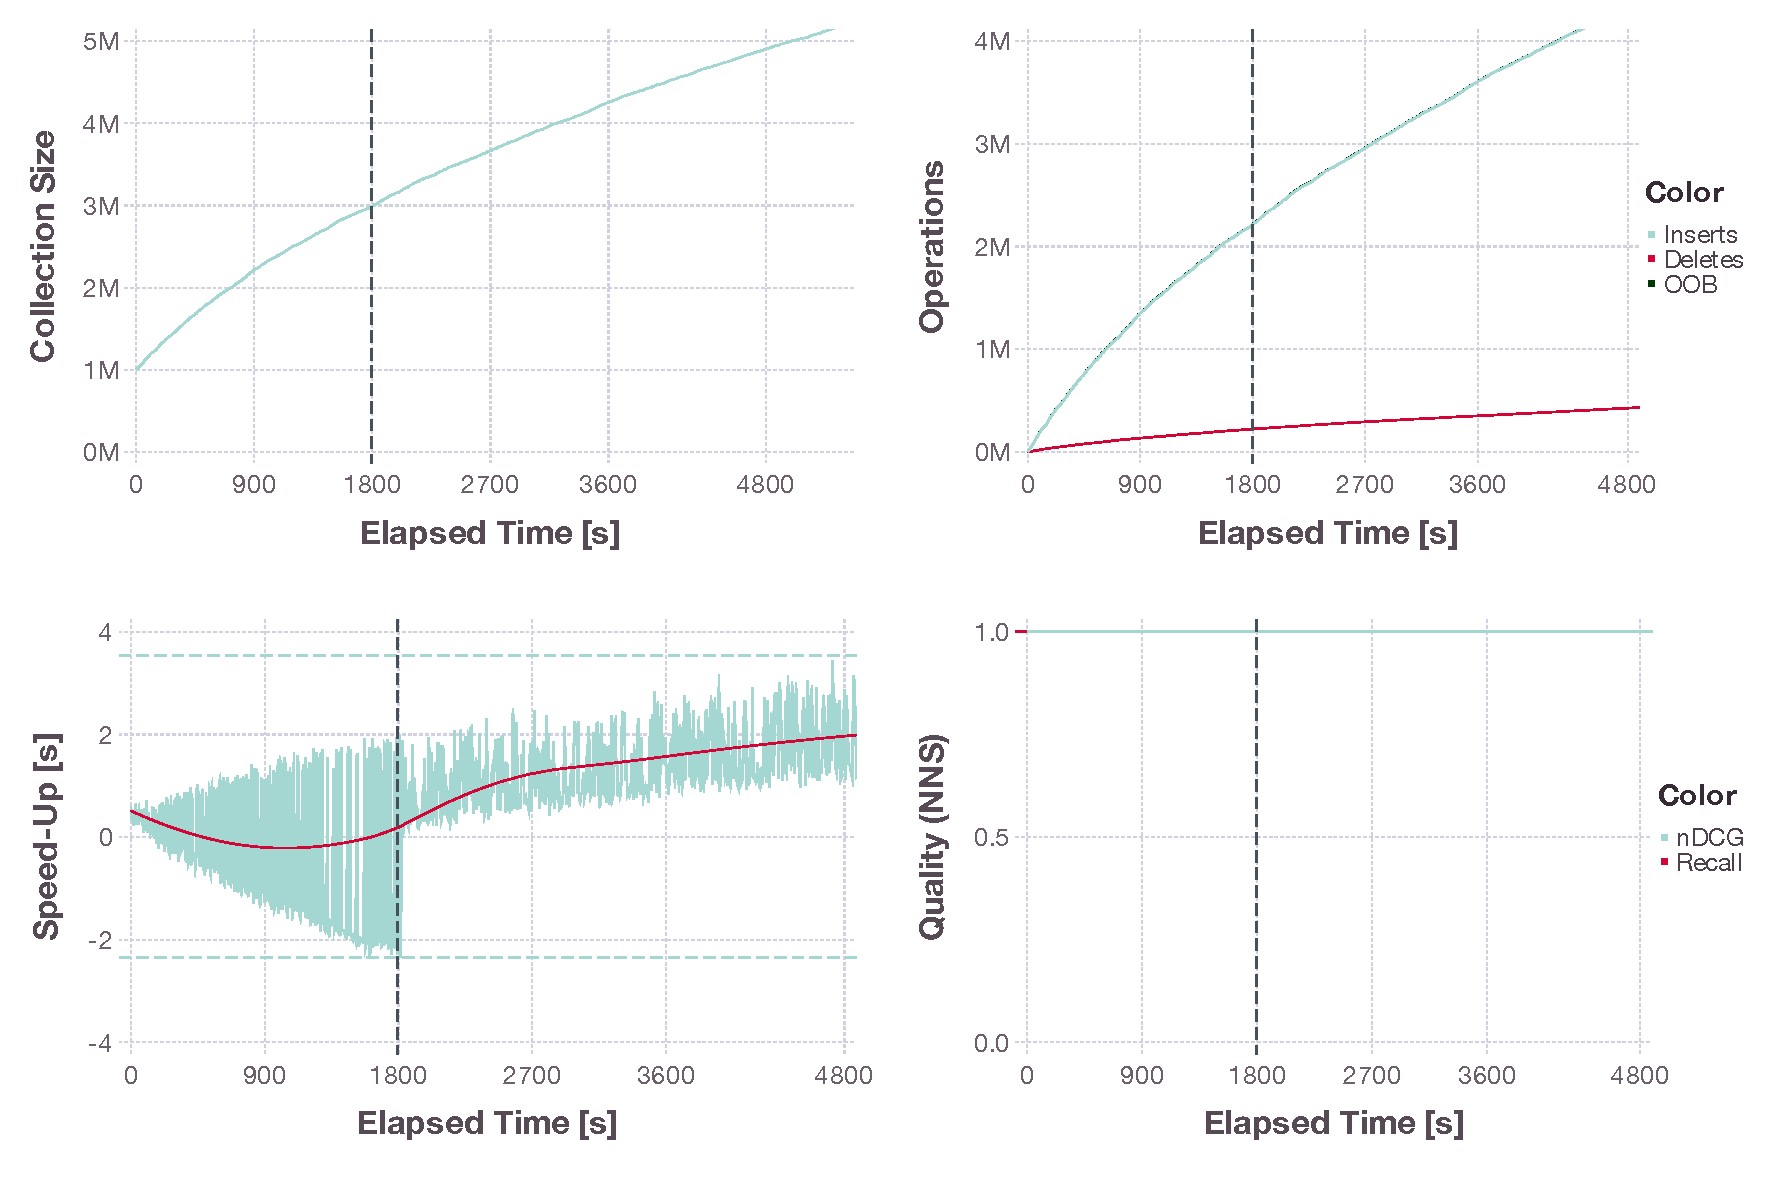
\includegraphics[width=\textwidth]{figures/index/index-vaf-adaptiveness-90-10-with-rebuild-and-jitter}
        \caption{Index adaptiveness measurements for \acrshort{vaf} index; for for $c_{\texttt{ins}} = 0.9$ , $c_{\texttt{del}} = 0.1$, $M = 100$.}
        \label{figure:index_adaptiveness_vaf_90_10_jitter}
    \end{subfigure}
    \hfill
    \centering
    \begin{subfigure}[b]{\textwidth}
        \centering
        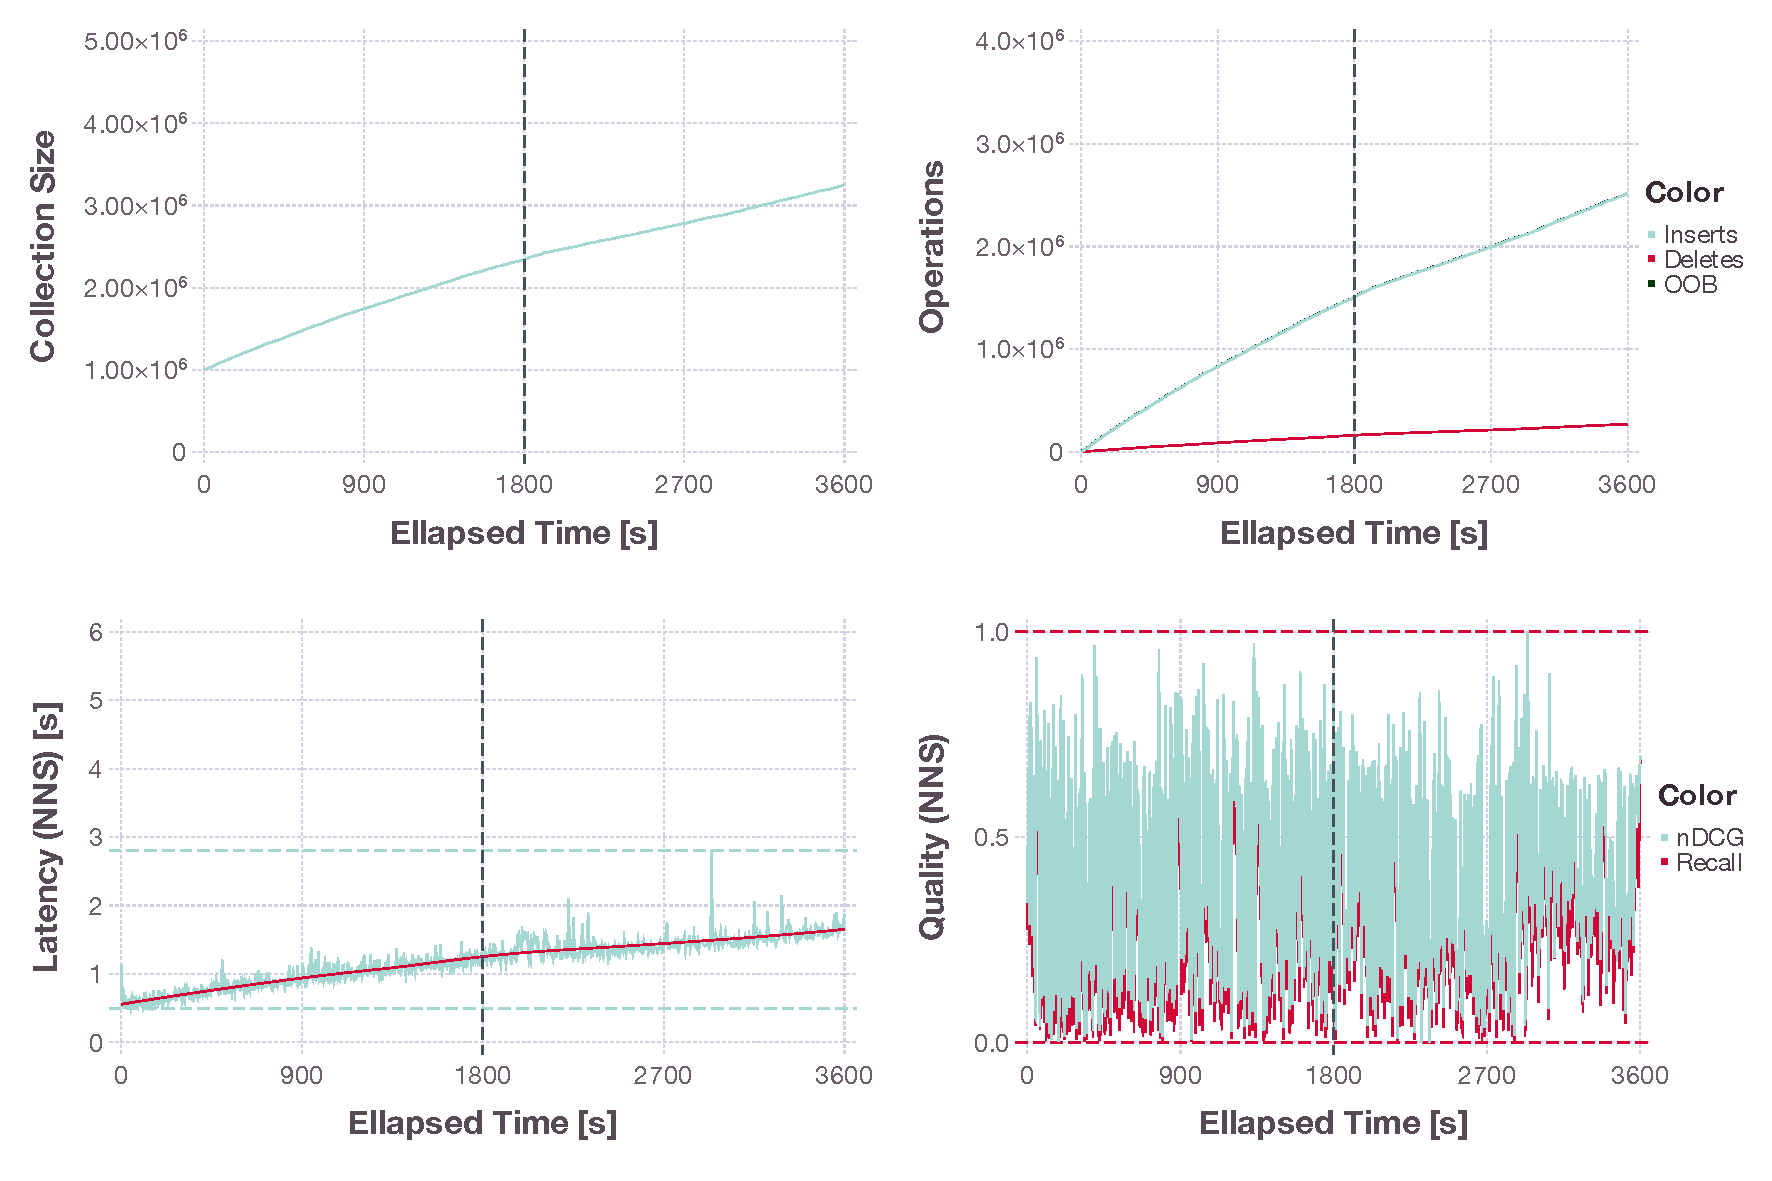
\includegraphics[width=\textwidth]{figures/index/index-pq-adaptiveness-90-10-with-rebuild-and-jitter}
        \caption{Index adaptiveness measurements for \acrshort{pq} index; for for $c_{\texttt{ins}} = 0.9$ , $c_{\texttt{del}} = 0.1$, $M = 100$.}
        \label{figure:index_adaptiveness_pq_90_10_jitter}
    \end{subfigure} 
    \caption{Index adaptiveness measurements for the \acrshort{vaf} and \acrshort{pq} index, showing the size of the collection (top left), the number of accumulated insert and delete operations (top right), speed-up for \acrshort{nns} using the index (bottom left), and quality of the \acrshort{nns} query with respect to the ground truth (bottom right) over time (x-axis). Data and queries exhibit a random noise and index rebuild is started after \SI{30}{\minute} (grey, dashed line).}
    \label{figure:index_adaptiveness_jitter}  
\end{figure}

The plots for the second experiment are depicted in \Cref{figure:index_adaptiveness_jitter} and we break them down for the two indexes: For \acrshort{vaf} (\Cref{figure:index_adaptiveness_vaf_90_10_jitter}), we see constant quality of $1.0$ over the entire measurement -- both for \acrshort{ndcg} and recall. This is expected since \acrshort{vaf} should retain quality guarantees even for very noisy data. However, speed-up provided by the index deteriorates significantly during the first \SI{30}{\minute} to the point where it is actually slower than the linear scan. Furthermore, we observe a massive increase in variance between individual queries. This can be attributed to the random noise that is added to some query vectors. Queries that do not exhibit that noise are still filtered out by the index quite effectively (between 85\% and 95\% efficiency). In contrast, the filtering capacity continuously drops for noisy queries as noisy data accumulates. This can be explained by how the \acrshort{vaf} works. Since the index still reflects the original distribution without noise, vectors that match this distribution can be distinguished with a constant resolution and will be assigned to one of the $m^d$ cells ($m$ denoting the number of marks per dimension) leads to \SI{4.81e16}{} possibilities. All the noisy vectors accumulate on the edge of the high-dimensional lattice, of which there are only $2 * m * d$ (which leads to \SI{7720}{} possibilities). As soon as a noisy vector is being queried, it is very likely to end up in one of the $2 * m * d$ cells which, in turn, is likely to be occupied by a large number of vectors, all of which must be fetched from disk to perform a distance calculation. This is why this effect increases as the benchmark proceeds. After \SI{30}{\minute}, we trigger the asynchronous re-indexing and it finishes shortly thereafter. The effect becomes visible immediately, as speed-up and especially the variance decrease significantly. The index rebuild itself has a slight effect on the concurrent \acrshort{dml} operations, which take more time but can continue normally.

For the \acrshort{pq} index, the deterioration manifests itself in the quality, which now oscillates between $0.9$ and $0.0$. The explanation is similar to the one for the \acrshort{vaf}: The old index is still capable of assigning query vectors that do not exhibit any noise to their proper centroid and can therefore reliably approximate the distance for them. Noisy vectors get assigned to some centroid but the distortion in distance becomes too big for reliable \acrshort{nns}. After \SI{30}{\minute}, we also trigger the asynchronous re-indexing. In the case of \acrshort{pq}, the overhead incurred is clearly visible in the throughput for both insert and delete, which otherwise continue normally. After about \SI{52}{\minute}, we see a normalisation in the quality metric in that the variance is less severe. However, quality is still far from optimal even after the rebuild has concluded, which can be attributed to the parametrisation of the index.

\newpage
 
\section{Summary, Related Work and Discussion}
\label{section:discussion}

With the evaluation we have demonstrated the applicability of the concepts introduced in \Cref{chapter:system_model} to practical scenarios using our reference implementation, \cottontail{}. Even though \cottontail{} was unable to compete with Milvus in terms of raw processing speed, we consider this evaluation to be a success. Maintaining and accessing all the relevant data on disk incurs an overhead that makes it difficult or even impossible to reach the processing speed of pure in-memory systems like Milvus. This was pointed out by L. Amsaleg, who stated: \emph{``When purposely dealing with secondary storage, it is hard if not impossible to beat high-dimensional indexing solutions that have been designed to run in main memory. This is unfortunately true even for collections that might fit in main memory, as enforcing durability etc. generates a substantial overhead''} \cite{Amsaleg:2014Database} (p. 12). Regardless of these limitations, \cottontail{} still seems to perform pretty well against Milvus, especially when the time required for loading data from disk is considered as well. In our experiments, during the time that Milvus required to load a collection, \cottontail{} could query that same collection between $15$ (VAF) to $34$ (PQ) times, all the while retaining the flexibility to switch between collections and/or execute different types of workloads that Milvus could not (e.g., range search). Our experiments have also demonstrated the limitations of pure in-memory processing in cases where collections simply do not fit into main memory, regardless of how optimised the execution engine may be.

\subsection{Generalised Proximity-Based Queries}

The notion of generalised, proximity-based operations as an extension to the relation algebra described in \Cref{section:generalised_proximity_based_ops} provides us with the ability to construct and execute a wide range of query workloads in a much more flexible way than purpose-built systems such as Milvus \cite{Wang:2021Milvus} can provide. Furthermore, the proposed algebra enables the \acrshort{dbms} to decompose and optimise queries based on the needs expressed by a system user and the parameters of the system itself. 

In the past decades, many information retrieval models have been proposed \cite{Umano:1983Retrieval,Salton:1983Extended,Wong:1985Generalized}. Some of these models are set-based \cite{Salton:1983Extended,Umano:1983Retrieval}, and thus similar to the relational model \cite{Codd:1970Relational}, while others are based entirely on the vector space model that considers documents to be high-dimensional vectors \cite{Wong:1985Generalized}. Our approach uses the relational model as a foundation and integrates the notion of complex data types (e.g., vectors), functions that operate on these types, as well as scoring and ranking as explicit extensions in way that enables its use beyond mere multimedia retrieval. In that it follows an established tradition of extending the expressive power of \acrshort{sql} and the relational model \cite{Libkin:2003Expressive}, which has been practiced for many years \cite{Chengkai:2005RankSQL,Zhang:2006Boolean,Belohlavek:2007Relational}, as we have argued in \Cref{section:rel_extensions}. Conceptually, we see the proposed extensions as a first, minimally invasive step towards the realisation of the \emph{Extended Boolean Retrieval Model} as proposed in \cite{Salton:1983Extended}. In such a model, distances and scores can be employed to perform advanced operations such as fuzzy-set operations or similarity joins \cite{Umano:1983Retrieval,Zadeh:1996Fuzzy,Bohm:2001Fast}. From our perspective and with an eye on analytics workloads, we would also like to see query primitives such a clustering or \acrshort{rnns} \cite{Korn:2000Influence} in that list of supported operations.

The convergence of information retrieval and databases as well as the addition of multimedia support have been a recurring subject at many of the database self-assessment meetings since the 1980s \cite{Agrawal:2008Claremont}. Unsurprisingly, many attempts at convergence have been made over the years at a conceptual \cite{Marcus:1996Foundations,Adjeroh:1997Multimedia,Watanabe:1998Multimedia}, logical \cite{Zhang:2006Boolean,Belohlavek:2007Relational}, and physical \cite{Silva:2010SimDB,Giangreco:2014Adam,Whang:2015DB,Giangreco:2016Adam,Yang:2020Pase} level. We follow that trend and, the model we propose provides a sound, theoretical foundation rooted in relational algebra and has been demonstrated to be useful in practical scenarios. 

An important, mental step that enables such simple, yet expressive models is that of ``separation of concerns'', or what \cite{Giangreco:2018Database,Ferro:2014Bridging} refer to as ``pragmatics'', which is in fact realised throughout the \vitrivr{} stack \cite{Rossetto:2016Vitrivr,Gasser:2019Multimodal}. While similarity search and retrieval may be the ultimate aim, from a database perspective, we merely execute simple primitives such as the evaluation of distance functions, sorting, and selection. By carefully ignoring the noise introduced by higher-level concepts such as documents, features, scores, and distances -- which may not be useful for data processing -- the database system can focus on its core purpose which is that of providing reliable and fast data management and access and leave the interpretation and advanced data modelling to upper-tier systems. This is a common approach in database research, and with our model we further move in such a direction, similar to computational databases such as SciDB \cite{Stonebraker:2013SciDB}, MonetDB \cite{Idreos:2012MonetDB}, or HypeR \cite{Hubig:2017HyPerInsight}, which focus on providing support for efficient computation close to where the data resides, without too strictly limiting the concrete application. Such systems form an active research field \cite{Luo:2018Scalable,Blacher:2022Machine} and might hold interesting benefits for the multimedia community. They constitute a stark contrast to systems with very focused applications such as Milvus \cite{Wang:2021Milvus}, Vald\footnote{See https://github.com/vdaas/vald/; accessed August 2022.}, or Qdrant\footnote{See https://github.com/qdrant/qdrant/; accessed July 2022.}.

Since \adampro \cite{Giangreco:2016Adam} is \cottontail{}'s predecessor and one of the inspirations for the work presented in this Thesis, we would also like to highlight the differences between its query model and our own. As outlined in \Cref{section:vitrivr_adam_adampro}, \cite{Giangreco:2018Database} proposes a new similarity operator $\tau_{\delta(\cdot,\cdot),a,q}(\relation)$ that \emph{``performs a similarity query under a distance $\delta(\cdot,\cdot)$ applied on an attribute $a$ of relation $\relation$ and compared to a query vector $q$''} \cite{Giangreco:2018Database} (p. 138). It then uses this operator to derive more restricted versions that basically consider \acrshort{nns} and range search ($\epsilon$NN) to be dedicated query primitives. As we have argued in \Cref{section:generalised_proximity_based_ops}, this model is very restrictive in its assumptions and to some extent violates the aspect of pragmatics as proposed by both \cite{Ferro:2014Bridging} and \cite{Giangreco:2018Database}.

In contrast, our model considers the distance computation to be the result of an arbitrary function invocation. We restrict ourselves to certain distance functions in practice but in theory, any function could be employed. Furthermore, we use the extended projection to make the derived distance explicit and we argue, that making the attribute explicit is what allows downstream processing such as normalisation (from distance to score) or combination of multiple scores to express score fusion or variants thereof \cite{Bohm:2001Fast}. Ultimately, we consider it to be at the discretion of the user to decide whether and how calculated attributes should be used and included and it should be the task of the query optimiser to take these decisions into account when preparing an efficient execution plan.

Consequently, the relational algebra extensions we propose are rather limited and lie well within the capabilities most modern \acrshort{dbms} possess today. In line with \cite{Abadi:2014Beckman,Abadi:2020Seattle}, we identify the efficient execution of the functions and computations involved using the available means in terms of hard- and software (e.g., \acrshort{simd}, \acrshort{gpu}), as important, future research directions. In order to enable fast execution, functions must be enriched with metainformation that allows for optimisation at different stages of the query planning and execution process. In addition, we also believe the relationship between functions and indexing techniques to be a promising avenue to explore. 

Nevertheless, other systems, such as Milvus \cite{Wang:2021Milvus}, take a similar approach to \cite{Giangreco:2016Adam} as they add query primitives for the different types of workloads they accommodate -- leading to a growing number of disjoint APIs for different purposes. We do not consider this a sustainable approach, since it ignores future workloads that may combine existing primitives in a different way (e.g., aggregating on distance or \acrshort{fns}). Furthermore, generating specialised blackbox operators for different types of high-level primitives unnecessarily limits the potential for optimisation by the \acrshort{dbms} and increases the complexity of the systems. 

\subsection{Query Planning and Cost Model}  
In \Cref{section:cost_model} we have proposed a cost model that takes the expected quality of results into account, and we have discussed methods that can be used to estimate that quality for different, known query plans. Our reference implementation \cottontail{} uses a query planner that leverages the aforementioned cost model to determine the optimal execution path given a query and a cost policy specified by the user, as demonstrated in \Cref{section:cost_model_evaluation}.

To the best of our knowledge, both aspects -- the estimation of quality as well as its use in a cost model for query planning -- are rather uncommon in multimedia search systems today. Even though the quality versus execution time trade-off is an implicit consequence of approximate solutions to proximity-based search in general and \acrshort{nns} in particular, there is very little research that considers this issue systematically, with a few, notable exceptions: \cite{Weber:2000Trading,Blok2001:Predicting,Siguroardottir:2005Quality}. This is reflected by the fact, that most state-of-the-art approximate index structures fail to provide any strong quality guarantees \cite{Echihabi:2021High}. Here we see a huge corpus for future research: On the one hand, we see a need for index structures that provide explicit quality guarantees such as \cite{Lu:2020VHP}. On other the hand, we should continue to explore system-level mechanisms that continuously evaluate the efficiency and effectiveness by which results have been produced and adjust the cost model accordingly. Such an empirical approach to query planning has already been proposed by \cite{Giangreco:2018Database}, however, taking only execution time into account. This goes into the direction of adaptive query processing \cite{Deshpande:2007Adaptive} and the cost model we propose can be seen as a foundation for a continuous control loop between the query execution engine and the query planner.

\subsection{High-Dimensional Index Maintenance}

Maintaining a durable and consistent state and providing transactional guarantees for data structures required for executing queries -- including secondary index structures -- is a basic trait shared by most if not all traditional \acrshort{sql} and NoSQL systems. For some reason, however, durability and the notion of isolation and consistency in the face of dynamic data are aspects often overlooked for high-dimensional indexing \cite{Amsaleg:2014Database,Hojsgaard:2019Index}, especially in combination \cite{Amsaleg:2014Database}. In \Cref{section:hd_index_maintenance}, we have proposed a system-level mechanism for maintaining high-dimensional index structures on disk and for processing incremental changes to the data in a transactional manner. The viability of the proposed mechanism but also its limitations were demonstrated in \Cref{section:hd_index_maintenance_evaluation}, based on two examples.

Despite an already huge corpus of research that dates back to the 1970s \cite{Bentley:1975Multidimensional,Guttmann:1984RTrees,Beckmann:1990RTree,Indyk1998:Approximate,Weber:1998Va,Jegou:2010Product}, high-dimensional indexing for \acrshort{nns} is still a very active research topic today \cite{Shimomura:2021Survey,Kraska:2018Case}. Since different index structures provide different properties in terms of scalability, performance, and quality (guarantees) and can potentially be employed for different tasks, we regard this work as pivotal for further extending the indexing capabilities of a multimedia \acrshort{dbms} such as \cottontail{}. One could argue that having a single index may be sufficient, however, we believe that in light of a \acrshort{dbms}'s ability to plan queries and of the different properties these indexes bring, having a choice is better. Furthermore, multiple indexes could also be combined to improve the quality of results and the speed of execution \cite{Giangreco:2018Database}.

In light of ever-growing data collections, the topic of disk-based \acrshort{anns} has been getting more attention lately, with a few, early examples \cite{Lejsek:2011NVTree,Lejsek:2009NVTree,Gudmundsson:2010Large} and new, emerging techniques such as DiskANN \cite{Jayaram:2019DiskANN} or SPANN \cite{Chen:2021SPANN}, which both advertise a hybrid in-memory/on-disk processing model and report impressive numbers for both latency and recall. However, in contrast to \cite{Lejsek:2011NVTree,Lejsek:2009NVTree,Hojsgaard:2019Index}, both these state-of-the-art algorithms do not consider dynamic data and operate on the premise that the complete data collection can be (re-)indexed. This severely limits their usefulness. Nevertheless, such efforts lay important groundwork for disk-based multimedia index maintenance and must simply be extended in terms of their ability to process incremental changes.

In \cite{Lejsek:2011NVTree,Lejsek:2009NVTree}, the authors propose the NV-tree, which is a disk-resident, high-dimensional index structure that provides transactional support \cite{Lejsek:2018Transactional} and thus allows for inserts, updates, and deletes. The NV-tree would make a great extension to \cottontail{} and we expect it to fully fit into the proposed model for index maintenance in that it is an index structure that does not fail per-se and should not exhibit deterioration due to dynamic data (i.e., it can be considered a corner case, like the $B^{+}$-tree). Unfortunately, however, the index structure itself seems proprietary and the available literature does not provide us with enough information to come up with our own implementation.

The subject of online indexing (i.e., processing incremental changes) has also been addressed by a several authors, for indexes such as \acrshort{pq} \cite{Xu:2018Online}, \acrshort{lsh} \cite{Cakir:2015Adaptive}, (e)\acrshort{cp} \cite{Hojsgaard:2019Index} and some graph-based methods \cite{Zhao:2022Approximate}. While the proposed methods lack a notion of index state and transactionality, and (with the exception of \cite{Hojsgaard:2019Index}) do not consider indexes to be durable data structures, these are still very important contributions towards robust write-models for different types of indexing techniques. 

We have also discussed different vector database systems in \Cref{section:vector_databases}, which all face the issue of dynamic data. Milvus \cite{Wang:2021Milvus}, for example, handles inserts by marking them with timestamps and it allows for configurable consistency levels that differ in the timestamps of entries that are being considered. Hence, it uses a kind of \acrshort{mvcc}-based consistency and concurrency control model, similarly to \cottontail. In contrast, deletes are not propagated to the indexes and instead enabled by setting bit mask for deleted entries and filtering them on the fly at query time. This method is reminiscent of the ``tombstone markers'' used in Apache Cassandra, which are thought to be culprits for major performance hits. However, it is not fully clear how the method employed by Milvus scales as changes accumulate. Nevertheless, some concepts employed by Milvus may be very interesting, e.g., the (re-)indexing of chunks rather than the entire data collection at once. Vald  advertises an ``asynchronous auto indexing'' that uses ``distributed index graphs'' to avoid locking the entire graph during indexing. However, it is not clear what type of guarantees are provided by this mechanism other than preventing a system-wide halt, and generally it seems, that the method is very specific to the NGT index used \cite{Iwasaki2016:Pruned}. Unfortunately, for Qdrant, we could not find any information as to how dynamic data and concurrency are handled.

